% SYNONYMS
 
%examine, study, investigate, explore, consider, analyse, review, outline
%propose, suggest, advance, offer, present, submit, prefer, initiate, recommend,  posit
%develop 	expand, reinforce, extend, broaden, enhance, elaborate, amplify, refine, improve, polish, perfect
% create, generate, produce, design, fabricate, manufacture, build, construct, erect,
%  group-category,  gather, mass, cluster, aggregation, collection, network, crowd, collection
% represents- depict, portray, render, delineate, show, illustrate,  characterize, paint, draw, sketch, indicate, identifies, denotes, symbolise, signifies
%examine- inspect, survey, scrutinize, enquire into, study, investigate,explore, consider, appraise,research, analyse, review,

\documentclass[format=acmsmall, screen=true]{acmart}
%\documentclass[10pt,a4paper]{article}
\usepackage{booktabs}  
\usepackage{float,caption}
\usepackage{algorithm,algcompatible,amsfonts} 
\usepackage{subcaption,multirow} 
\usepackage{tabularx,enumerate,amsmath,graphicx}
\usepackage{pifont,pbox}
\newcommand{\yeah}{\checkmark}
\newcommand{\nope}{ {\small \ding{55}} }

 %\email{etot5316@uni.sydney.edu.au}
%

\begin{document}



\setcopyright{acmcopyright}
\acmJournal{CSUR}
\acmYear{2018} \acmVolume{1} \acmNumber{1} \acmArticle{1} \acmMonth{1}
 \acmPrice{\$15.00}
 \acmDOI{10.1145/3203246}


\begin{CCSXML}
<ccs2012>
<concept>
<concept_id>10002944.10011122.10002945</concept_id>
<concept_desc>General and reference~Surveys and overviews</concept_desc>
<concept_significance>500</concept_significance>
</concept>
<concept>
<concept_id>10010147.10010257.10010258.10010260.10010229</concept_id>
<concept_desc>Computing methodologies~Anomaly detection</concept_desc>
<concept_significance>500</concept_significance>
</concept>
<concept>
<concept_id>10002950.10003648.10003688.10003693</concept_id>
<concept_desc>Mathematics of computing~Time series analysis</concept_desc>
<concept_significance>300</concept_significance>
</concept>
</ccs2012>
\end{CCSXML}

\ccsdesc[500]{General and reference~Surveys and overviews}
\ccsdesc[500]{Computing methodologies~Anomaly detection}
\ccsdesc[300]{Mathematics of computing~Time series analysis}

\author{Edward Toth}
\affiliation{%
    \institution{School of Information Technologies, The University of Sydney}
       \email{etot5316@uni.sydney.edu.au}
%   \city{ Sydney}
    \country{Australia}
}
%
\author{Sanjay Chawla }
\affiliation{%
    \institution{Qatar Computing Research Institute, Hamad bin Khalifa University }
    \email{schawla@qf.org.qa}
    \city{Doha}
    \country{Qatar}
}
 

%\input{Abstract}

%\begin{abstract}
%Given a portfolio of stocks, a series of frames in a surveillance video or even a group of people, how do we detect dynamic anomalous changes in their collective behaviors in an online fashion? 
% As a solution to this problem, we propose GRACE, an effective algorithm that is rapid and flexible in detecting significant changes in different aspects of group distributions.  
% 
%In this paper, we validate the theoretical distribution of test statistics computed in GRACE as well as demonstrate the effectiveness of GRACE as compared with state-of-the-art models. We also implement our proposed method on two real world applications; video footage recording the movement of pedestrians and a portfolio of health care stocks over a a twenty year period.  
%\end{abstract}

%Anomaly detection and change detection is an important research area with a vast range of domain applications. %Additional issues arise when involving group structures.  

\begin{abstract}
Pointwise anomaly detection and change detection focus on the study of individual data instances however an emerging area of research involves groups or collections of observations. From applications of high energy particle physics to healthcare  collusion,  group deviation detection techniques result in novel research discoveries, mitigation of risks,  prevention of  malicious collaborative activities and other interesting explanatory  insights.  In particular, static group anomaly detection   is the process of identifying groups that are not consistent with regular group patterns while dynamic group change detection  assesses significant differences in the state of a group  over a period of time. Since both group anomaly detection   and group change detection   share fundamental ideas, this survey paper provides a clearer and deeper understanding of group deviation detection  research in static and dynamic situations.  %by explains the underlying structure and key descriptive components for state-of-the-art techniques. 
\end{abstract} 
 \keywords{Group deviation detection, group anomaly detection, group change detection, machine learning, generative models, discriminative methods, hypothesis testing} 
 
 \title{  Group Deviation Detection Methods: A Survey }
\maketitle


\chapter{Deep Learning for Anomaly Detection: A Survey}
% \chapter{Introduction}
\label{chpt:survey}
\section{Introduction}

A common need when analyzing real-world data-sets is determining which instances stand out as being dissimilar to all others. Such instances are known as \emph{anomalies}, and the goal of \emph{anomaly detection} (also known as \emph{outlier detection}) is to determine all such instances in a data-driven fashion~\cite{chandola2007outlier}. Anomalies can be caused by errors in the data but sometimes are indicative of a new, previously unknown, underlying process; in fact Hawkins~\cite{hawkins} defines an outlier as an observation that {\it deviates so significantly from other observations as to arouse suspicion that it was generated by a different mechanism.} In the broader field of machine learning, the recent years have witnessed proliferation of deep neural networks, with unprecedented results across various application domains. Deep learning is subset of machine learning that achieves good performance and flexibility by learning to represent the data as nested hierarchy of concepts within layers of neural network. Deep learning outperforms the traditional machine learning as the scale of data increases as illustrated in Figure~\ref{fig:performanceCompare}. In recent years, deep learning-based anomaly detection algorithms has become increasingly popular and has been applied for diverse set of tasks as illustrated in Figure~\ref{fig:applications}; studies have shown that deep learning completely surpasses traditional methods~\cite{javaid2016deep,peng2015multi}. The aim of this survey is two fold, firstly we present a structured and comprehensive review of research methods in deep anomaly detection (DAD). Furthermore, we also discuss the adoption of  DAD methods across various application domains and assess their effectiveness.

% in both research and applications ~\cite{javaid2016deep}.

%performance comparision
\begin{figure}[h]
\centering
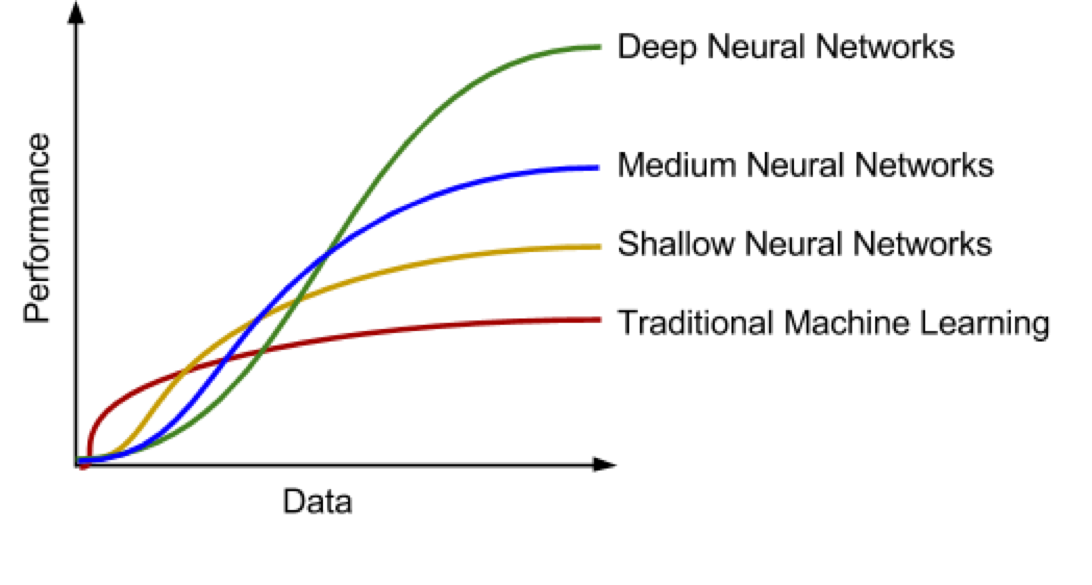
\includegraphics[scale=0.5]{images/traditionalVsDeepLearning}
\captionsetup{justification=centering}
\caption{Performance Comparison of Deep learning-based algorithms Vs Traditional Algorithms~\cite{deeplearningVstraditionalAlgorithms}.}
\label{fig:performanceCompare}
\end{figure}


%%Applications of deep learning based anomaly detection
\begin{figure}[h]
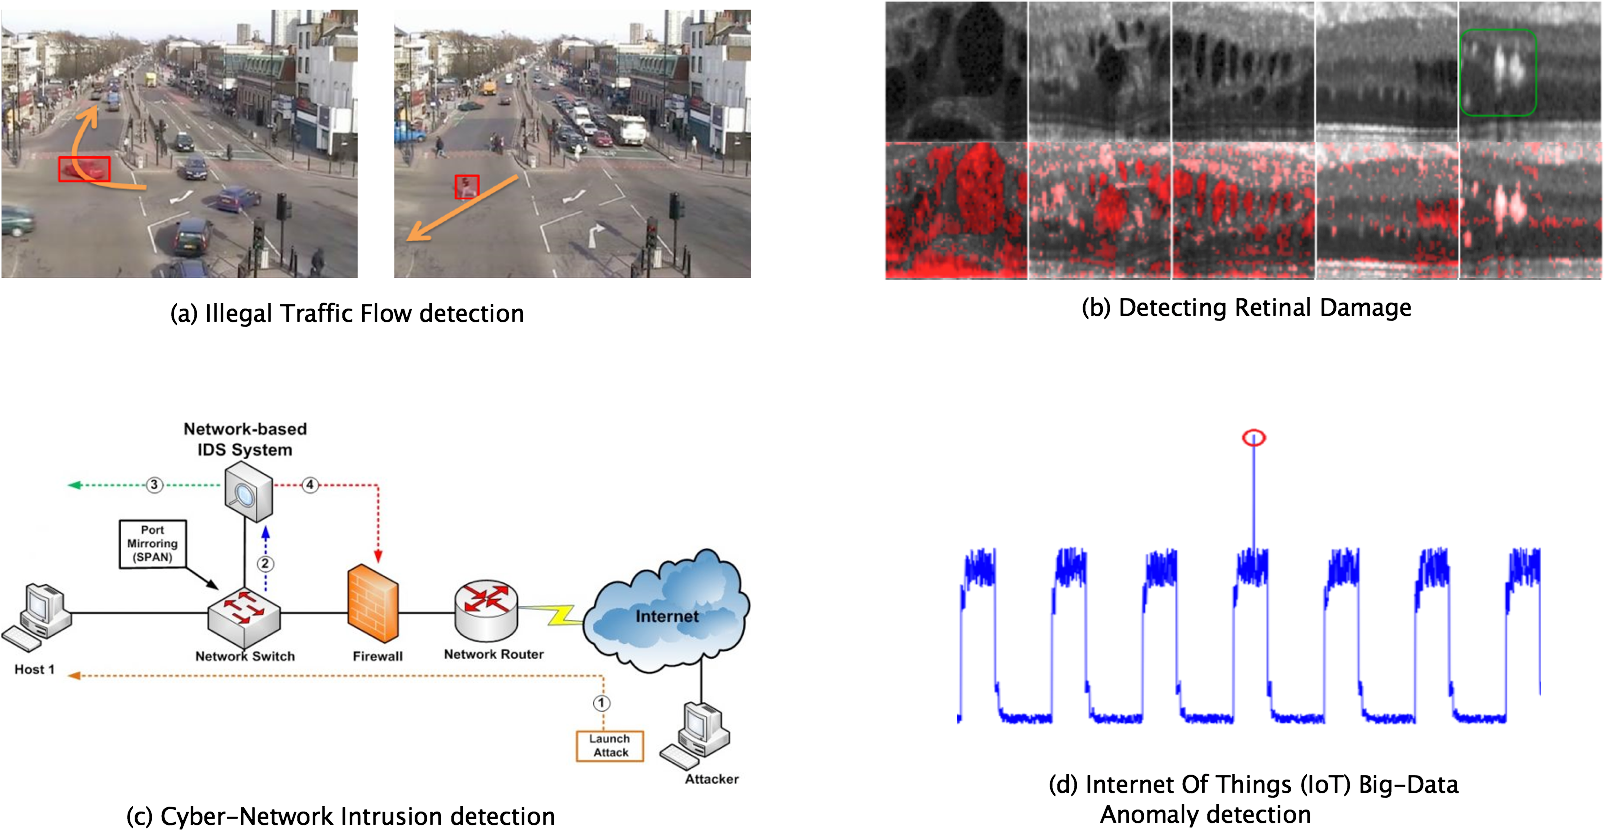
\includegraphics[scale=0.5]{images/applications}
\captionsetup{justification=centering}
\caption{Deep learning-based anomaly detection algorithms successfull applications.\\
(a) Video Surveillance, Image Analysis: Illegal Traffic detection~\cite{xie2017real},  (b) Health-care: Detecting Retinal Damage~\cite{schlegl2017unsupervised}\\
(c) Networks: Cyber-intrusion detection~\cite{javaid2016deep}  (d) Sensor Networks: Internet of Things (IoT) big-data anomaly detection~\cite{mohammadi2017deep} }
\label{fig:applications}
\end{figure}



%anomalies
\section{ What are anomalies ?}
Anomalies  are also referred to as abnormalities, deviants, or outliers in the data mining and statistics literature~\cite{aggarwal2013introduction}.
% Anomaly Detection Definition
% \begin{figure}[h]
% 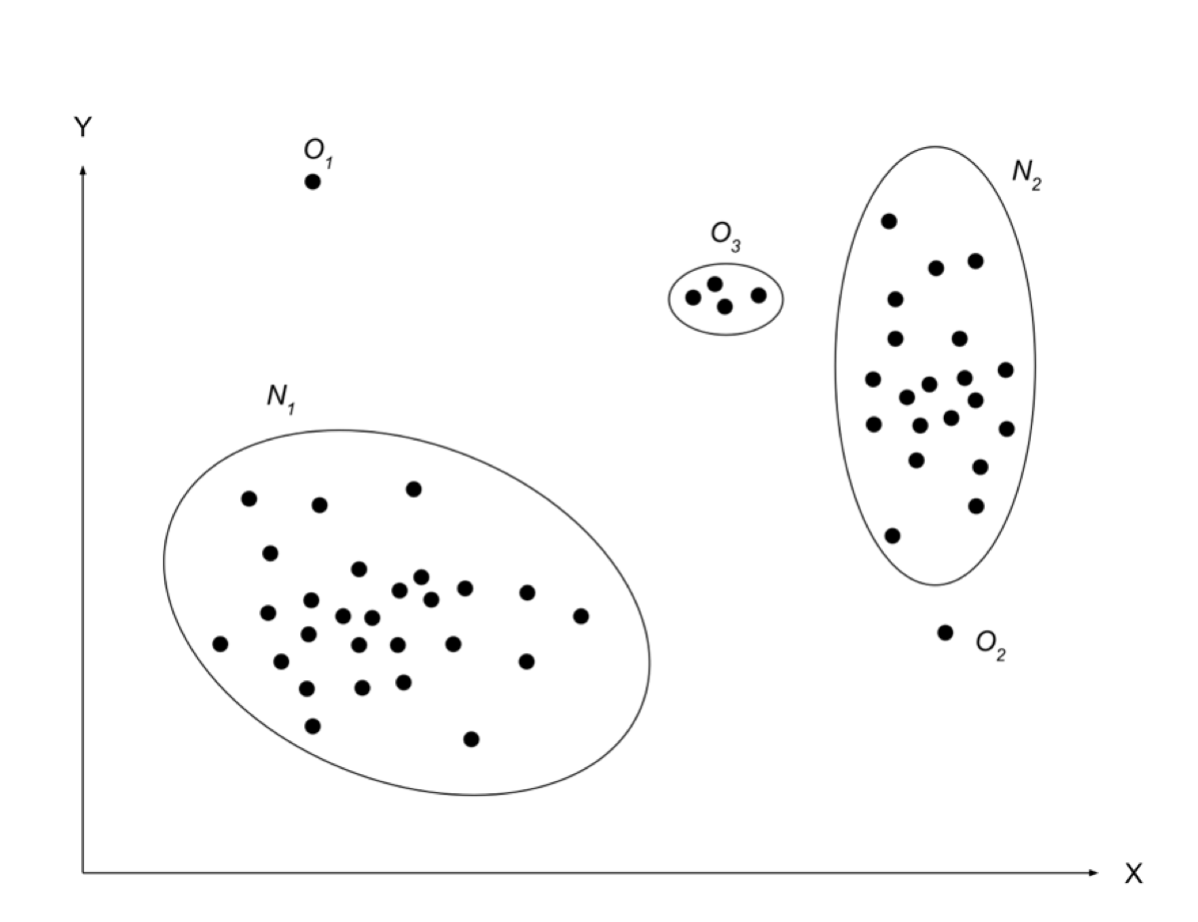
\includegraphics[scale=0.3]{images/anomalies.png}
% \caption{An illustration of anomalies in two-dimensional data set.}
% \label{fig:anomalies}
% \end{figure}

As illustrated in Figure ~\ref{fig:anomalies}, $N_{1}$ and $N_{2}$ are regions consisting of majority of observations and hence considered as normal data instance regions, whereas the region $O_{3}$, and data points  $O_{1}$ and $O_{2}$  are few data points which are located further away from the bulk of data points and hence are considered anomalies. Anomalies may arise due to several reasons, such as malicious actions, system failures, intentional fraud, etc. These anomalies reveal interesting insights about the data and are often convey valuable information about data. Therefore, anomaly detection considered an essential step in various decision-making systems.
% Novelty Detection Definition
% \begin{figure}[h]
% 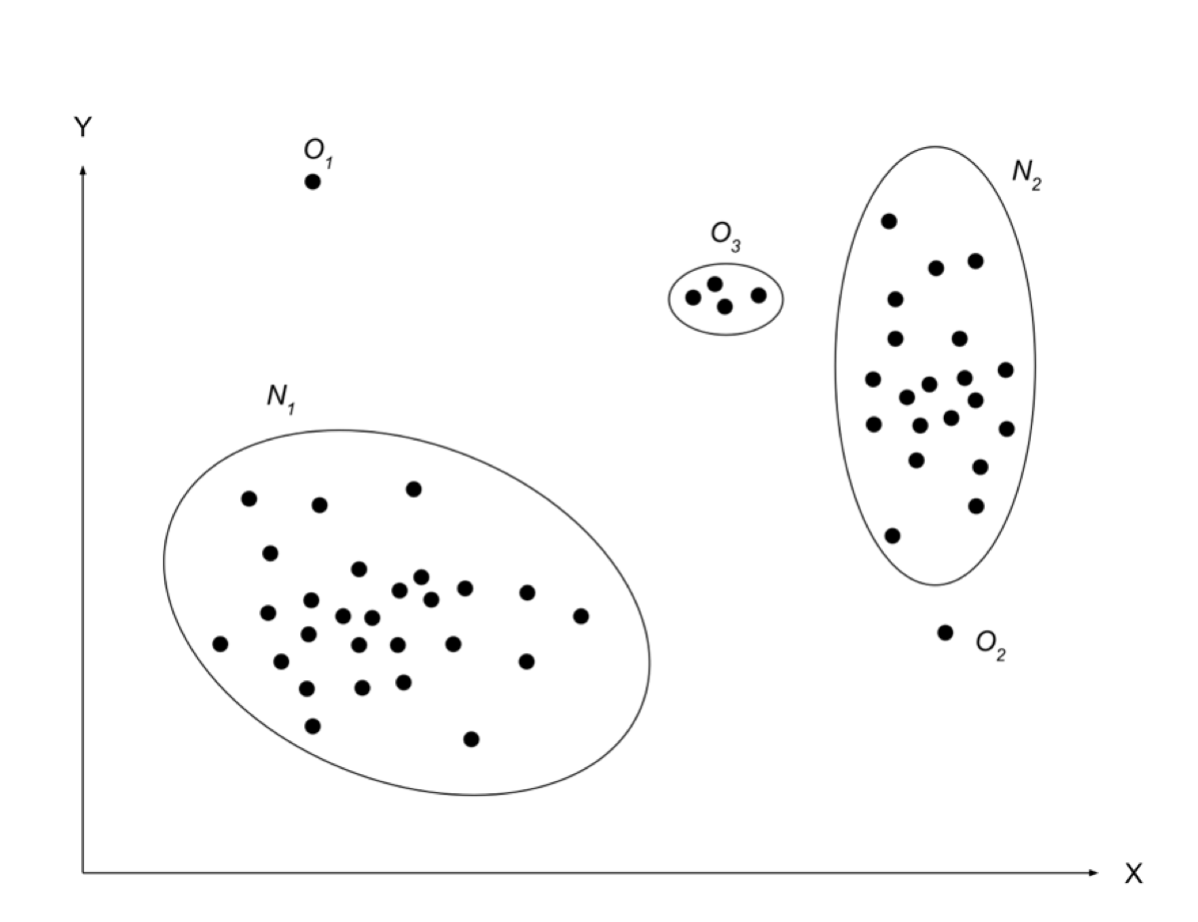
\includegraphics[scale=0.3]{images/anomalies.png}
% \caption{An illustration of anomalies in two-dimensional data set.}
% \label{fig:novelties}
% \end{figure}

% Begin of figure
\begin{figure}
  \centering
  \begin{minipage}{.48\linewidth}
    \centering
    % \subcaptionbox{}
      {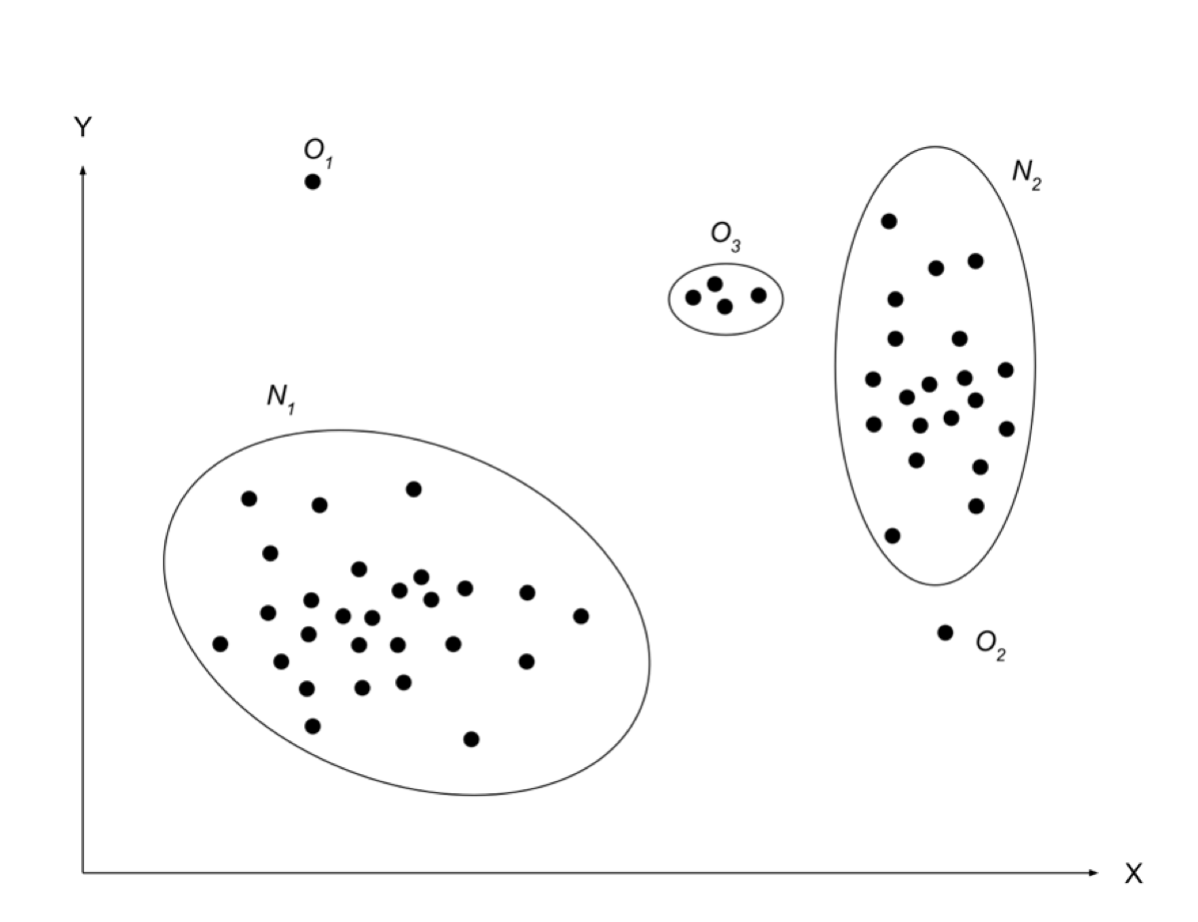
\includegraphics[scale=0.35]{images/anomalies.png}}
    \caption{Illustration of anomalies in two-dimensional data set.}
    \label{fig:anomalies}
  \end{minipage}\quad
  \begin{minipage}{.48\linewidth}
    \centering
    % \subcaptionbox{t}
      {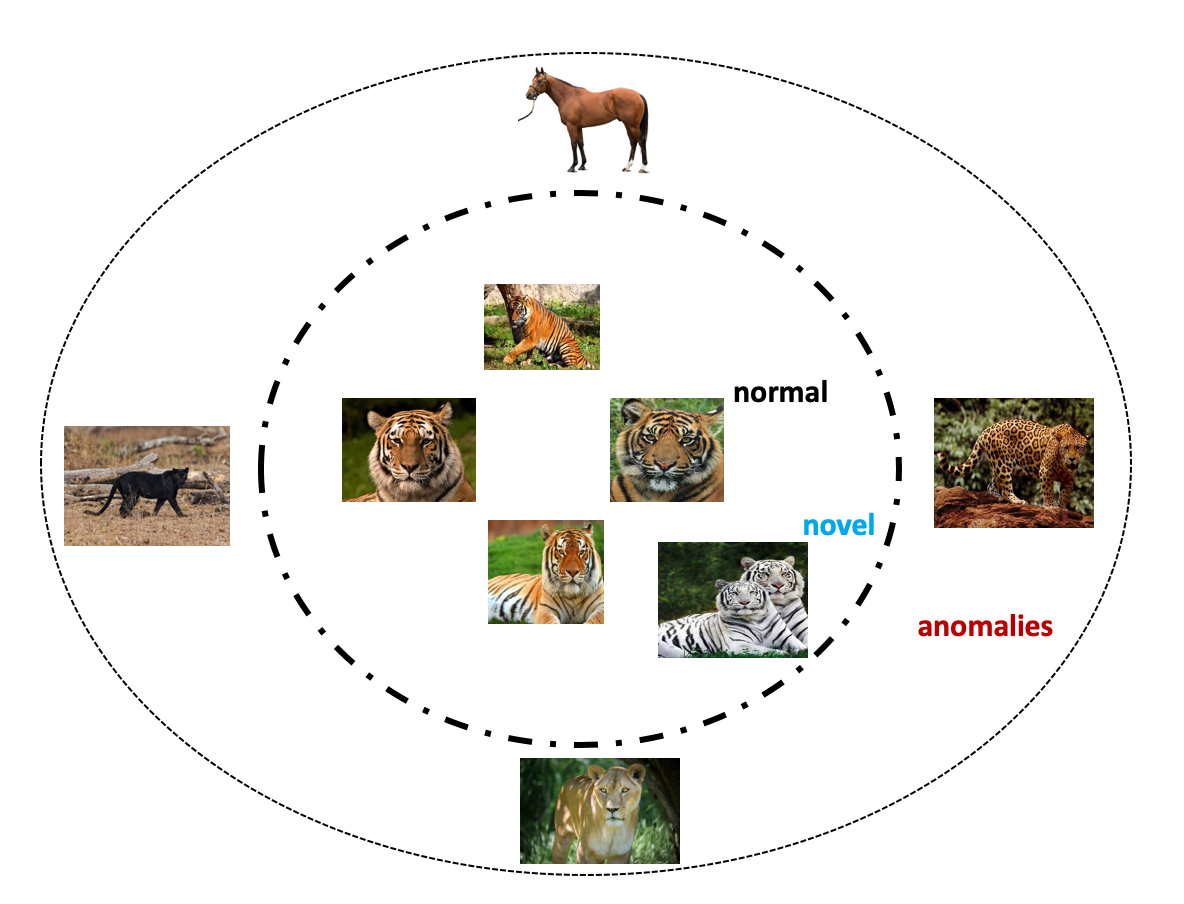
\includegraphics[scale=0.35]{images/novel.png}}
    \caption{Illustration of novelty in image data set.}
    \label{fig:novelties}
  \end{minipage}
  \bigskip

\end{figure}
% end of figure


% novelties
\section{What are novelties ?}
Novelty detection is the identification of novel (new) or unobserved patterns in the data.~\cite{miljkovic2010review}. The novelties detected are not considered as anomalous data points; instead they are incorporated into the normal data model. A novelty score may be assigned for these previously unseen data points, using a decision threshold score. ~\cite{pimentel2014review}.  The points which significantly deviate from this decision threshold may be deemed as anomalies or outliers. For instance in Figure ~\ref{fig:novelties}  the images of \textit{(white tigers)} among normal tigers may be considered as novelty, while image of \textit{(horse, panther,lion and cheetah)} are considered as anomalies.
The techniques used for anomaly detection are often used for novelty detection and vice versa.



% Challenges : Motivation and challenges Why deep learning-based anomaly detection.
\section{Motivation and Challenges: Deep anomaly detection (DAD) techniques}
\begin{itemize}
\item Performance of traditional algorithms in detecting outliers is sub-optimal on  image (e.g. medical images) and sequence data sets since they fail to capture complex structures in the data.
\item  Need for Large-scale anomaly detection : As the volume of data increases let's say to gigabytes then, it becomes nearly impossible for the traditional methods to scale to such large scale data to find outliers.
\item  Deep anomaly detection (DAD) techniques learn hierarchical discriminative features from data. This automatic feature learning capability eliminates the need of developing manual features by domain experts, therefore advocates to solve the problem end-to-end taking raw input data in domains such as text and speech recognition.
\item The boundary between normal and anomalous (erroneous) behavior is often not precisely defined  in several data domains and is constantly evolving. This lack of well defined representative normal boundary poses challenges for both conventional and deep learning-based algorithms.
\end{itemize}
% end itemize

% Begin Table
\begin{table} [ht!]
\centering
\captionsetup{justification=centering}
\caption{Comparison of our Survey to Other Related Survey Articles. \\1 \textemdash Our Survey,
2 \textemdash Kwon and Donghwoon ~\cite{kwon2017survey}, 5 \textemdash John and Derek ~\cite{ball2017comprehensive}\\
3 \textemdash Kiran  and Thomas ~\cite{kiran2018overview},            6 \textemdash Mohammadi and Al-Fuqaha ~\cite{mohammadi2017deep}\\
4 \textemdash Adewumi and Andronicus ~\cite{adewumi2017survey}       7 \textemdash Geert and  Kooi et.al ~\cite{litjens2017survey}.
}
\label{tbl:surveysummary}
\scalebox{0.75}{
\begin{tabular}{ |c|c|c|c|c|c|c|c|c|c| }
\hline
 & & 1&2&3&4&5&6&7 \\
\hline
\multirow{4}{6em}{Methods  }
&Supervised &\checkmark  & & & & & & \\
&Unsupervised &\checkmark & & & & & &  \\
&Hybrid Models & \checkmark& & & & & &  \\
&one-Class Neural Networks &\checkmark & & & & & &  \\
\hline
\multirow{8}{8em}{Applications  }
&Fraud Detection&\checkmark  & & &\checkmark & & & \\
&Cyber-Intrusion Detection&\checkmark  &\checkmark & & & & & \\
&Medical Anomaly Detection&\checkmark  & & & & & &\checkmark \\
&Sensor Networks Anomaly Detection&\checkmark  & & & &\checkmark & & \\
&Internet Of Things (IoT)
 Big-data Anomaly Detection&\checkmark  & & & & & \checkmark& \\
&Log-Anomaly Detection&\checkmark  & & & & & & \\
&Video Surveillance&\checkmark & &\checkmark  & & & & \\
&Industrial Damage Detection&\checkmark & & & & & & \\
\hline
\end{tabular}}
\end{table}
% End of Table


% Related Work
\section{Related Work}
Despite the substantial advances made by deep learning methods in many machine learning problems, there
is a relative scarcity of deep learning approaches for anomaly detection. Adewumi et.al~\cite{adewumi2017survey} provide a comprehensive survey of deep learning-based methods for fraud detection. A broad review of deep anomaly detection (DAD) techniques for cyber-intrusion detection is presented by Kwon et.al~\cite{kwon2017survey}. An extensive review of using DAD techniques in medical domain has been presented by Litjens et.al ~\cite{litjens2017survey}. An  overview of DAD techniques for Internet of Things (IoT) and  big-data anomaly detection is introduced by  Mohammadi et.al~\cite{mohammadi2017deep}. Sensor networks anomaly detection has been reviewed  by  Ball et.al~\cite{ball2017comprehensive}. The state-of-the-art deep learning based methods for video anomaly detection along with various categories has been presented in~\cite{kiran2018overview}. Although there are a number of reviews in applying DAD techniques, there is shortage of comparative analysis of deep learning architecture adopted for outlier detection. For instance a substantial amount of research on anomaly detection is conducted using deep autoencoders, but there is lack of comprehensive survey of various deep architecture's best suited for a given data-set and application domain. We hope that this survey bridges this gap and provides a comprehensive reference for researchers and engineers aspiring to leverage deep learning for anomaly detection. Table~\ref{tbl:surveysummary} shows the set of research methods and application domains covered by our survey.

% The classification taxonomy is also present in this paper $https://www.ncbi.nlm.nih.gov/pmc/articles/PMC4836738/$
% This paper~\cite{erfani2016high} presents a hybrid approach of combining deep learning models in combination with other traditional techniques to identify outliers and obtained promising results.

% Anomaly Detection Taxonomy
\begin{figure}[h]
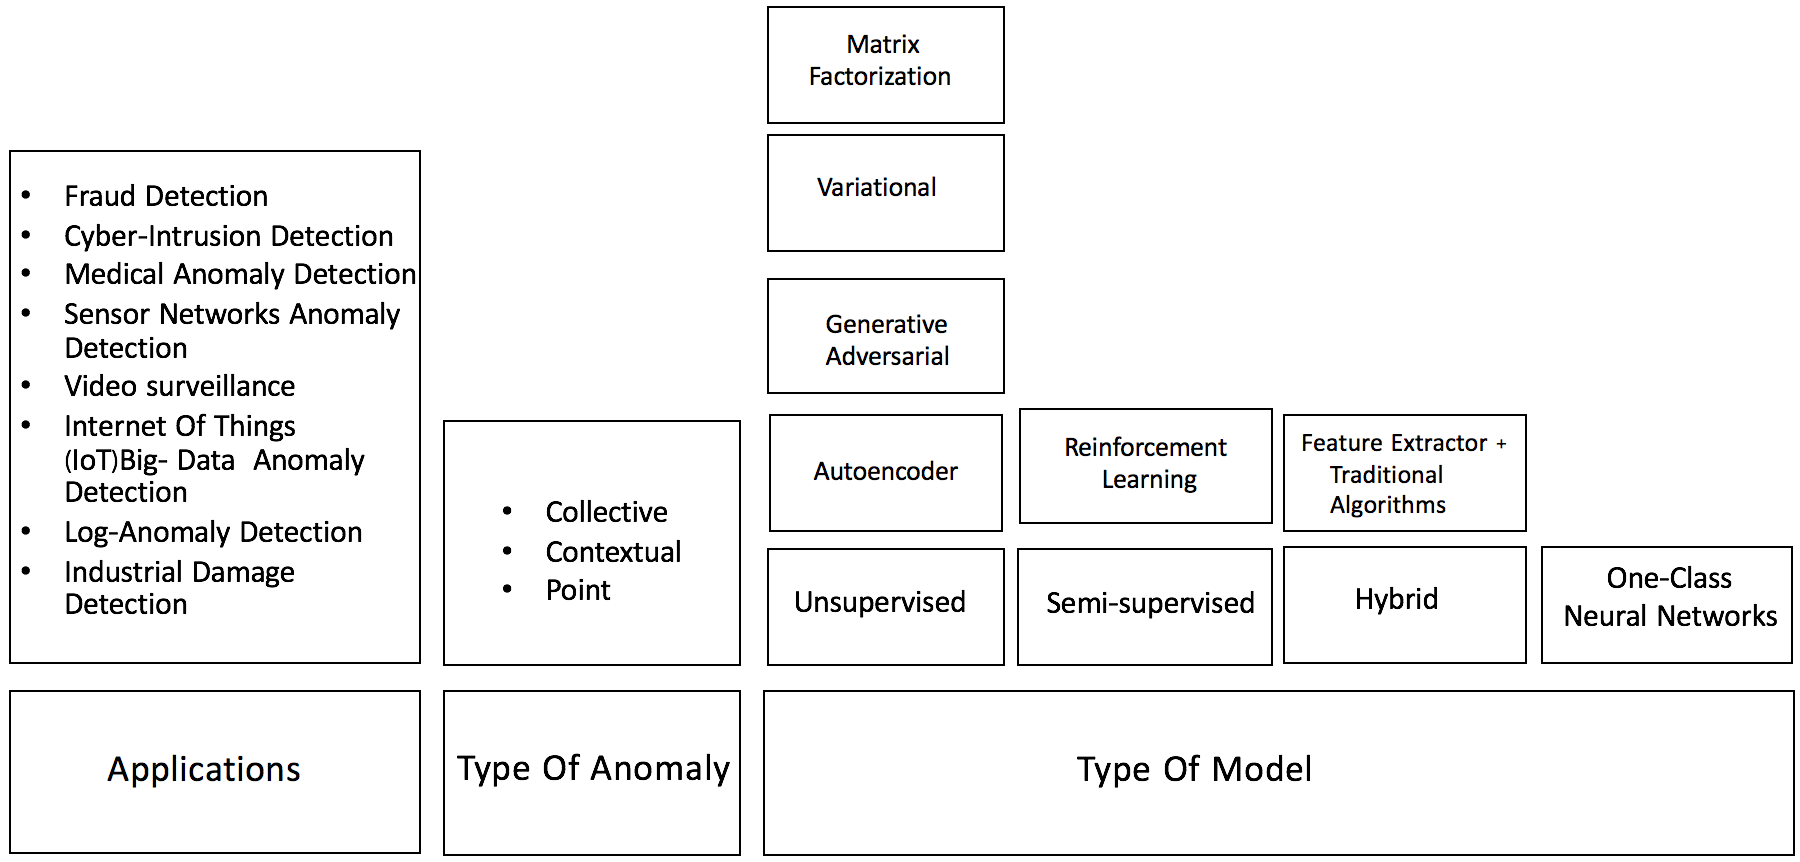
\includegraphics[scale=0.45]{images/AnomalyDetectionTaxonomy}
\caption{Key components associated with deep learning-based anomaly detection technique.}
\label{fig:surveyTaxonomy}
\end{figure}
% end of related work

%% Our Contributions
\section{ Our Contributions}
We follow survey approach of V.Chandola and A.Banerjee et.al~\cite{chandola2007outlier} for deep  anomaly detection (DAD). Our survey presents a detailed and structured overview of research and applications of DAD techniques. We summarize our main contributions as follows:
\begin{itemize}
\item Most of the existing surveys on DAD techniques either focus on a particular
application domain or specific research area of interest~\cite{kiran2018overview,mohammadi2017deep,litjens2017survey,kwon2017survey,adewumi2017survey,ball2017comprehensive}.
This review aims to provide a comprehensive outline of state-of-the art research in DAD techniques as well as several real world applications these techniques are discussed.
\item In recent years a number of new deep learning based anomaly detection techniques  with greatly reduced computational requirements have been developed. The purpose of this paper is to survey these techniques and classify them into organized schema for better understanding. We introduce two more sub-categories Hybrid models ~\cite{erfani2016high} and one-class neural networks techniques~\cite{chalapathy2018anomaly} as illustrated in Figure~\ref{fig:surveyTaxonomy} based on the choice of training objective. For each categories we discuss both the assumptions and techniques adopted for best performance. Furthermore within each category, we also present the challenges, advantages and disadvantages and provide an overview of computational complexity of DAD methods.
\end{itemize}

% Organization of the paper
\section{Organization}
This chapter is organized by following structure described in Figure~\ref{fig:surveyTaxonomy}.
In Section~\ref{sec:aspectsOfAnomalyDetection}, we identify the various aspects that determine the formulation of the problem and highlight the richness and complexity associated with anomaly detection.
We introduce and define two types of models: contextual and collective or group anomalies. In Section~\ref{sec:applicationsOfDLAD}, we briefly describe the different application domains to which deep learning-based anomaly detection has been applied. In subsequent sections we provide a categorization of deep learning-based techniques based on the research area to which they belong.  Based on training objectives employed and availability of labels  deep learning-based anomaly detection techniques  can be categorized into supervised (Section~\ref{sec:supervisedDAD}), unsupervised (Section ~\ref{sec:unsupervisedDAD}), hybrid (Section~\ref{sec:hybridModels}), and one-class neural network  (Section~\ref{sec:oneclassNN}). For each category of techniques we also discuss their computational complexity for training and testing phases. In Section~\ref{sec:typeBasedAD} we discuss  point, contextual, and collective (group) deep learning-based anomaly detection techniques. We present some discussion of the limitations and relative performance of various existing techniques in Section~\ref{sec:relativeSOW}. Section~\ref{sec:chapter1_conclusion} contains concluding remarks.

% \titlespacing{\section}{0pt}{2ex}{1ex}

\section{Different aspects of deep learning-based anomaly detection. }
\label{sec:aspectsOfAnomalyDetection}
This section identifies and discusses the different aspects of deep learning-based anomaly detection.

%%%%%%%%%%%%%%%%%%%%%%%% Begin of  Nature of Input data %%%%%%%%%%%%%%%%%%%%%%%%
\subsection{ Nature of Input Data}
The choice of deep neural network architecture in deep anomaly detection methods primarily depends on the nature of input data. Input data can be broadly classified into sequential (eg, voice, text, music, time series, protein sequences) or non-sequential data (eg, images, other data). Table~\ref{tab:dataTypeModelArchitecture} illustrates the nature of input data and deep model architectures used in anomaly detection. Additionally input data depending on the number of features (or attributes) can be further classified into either low or high-dimensional data. DAD techniques have been to learn complex hierarchical feature relations within high-dimensional raw input data ~\cite{lecun2015deep}. The number of layers used in DAD techniques is driven by input data dimension, deeper networks are shown to produce better performance on high dimensional data. Later on in the Section ~\ref{sec:deepDADModels}  various models considered for outlier detection are reviewed at depth.
 
\input{Problem}
\section{ General Framework for Group Deviation Detection
}
 \label{Sec:Framework}
In the last section, we clearly defined the problem of detecting group deviations in static and dynamic situations.   
  This section elaborates  upon the general framework and underlying structure for GAD and GCD techniques. Discovering significant group deviations is related to three sub-problems. 
\begin{enumerate}[1.]
\item {\it Group Structures}:  The definition of groups and the relationship between data instances is important to understand. %  clustering algorithm aggregate data instances into group structures.
\item {\it Statistical Properties}:  
A variety of statistical properties may characterise group deviations. % For example, a user is able to examine statistical properties of interest such as proportions, location or dependence.
 If statistical properties  are  not adequately quantified then relevant group deviations cannot be identified.
\item  {\it Model Design}: 
 The design of GAD and GCD techniques include data inputs,   model assumptions, learning approaches and output information. 
\end{enumerate}


\subsection{Group Structures}
We now highlight examples of different problems associated with group structures.   A group is a collection of two or more related data instances where Tan et al.  \cite{Tan} state that a data instance is synonymous with terms such as  vector, sample, entity, observation, etc. %Many GAD techniques assume that features from members in a group are independent and identically distributed (iid) where
Members in a group can be related by  external information of known group labels such as in topic modelling where Xiong et al. \cite{FGM} consider a document as a group of  words or a corpus as a group of documents. When group structures are not previously known, clustering algorithm aggregate data instances based on similarity criterion. 
 For example, Xiong et al. \cite{MGM} infer a spatial cluster of galaxies with distances closer than 1 megaparsecs while Wong et al. \cite{wong-rule} examine a demographic group of patients  based on certain categorical features.  
%   The interpretation of results relies on initial definition and construction of group structures. 
  
When group structures are unknown a priori,  clustering algorithms are applied. Common procedures minimise the cumulative  distance  between  members in a group to a central reference point. %These algorithms such as $k$-means or  nearest neighbors
 Clustering algorithm  for numerical values  are discussed in Jain \cite{jain2010} where a group of data instances contains members with similar features based on minimising distance metrics.   
Steinbach \cite{steinbach2004} discusses issues with distance-based clustering algorithms as data points become difficult to differentiate in higher dimensions.   More sophisticated techniques have been specifically developed for group  
%In particular,
 group deviation detection   %techniques infer clusters based on different criterion 
 such as:
\begin{enumerate}[-]
\item Chen et al.  \cite{GLETS}  apply density-based spatial clustering based on Pearson's correlation and Euclidean distance between values of times series. 
%\item Chen et al.  \cite{Chen2014} examine Pearson's correlation and Euclidean distance between values of times series.  
\item    Yu et al. \cite{GLAD} examine individual features as well as pairwise connection data.  %infer groups containing a mixture of social roles for social media applications. 
\item Soleimani and   Miller \cite{ATD} infer anomalous clusters of documents based on likelihood probabilities.
\item Dai et al. \cite{ERACD} cluster based on the ranking of feature values. 
\end{enumerate}
Therefore there are many procedures for clustering data instances when group structures are previously unknown.


\begin{figure}[h]
\centering
   \begin{subfigure}{1\linewidth} \centering
     \includegraphics[width=6cm, height=4cm,trim=5cm 9.5cm 4.5cm 9cm]{FIGURES/ECGa}
     \caption{A collective anomaly (red dotted circle) in the ECG reading of a single patient.}
   \end{subfigure}
   \begin{subfigure}{1\linewidth} \centering
     \includegraphics[width=6cm,  height=4cm,trim=5cm 9.5cm 4.5cm 8.5cm]{FIGURES/ECG}
     \caption{A group anomaly (Patient 3) is observed when comparing several patients.} 
   \end{subfigure}
  % \vspace{-1cm}
\caption{ In (a), a collective anomaly is a collection of related data instances that is anomalous with respect to time-dependent observations from  a single patient.   
In (b), a group anomaly is a specific example of a collective anomaly where  the entire dataset involves a group of observations from multiple patients. 
 } \label{Fig:ECG}
\end{figure}
%\vspace{1cm}


 
 
In our thesis, we do not use group anomaly and  collective anomaly interchangeably.  Chandola \cite{Chandola} defines a collective anomaly  as "a collection of related data instances that is anomalous with respect to the entire dataset." 
A group anomaly is specific example of a collective anomaly where  
the entire dataset involves multiple groups. % in the dataset. 
To differentiate these terms, consider the electrocardiogram (ECG) example from Goldberger et al. \cite{Goldberger}.  Figure \ref{Fig:ECG} (a) highlights a collective anomaly (in the dotted red circle) that exhibits an irregular pattern as compared to the  entire dataset (time series of a single patient). For a GAD application,  Figure \ref{Fig:ECG} (b) illustrates ECG readings from several patients  where  Patient 3 represents a group anomaly as the statistical properties are significantly different.  %however this is also a collective anomaly as the entire dataset can be considered as information from all of the patients.
 A realistic GCD case  would involve a group of patients with ECG readings similar to Figure \ref{Fig:ECG} (a) where a large-scale phenomena affects all patients around $\tau=10$. 
 


\subsection{Statistical Properties}
% SP - known vs unknown
 In some cases, a domain expert is interested in particular  statistical properties of groups. Statistical properties are measured and compared for group deviation detection. In terms of point-based and distributed-based group behaviours, point-based group deviations are characterised by a central location while distributed-based group deviations are characterised by statistical properties other than location such as scale, shape or dependence. In practice, group deviations are difficult to detect as a combination of statistical properties may  significantly differ. If a user is able to specify statistical properties of interest, group deviations are more easily detected and interpreted. 

 Since there are also many ways to quantify statistical properties of groups, we describe common parametric and non-parametric measures for statistical properties in Table \ref{Tab:Des} where non-parametric measurements are more robust to individual outliers. %Statistical properties in Table \ref{Tab:Des}, capture group  behaviours  for continuous variables however other metrics are more suitable for discrete or categorical datasets. 
   Given prior knowledge of statistical properties that characterise group deviations for GAD or GCD applications, a suitable method for discriminating groups is easily constructed. However when the nature of significant group deviations in terms of statistical properties is unknown, more   specialised techniques are required.  
 
 
		\begin{table}[h]
%\renewcommand{\arraystretch}{1}
	\tabcolsep=0.1cm
	\begin{center}
   \scalebox{0.88}{
	\begin{tabular}{lccc  }
	\hline\\[-2mm]
		%\multirow{ 2}{*}{} & & & \\[2mm]
 Statistical & %Function &
	 Parametric Measures% in $\boldsymbol \alpha$ 
	 &  Non-parametric Measures %  in  $\boldsymbol \gamma$ 
	 \\[-1mm]  Property & & &
	 \\[2mm] \hline\\[-2mm]
		\multirow{ 2}{*}{Location } & %	\multirow{ 2}{*}{$h_1$ }&
	  $ \displaystyle\bar{ {X}}_v=\frac{1}{N} \sum_{n=1}^N X_{nv}$ & $  \displaystyle \hat{q}_v({0.5})$  \\
	 & \hspace{5mm}(mean) & (median)  \\%[2mm]
	  %
	\multirow{ 2}{*}{Scale} & %\multirow{ 2}{*}{$h_2$} &
	 $ \hat\sigma^2_v = \displaystyle	\frac{1}{N-1}\sum_{n=1}^{N} \big(X_{nv}-\bar {X}_v \big)^2$  &  % \displaystyle s^2 =	\(\stackunder[1pt]{$ \mbox{mediai}$}{	\scalebox{0.8}{$ 1\le i\le N$}} \) $\big (| X_n - q_{0.5}| \big)$ 
	$\displaystyle \hat{q}_v({0.75}) - \hat{q}_v({0.25})$ \\ %[-1mm]
	 & (variance) &(interquartile range)   \\[1mm]
	 Skewness & % $h_3$ &
	$\displaystyle\frac{1}{N} \sum_{n=1}^N \frac{( X_{nv}-\bar{X}_v)^3}{ \hat\sigma_v^3}  $  & 
	$ \displaystyle \frac{\hat{q}_v({0.9}) + \hat{q}_v({0.1}) -2 \hat{q}_v({0.5}) }{  \hat{q}_v({0.9}) - \hat{q}_v({0.1})  }$\\[4mm] %\displaystyle  \hat{\mathcal{S}}=
	 Kurtosis &  %$h_4$ &
	 $\displaystyle\frac{1}{N} \sum_{n=1}^N \frac{( X_{nv}-\bar{X}_v)^4}{ \hat\sigma_v^4}  $ &
	$ \displaystyle\frac{\hat{q}_v({0.975}) -\hat{q}_v({0.025}) }{\hat{q}_v({0.75}) -\hat{q}_v({0.25}) }  $ \\[4mm] %\displaystyle \hat{\kappa} =
	 	\multirow{ 2}{*}{Dependence} &  	%\multirow{ 2}{*}{$H$} &
	  $ \; %\hat \rho =
	   \displaystyle\frac{ \sum_{n} \big(X_{n1}- \bar X_{1} \big) \big(X_{n2} - \bar X_{2}\big) } {\sqrt{ \sum_n \big(X_{n1}- \bar X_{1} \big) ^2 \sum_n \big(X_{n2} - \bar X_{2}\big)^2 }   } $ & 
	\;\; $\displaystyle   \frac{ \sum_{n} \big(R_{n1} - \bar R_{1} \big) \big(R_{n2} - \bar R_{2}\big) } { \sqrt{ \sum_n \big(R_{n1} - \bar R_{1} \big) ^2 \sum_n \big(R_{n2} - \bar R_{2}\big)^2  }} $ \\
	 & (Pearson's correlation ) & (Spearman's rank correlation \cite{Spearman})\\[1mm] % \hat{\rho} = 
	 \hline\\[-2mm]
	 \end{tabular}
	 }
	\end{center}
	\caption{ Given a group ${\bf G} =(X_{nv})  \in \mathbb{R}^{ N \times V}$,  the $\beta$-quantile  $\hat{q}_v(\beta)$ is estimated from  the empirical distribution of the $v$th column of random variables. Also
$R_{\cdot v}  \in \mathbb{R}^{ N }$  denotes ranked values  of $X_{\cdot v}$ with average column rank $\bar R_v$.  % Note Pearson's correlation captures a linear relationship between variables whereas Spearman's rank correlation \cite{Spearman}  measures a monotonic (possibly non-linear) dependence.
Non-parametric measures of skewness and kurtosis are respectively described in 
Hinkley   \cite{hinkley1975} 
and Moors \cite{RobustK}.
}
 \label{Tab:Des}
\end{table}  
 
% SP - characterise, measure 
In most applications, statistical properties that characterises group deviations are usually known. Without prior information, it is difficult to differentiate a group deviation  as there may be a significant difference in a combination of statistical properties. %Also if an incorrect selection of statistical properties are analysed then significant group deviations cannot be identified. 
  Guevara et al. \cite{SMDD} explore the GAD application and find that more complicated group behaviours are not adequately characterised by single quantities such as location estimates of group distributions. %Their study investigates examples of Gaussian mixtures where a group anomaly is generated from a different proportion of distributions.
 % Another issue occurs for high dimensional datasets as common measures of statistical properties in Table \ref{Tab:Des} may not properly characterise the behaviour of groups.
   Topic models are applied for GAD problems  where  statistical properties of  groups represent  proportions of inferred topic  variables.  % high number of dimensions where  models extract . 
  We  discuss topic models in more detail for  GAD applications in Chapter \ref{sec:staticGAD}.   



\subsection{Model Design} 
After understanding problems associated with group structures and statistical properties of interest, a domain expert can construct suitable solutions for GAD and GCD problems. Firstly models are designed to be compatible for specific types of input data such as continuous or categorical variables. To appropriately identify group deviations, discriminative methods do not impose data assumptions  while generative models assume how data is generated.  Given availability of labeled group behaviours, models either apply  supervised or unsupervised learning. Another important aspect of model design is  interpreting outputs with scores or labels.  The model design of group deviation detection techniques requires a clear understanding. 

\subsubsection{Input Data }
Certain models are compatible for specific types of input data.   As specified by Equation (\ref{Eqn:Domain}) in the problem definition, data types that are explored in GAD and GCD applications include  discrete, continuous or categorical features.
Data types also influence the appropriateness of statistical properties for characterising  groups behaviours. In particular, generative models are flexible in assuming a Gaussian distribution for continuous real-valued data whereas categorical features are modelled by categorical distributions.   
 Pairwise network connections are also a possible type of input data and are usually  incorporated for clustering when group structures are previously unknown.  Similarly, certain clustering algorithms are only compatible for specific data types. 


 
\subsubsection{Assumptions}
 The assumptions of GAD and GCD techniques  are  discussed in terms of discriminative and generative models.  %where supervised or   unsupervised learning is applied depending on the availability of labeled data.  
Discriminative approaches are useful for directly classifying groups into regular and anomalous behaviours without knowledge of how data is generated.  %Due to the lack of regular and anomalous group labels, discriminative GAD techniques classify regular behaviour based on the predominant group pattern.  
 On the other hand, generative models assume specific probability density functions over   variables.  Hypothesis tests are a special type of generative model that further classify group deviations. %GAD and GCD  techniques  are classified as either  discriminative or generative models however hypothesis tests are also elaborated on.  
% Common advantages and disadvantages of 
Table \ref{Tab:DG} lists common advantages of  discriminative methods, generative models as well as hypothesis tests. % for  GAD and GCD  applications. 

\begin{table}[H]
	\tabcolsep=0.3cm
	\renewcommand{\arraystretch}{1.2}
	\begin{center}\scalebox{1}{
	\begin{tabular}{lcccccccccccccccc  }
	\hline\\[-6mm]
 Procedure & $\mathcal{A}1$ & $\mathcal{A}2$ & $\mathcal{A}3$ & $\mathcal{A}4$ & $\mathcal{A}5$  \\[-1mm] \hline \\[-8mm] \hline\\[-6mm]
  Discriminative Methods   & \yeah & \nope & \yeah  & \nope & \nope \\
  Generative Models   & \nope & \yeah & \nope  & \yeah & \nope \\
 Hypothesis Tests  & \yeah & \yeah & \nope  & \yeah & \yeah\\[3mm]
\hline 
	 \end{tabular}
	}
	\end{center}
	\medskip
		\caption{  Summary of advantages of   group deviation detection techniques in terms of 	 discriminative methods, generative models and hypothesis tests. If a procedure has a particular advantage, a tick label is present whereas if a procedure lacks an advantage, a cross is displayed.  }
	%\vspace{-5mm}
 \label{Tab:DG}
\end{table}  

	
	
\begin{enumerate}[{$\mathcal{A}$}1] \setlength\itemsep{5pt}
\item   {\it Direct classification}:  discriminative models and hypothesis tests provide explicit boundaries between regular   behaviours and significant group deviations. 
 \item  {\it Rich Interpretation}: Results from discriminative methods  are difficult to interpret due to the complex representation between group   variables. For explanatory purposes, 
  generative models offer a rich interpretation of  groups and inferred statistical properties.    The flexible structure of generative models is also useful for incorporating prior information.
  \item  {\it  Minimal  Assumptions}: 
  Discriminative approaches assume that group behaviours can be differentiated based on certain optimisation criteria.   Generative models further impose distributional assumptions which are not  appropriate for all datasets. 
  \item  {\it Prevents Overfitting}: Discriminative methods are prone to overfitting model parameters especially on  training data with smaller sample sizes. 
 Generally, generative models experience less overfitting  when the model assumptions are appropriate for given datasets.  
   \item  {\it Statistical Significance}: In addition,  hypothesis tests determine whether the statistical properties of a group is significantly different. In many cases, generative models arbitrarily classify    significant group deviations based on highest anomalous scores. 
\end{enumerate}	




\subsubsection{Learning}
Supervised learning requires previously labelled group behaviours while  
unsupervised approaches learn the dominant pattern in the dataset. 
When surveying current state-of-the-art group deviation detection 
 techniques, most discriminative  and generative models employ unsupervised learning.  
 Unsupervised learning is preferred as  ground truth labels of regular or irregular behaviours are not usually available. In a  comparison study conducted by Laskov et al. \cite{laskov2005learning},  unsupervised methods achieve a higher accuracy than  supervised algorithms when learned behaviours from a training data do not account for unknown patterns in a test set.  Unsupervised methods are beneficial for  discovering novel group patterns. 

\subsubsection{Output}
The output from group deviation detection techniques  is given by classification labels or  scores indicating significant group deviations.  
 Discriminative methods produce binary labels for regular or anomalous classes in GAD while GCD methods estimate times of significant change in a dynamic group over time.   Generative models  tend to compute scores that quantifies the degree that a  group is significantly different as compared to other groups in a dataset. Scores from generative models are often converted to a classification by a threshold chosen by a user however  this selection is subjective and equivocal.  Hypothesis tests are advantageous for obtaining classification labels based on the statistical significance of group deviations.  
  

  




\section{Challenges}
We now discuss challenges associated with group deviation detection. There are many issues that arise from inadequate group definitions in a dataset. Datasets involving group structures are more difficult to understand and analyse than many pointwise data problems with potential absence of group labels. Benchmark datasets are currently unavailable and thus comparison studies are difficult to conduct. Even though detecting group deviations may seem like a straightforward task, results require validation and careful interpretation. The challenges in  GAD and GCD applications  include:

\begin{enumerate}[\textbullet]
\item {\it  Defining Groups}:
 F\~{a}rber et al. \cite{ClusterEval}   highlight that known group labels may not represent natural clustering patterns in a dataset. 
 However when group memberships are unknown a priori,   clustering method possibly lead to inadequate group representations. Group structures  may be improved by incorporating additional information such as known regular group behaviour or pairwise relationships between data instances. 
 \item {\it Defining Group Deviations}: Group deviations can be defined based on the number of groups or the number of  data instances within groups. Usually when groups possess similar sizes, group deviations occur as a minority of group observations.    
  % Consider  a single group that contains more observations than the total number of other groups. 
\item {\it Capturing Statistical Properties}: Group deviations may occur in a variety of statistical properties such as location, scale, shape, etc.    Borgatti et al. \cite{GroupSocialMedia} explain that more complicated patterns exist when each member contributes to behaviour of a group. Thus an effective detection method has to adequately capture properties of groups in order to identify significant deviations.
% \item {\it Evolving Patterns}: In many domains, the notion and definition of group deviations also changes over a period of time. Algorithms that can adapt to identifying evolving unknown group patterns  are preferable in many applications. 
\item {\it Not statistically significant}: Many methods classify or score group behaviours however they do not quantify statistical significance. In many cases, it is difficult to distinguish noisy group observations from a significant group deviation. 
\item {\it Absence of Group Labels}: When group memberships are unknown a priori, clustering  induces additional uncertainty in analysis and subsequent results. Halkidi et al. \cite{ClusterValidity} explain that it is also difficult to evaluate the effectiveness of inferred clusters without sufficient ground truth labels. 
\item {\it Absence of Ground Truth Labels}: Like other anomaly detection applications, ground truth labels are usually unavailable. To investigate group deviations rather than a single  instance, requires more time and effort for obtaining  ground truth labels.  
\item {\it Absence of Benchmark Datasets}: Since there is a lack of benchmark group datasets, many methods resort to anomaly injection. Anomaly injection involves contaminating a real-world dataset with significant deviations and subsequently comparing detected instances with  ground truth labels. This does not account for  anomalies that are naturally present in a dataset such that injected anomalies should possess higher deviations than naturally occurring anomalies. 
\item {\it Absence of Robust Comparison Studies}: Evaluative metrics that assess  group deviation detection datasets would be useful for a robust comparison study. For pointwise anomaly detection methods, Campos et al. \cite{Campos2016} propose two measures for a dataset; difficulty of detecting different types of anomalies and diversity or agreement between scores computed from methods.  A similar evaluative process is recommended for group deviation datasets to provide a more robust comparison of state-of-the-art techniques. 
\end{enumerate}
There is no single solution that overcomes all of these challenges in GAD and GCD research.  We further elaborate on related work for group deviation detection techniques in static and dynamic scenarios. 


\section{Related Work}
Due to continual research involving  anomaly detection and change detection,  there are additional problems and  techniques that are proposed after the publication of many papers. Extensive reviews on pointwise anomaly detection techniques are conducted by Hodge and  Austin \cite{Hodge}  as well as Chandola et al. \cite{Chandola}.   Since change detection is a general topic, many techniques are domain specific where  
Singh \cite{singh1989review} examines the application to remote sensor data while Reeves et al. \cite{reeves2007review} explore change detection techniques for climate data. An overview of temporal outlier detection is provided by Gupta et al. \cite{Gupta2013}. Many of these papers  briefly discuss  group applications however GAD and GCD are emerging areas of research where most state-of-the-art techniques have been more recently developed.  Yu et al. \cite{SurveySocialMedia} and  Xiong \cite{Collective}  provide descriptions of current state-of-the-art GAD methods.  % 

{  
GAD is closely related to zero-shot learning (ZSL) where data instances are classified however their behaviour may not be seen in training. % different classes even when unseen instances in a test set   that are not present in the training set.
%There is an overlap between GAD and zero-shot learning (ZSL) techniques however there are fundamental difference. 
Surveys on ZSL have been conducted by Xian et al. \cite{ZSLsurvey} where ZSL assumes a subset of classes (groups) are known during training whereas GAD techniques are more general as none of regular  group behaviours (classes) may be available.
%GAD is more general than ZSL as classes (groups) may not be available while ZSL assume classes are known during training.     
 %ZSL accounts for the simple case where training and test set are disjoint while classes in  training and test set may overlap for generalised ZSL. 
  Without known classes,  Kodirov et al. \cite{unsupervisedZSL} propose an unsupervised ZSL technique that incorporates auxiliary textual information.   ZSL techniques are specfically formulated for certain domains such as image classification \cite{ZSLanomaly} and network intrusion  \cite{perez2016} however we focus on GAD techniques that are applicable for more general domains. 



%Group change detection  
Similarly the GCD problem has been  specifically formulated for many real-world applications. In video change detection, a video can be modelled as a group of color pixels or visual features where  significant deviations in video frames are detected over time. Lienhart 
\cite{VideoSurvey} provides a survey of video transition (gradual change) detection techniques while a comparison study of performance for video-shot-change (abrupt  change) detection algorithms is conducted in Gargi et al. \cite{gargi2000}. %Other methods such as  Yuan et al. \cite{yuan2017anomaly} identify subtle changes in  traffic scenes while  %Yuan et  al.   \cite{yuan2016hyperspectral} examine  reflectance spectrum data.
%Rout et al. \cite{rout2018}  detect changing  positions of dynamic objects in an underwater video.
  In other applications, Sakaki et al. \cite{sakaki2010} detect an earthquake event by monitoring a group of keywords on Twitter and  Xie et al. \cite{xie2013} explore  sequential change-point detection in multiple sensor readings over time. % the average value of  sensor readings over time. % and also estimate the affected proportion  of sensors at a specific time step.  
Many of these GCD techniques are only applicable in  specific domains and are not flexible for detecting changes in a variety of statistical properties.   
}

 
\section{Group Anomaly Detection (GAD) Techniques} \label{Sec:D}
% Brief paragraph 
After setting up the group deviation detection  problem and describing the general framework for methods in previous sections, we now  explain specific GAD techniques in further detail. A description of GAD techniques is provided in terms of the four key components from Section   \ref{Sec:Problem}.  GAD involves comparing multiple groups and identifying groups with significantly different statistical properties.   GAD methods fall into  categories of discriminative methods and generative models. Hypothesis tests are a specific generative models that also described in the following.  



\subsection{ GAD Discriminative Methods } 
 In GAD, a discriminative method classifies input groups into regular and anomalous behaviors.  
 % Consider a simple discriminative approach where statistical properties of groups (such as mean and/or variance) are estimated then  pointwise anomaly detection methods are applied. Further statistical properties are quantified using parametric or non-parametric measures as described in Table \ref{Tab:Des}.  The selection of statistical properties for analysis  is crucial as  Guevara et al. \cite{SMDD} find single quantities of group means may not sufficiently distinguish anomalous group deviations.  Given an appropriate combination of estimated statistical properties of group distributions, pointwise anomaly detection methods are applicable for classifying group behaviors.   The effectiveness of such a simple approach for identifying group anomalies also depends on the ability of metrics to quantify statistical properties.   
We  elaborately discuss two state-of-the-art discriminative models for detecting group anomalies.  Firstly One-Class Support Measure Machine (OCSMM)   proposed by Muandet and Sch\"olkopf \cite{OCSMM} %supports unsupervised learning for classifying group behaviors,  OCSMM 
is an unsupervised method that maximises the margins between two classes using a separating hyperplane.  
 Another discriminative model Support Measure Data Description (SMDD)   proposed by Guevara et al. \cite{SMDD} is similar to OCSMM however uses a supervised approach  based on a minimizing the  volume sets that contains the majority of groups in a training set.  % are contained in boundaries (soft or hard) of a volume set. 
  Both methods can handle continuous and discrete input data where it is assumed that the statistical properties of group deviations can be differentiated based on certain  optimisation criteria. 
%\subsection{ One-Class Group Anomaly Detection}
  
%Firstly SVDD summarises data behavior in a training set based on the optimisation criteria of minimum volume sets.

%Firstly, we introduce the notation to set up the problem for  OCSMM and SMDD.
 In this analysis, each  group   is associated with a probability measure where observations  are assumed to be  independent and identically distributed (iid). 
Formally, %on the  space $(\Omega,\mathcal{F})$
given an  outcome space $\Omega$ and $\sigma$-algebra $\mathcal{F}$, we define a set of probability measures $\mathcal{P}=\{\mathbb{P}_1,\dots,\mathbb{P}_M\}$  
where each function is given by $\mathbb{P}_m: \, \Omega \to [0,1]
$ for $m=1,\dots, M$. 
  % The set of all probability measures  $\mathcal{P}_\Omega$  is defined on the probability space $(\Omega,\mathcal{F},\mathbb{P})$. 
If groups  ${\bf G}_1,{\bf G}_2,\dots,{\bf G}_M$ exhibit regular behavior then they have iid probability distributions specified by $\mathbb{P}_1,\dots,\mathbb{P}_M$.  %Given the group size $N_m$, the empirical sample  $x^{(m)}_k$ denotes the $k$th observed values from the $m$th group for $k=1,\dots,N_m$ . 
%A comparison of these probability measures based on the empirical samples leads to the detection of an anomalous group.
%and defined on the set of probabilities $\mathcal{P}_\Omega$.   
 %Then the mean embedding function is defined as
% For , the second component $f_1$ have the same characterisation function. With one-class methods, % initially transform data %into feature representations of each group. %estimate  probability measures of
 %In particular, 
 In both OCSMM and SMDD, mean embedding functions are applied to transform groups into points in a reproducing kernel Hilbert space (RKHS). 
   Let $\mathcal{H}$ denote the RKHS of probability measures with   kernel $k:\Omega \times \Omega  \to\mathbb{R}$.  Group behaviors are characterised using mean kernel embedding functions as defined by 
 \begin{align}
\mu :  \mathcal{P}\to \mathcal{H}, \quad\mathbb{P}_m \mapsto \mu_{\mathbb{P}_m}=E_{\mathbb{P}_m} [ k({\bf G}_m,\cdot) ] =\int_{\Omega} k(u,\cdot)\, d\mathbb{P}_m(u).  \label{KMF}
 \end{align}
 for $m=1,\dots,M$. 
 

  

\subsubsection{ One-Class Support Measure Machine (OCSMM) }
 Muandet et al. \cite{OCSMM} propose OCSMM for  discriminating between regular and anomalous  group behaviors using a parametrised hyperplane. OCSMM maximises
 the margin between two classes as separated based on the hyperplane.  
{  Since OCSMM is  analogous to one class support vector machines  \cite{OCSVM}, we describe a linear hyperplane for vector ${\bf x}$ as } 
\[ %f_{\bf w}(x) = 
\big\langle {\bf w}, {\bf x} \big \rangle = \rho \]
where parameters $({\bf w}, \rho)$ are the weights and bias term for parametrizing a separating hyperplane respectively.  Regular behaviors are further away from  the origin than anomalous instances. 

OCSMM allows the user to select the expected proportion of group anomalies in the training data as denoted by  $\nu \in (0,1)$.  Since group anomalies are assumed to occur much less frequently that regular groups,  OCSMM learns patterns from one-class that exhibits  the dominant behavior in a dataset.  
For more flexible margins in a separating hyperplane, 
slack variables $\xi_1,\dots,\xi_M$ are  introduced such that the parameters  of a separating hyperplane are estimated by optimizing the following problem %results in the optimisation problem 
%\vspace{-1cm}
 \begin{align}
&\min_{(  \rho, {\bf w},\boldsymbol \xi)} 
\frac{1}{2} \langle {\bf w},{\bf w} \rangle_{\small \mathcal{H}} - \rho +  \frac{1}{\nu M} \sum_{m=1}^M
\xi_m  \label{minW} \\
\mbox{with con}\mbox{straints: } &  \langle {\bf w} ,  \mu_{\mathbb{P}_m } \rangle_\mathcal{H} \ge \rho - \xi_m \mbox{ and } \xi_m \ge 0 \mbox{ for } m=1,\dots,M   \nonumber
\end{align}
%and the parameters ${\bf w},\,\rho$ and  $\boldsymbol\xi$ are
 The first term in Equation (\ref{minW}) represents  minimizing the error or distance of separating data points from the origin. The slack variables offer a more flexible description of a separating hyperplane where penalty term $1/{\nu M}$ represents the trade-off between the distance of a hyperplane from the origin and the upper bound on expected number of group anomalies in a training set. 
% The parameter $\nu$ is  a penalty term that represents the trade-off between maximizing the margin and the number of allowable point 
Equation (\ref{minW}) can be solved by introducing Lagrange multipliers $\boldsymbol \alpha$ where the estimated hyperplane is %estimated by %with weights % $\bf w$ %simplified as 
\begin{align*}
 f_{\bf w}(\mu_{\mathbb{P}_m } ) = \big\langle {\bf w},\mu_{\mathbb{P}_m } \big \rangle_\mathcal{H} \quad %= \sum_{l} \alpha_l \, \langle \mu_{\mathbb{P}_m}, \mu_{\mathbb{P}_l}\rangle_\mathcal{H} \\
\mbox{ where }{\bf w}= \sum_{m=1}^M \alpha_m  \mu_{\mathbb{P}_m} \mbox{ and } \sum_{m=1}^M \alpha_m=1
%0 \le \alpha_m \le \lambda
\end{align*} 
 
%$(\bf w, \rho)$  is a function  $f_{\bf w}:  \mathcal{H}\to \mathbb{R}$. Given the embedding function $mu$, a group represented by random variable ${\bf G}$ and probability measure $\mathbb{Q}$  is classified with regular behavior if 
%$f_{\bf w}({\bf G}) = \big\langle {\bf w}, \mu_{\mathbb{Q} }  \big \rangle\ge \rho $. 
The following schema describes OCSMM in four key components:   
 \begin{enumerate}[1.]
\item Characterisation function $f_1({\bf G}_{train})={\bf w}$: \\ The training set of group behaviors contains information about  $\mu_{\mathbb{P}_1},\dots, \mu_{\mathbb{P}_M}$.  In particular, the weight function of a separating hyperplane characterises a group training set by
\[{\bf w}= \sum_{m=1}^M \alpha_m  \mu_{\mathbb{P}_m}\] 
 \end{enumerate}
 %
 \begin{enumerate}[2.]
 \item Characterisation function $f_2({\bf G}_{test})=\mu_{\mathbb{P}_m}$: \\ 
The $m$th group is characterised by the mean embedding function.  Intuitively the value of a group mapped onto the RKHS is a feature representation for the  group. 
\end{enumerate}
 %
\begin{enumerate}[3.]
\item Measure $ \mathcal{D}\big( f_1({\bf G}_{train}), f_2({\bf G}_{test})\big )$ using a separating hyperplane: \\
The separating hyperplane compares characterisation functions ${\bf w}$ and $\mu_{\mathbb{P}_m }  $ with
$ \big\langle {\bf w},\mu_{\mathbb{P}_m } \big \rangle_\mathcal{H}%\sum_{l} \alpha_l \, \langle \mu_{\mathbb{P}_m}, \mu_{\mathbb{P}_l}\rangle_\mathcal{H}
$.  
% A special reproducing property of mean embedding functions in RKHS is $\langle \mu_{\mathbb{P}_m},f \rangle = E_\mathbb{P}[f(X)]$
%for probability measure $\mathbb{P}_m \in \mathcal{P}$ and function $f \in \mathcal{H}$. We introduce a pairwise similarity function for pairwise probability measures as  $K: \mathcal{P} \times \mathcal{P}  \to \mathbb{R}$.
% By applying the reproducing property and  Fubini's theorem, the kernel on  probability measures is defined as
% \begin{align*}
%% K(\mathbb{P}_m,\mathbb{P}_j) &= 
%\langle \mu_{\mathbb{P}_m},\mu_{\mathbb{P}_j} \rangle_\mathcal{H}   &=\int \int  k(x,y)  \, d{\mathbb{P}_m}(x) d{\mathbb{P}_j}(y) 
% \end{align*}
%for $i,j=1,\dots,M$. Instead of computing this integral through Monte Carlo simulation, 
 For a deeper understanding of this measure, consider  
\begin{align*}
 \big\langle {\bf w},\mu_{\mathbb{P}_m } \big \rangle_\mathcal{H}= \sum_{l} \alpha_l \, \langle \mu_{\mathbb{P}_m}, \mu_{\mathbb{P}_l}\rangle_\mathcal{H} 
\end{align*} 
where the kernel similarity on probability measures based on empirical samples is 
%To ensure the kernel similarity estimated on empirical samples   %K(\hat{\mathbb{P}}_m,\hat{\mathbb{P}}_l)=
\begin{align}
\langle \hat{\mu}_{\mathbb{P}_m},\hat{\mu}_{\mathbb{P}_l} \rangle_\mathcal{H}  
=
\frac{1}{N_m   N_l } \sum_{i=1}^{N_m}
 \sum_{i'=1}^{N_l} k\Big( X_{mi} , 
 X_{li'}  \Big)  \label{kernelest}
 \end{align}
%and $X_{mi}$ is the $i$th observation in the $m$th vector. 
%The following assumptions are imposed 
 For a reasonable approximation using empirical estimates for probability measures, we require that  $||  \mu_{\mathbb{P}_m}  - \hat{\mu}_{ \mathbb{P}_m}  || $ is bounded   for $m=1,\dots,M$.   

  The selection of kernel similarity function $k$ is important in the detection of group anomalies.
When $k$ is chosen as a characteristic kernel such as a  Gaussian   kernel, the representative function $\mu$ is injective, that is there is a distinct mapping of groups onto the RKHS. The anomalous measure and classification threshold in  OCSMM are also dependent on the selection of kernel function. Table \ref{Tab:Kernel} provides examples where given a particular choice of reproducing kernel  $k$ in Equation (\ref{kernelest}), OCSMM characterises different statistical properties of  groups. 

 % of kernel functions that captures different statistical properties of groups. %For instance, a linear kernel only captures the behavior of the first moment of a distribution while the  Gaussian RBF describes infinite moments.\\[2mm]

\end{enumerate}

 \begin{table}[H]
 
\begin{center}
\tabcolsep=0.25cm
 \scalebox{0.9}{
\begin{tabular}{p{15mm}ccp{20mm} } 
 \hline\\[-2mm]
Type & Reproducing Kernel $k(u,v)$  & Kernel Similarity $K(\mathbb{P}_i,\mathbb{P}_j  )$ & Moments  \\[1mm]
\hline \\[-4mm]
 \hline\\[-2mm]
Linear & $\langle  u,v \rangle $  & $0\, [Av \mbox{ if } \mathbb{P}=N(A,1)] $ & First\\[2mm]
Quadratic & $\langle  u,v \rangle ^2$   &  $v^2$ & Second \\[2mm]
Quadratic &  $(\langle  u,v \rangle +1)^2$ & $v^2+1$ & First \& Second \\[2mm]
Gaussian RBF & $\displaystyle \exp \bigg( {-\frac{||u-v||^2}{2\sigma^2} } \bigg)$ & $ \displaystyle \frac{1}{\sqrt{2}}\exp \bigg({-\frac{||v||^2}{4} } \bigg)  $ & Infinite
\\[-1mm]
& & $(\sigma^2=1)$ & 
 \\[1mm] \hline
\end{tabular}
}
\end{center}
%\vspace{-1cm}
 \caption{ Examples of different kernels for probability distribution $\mathbb{P}=N(0,1)$. % and the Gaussian RBF has a bandwidth or tuning parameter  $\sigma>0$.  
 }
 \label{Tab:Kernel}
\end{table}

 \begin{enumerate}[4.]
\item  Threshold $\epsilon= \rho$: \\  The  threshold term for OCSMM represents a bias parameter for the separating  hyperplane. This threshold is calculated from   groups with probability measures that are mapped closest to the separating hyperplane. In fact,   support measures provide a description for the separating hyperplane such that the $m'$th group with $ 0 <\alpha_{m'} < \displaystyle \frac{1}{\nu M}$ is a support measure  that satisfies 
\[ \rho  %=f_{\bf w}(\mu_{\mathbb{P}_m } )
 = \big\langle {\bf w},\mu_{\mathbb{P}_{m'} } \big \rangle_\mathcal{H}= \sum_{l} \alpha_l \, \langle \mu_{\mathbb{P}_{m'} }, \mu_{\mathbb{P}_l}\rangle_\mathcal{H}  \]
A threshold for anomalous groups is     \[\hat{\rho}=  \sum_{l} \hat{\alpha}_l \, \langle \hat{\mu}_{\mathbb{P}_{m'}}, \hat{\mu}_{\mathbb{P}_l}\rangle_\mathcal{H} \] 
where a group anomaly is separated by a parametrised hyperplane with
$   \big\langle \hat{\bf w},\hat{\mu}_{\mathbb{P}_m } \big \rangle_\mathcal{H}  < \hat{\rho}$. Thus group deviations are closer to the origin than regular group behaviors. 
 \end{enumerate}
 
 
 
%Solving with the Lagrange multiplers $\boldsymbol \alpha$ and $\boldsymbol \gamma$, results in the Lagrangian function
%\begin{align}
%L(\rho,{\bf w},{\boldsymbol \xi},{\boldsymbol \alpha},{\boldsymbol \gamma})= \frac{1}{2} || {\bf w}||^2 + \frac{1}{\nu M} \sum_{i=1}^M
%\xi_i +\sum_{i=1}^M \alpha_i  \Big( \langle {\bf w} , \mu_{\mathbb{P}_i } \rangle - \rho +\xi_i \Big) + \sum_{i=1}^M\gamma_i\xi_i \label{Lag2}
%\end{align}
%Minimizing $L$ over $(\rho,{\bf w},\boldsymbol\xi )$  and then maximizing for arguments $(\boldsymbol\alpha,\boldsymbol\gamma)$. 




% This leads to an equivalent optimisation problem of % to Equation (\ref{SMDD2} ) where $\bf c$ is replaced by $\bf w$ and $\lambda=\frac{1}{\nu M}$. 
%\begin{align}
%&\min_{\boldsymbol \alpha}
%\sum_{m,l} \alpha_m\alpha_l \, \langle \mu_{\mathbb{P}_m}, \mu_{\mathbb{P}_l}\rangle_\mathcal{H}
% %K({\bf x}_i, {\bf x}_j) 
% \nonumber \\
%\mbox{with }\mbox{constraints: } &
%\sum_{m=1}^M \alpha_m=1, \quad 
%{\bf w}= \sum_{m=1}^M \alpha_m  \mu_{\mathbb{P}_m},  \quad
%0 \le \alpha_m \le \lambda
%\label{OCSMMprob} 
%\end{align}
%
%To evaluate whether the behavior of the $m$th group is consistent with other groups, the parameter $\hat{\alpha}_1,\dots,\hat {\alpha}_M$ and $\hat \rho$  
%from training data. Following Equation (\ref{Eqn:class}), an anomalous group is classified by
%\[ -  \sum_{l=1}^M \hat{\alpha}_l K( \hat{\mu}_{\mathbb{P}_m } ,\hat{\mu}_{\mathbb{P}_l }  )  > -\hat \rho
%\]





%Each empirical probability $\hat {\mathbb{P}}_m=\frac{1}{N_m} \sum_{k=1}^{N_m} I \Big({{\bf G}_m \le x^{(i)}_k} \Big)$ is associated with the true probability measure ${\mathbb{P}}_m$. It is necessary to have a consistent estimator  for the true probability measure ${\mathbb{P}}_m$ such that 
%  $ \hat {\mathbb{P}}_m \to  {\mathbb{P}_m}$ as $N_m \to \infty$. %In general, more accurate descriptions of group distributions are obtained for larger group sizes.
%This results in  good empirical approximations on the RKHS, that is
%  $||  \mu_{\mathbb{P}_m}  - \mu_{\hat {\mathbb{P}}_m } || $ is bounded for $i=1,\dots,M$.

%It is also assumed that the random variable ${\bf G}_m \sim \mathbb{P}_m$
 
 
% $f:\Omega \to \mathbb{R}$ 
%We examine the model for a smoothing function that maps data onto the feature space $\mathcal{H}$ using $\Phi:\chi  \to \mathcal{H}$, ${\bf x}_m \mapsto \Phi({\bf x}_i )$. %which is applied as $\Phi({\bf x}_n)$ $n=1,\dots,N$.  
%The spherical function $\Phi$ subsequently defines a kernel function by the inner product between other mappings as $K({\bf x}_i,{\bf x}_j )=\langle \Phi({\bf x}_i),\Phi({\bf x}_j)\rangle$ where $K: \chi \times \chi  \to \mathbb{R}$. We examine the class of kernel function such that $K({\bf x}_i,{\bf x}_i)=1$. The multivariate group data  ${\bf G}_1,{\bf G}_2,\dots,{\bf G}_i$ are transformed into the  kernel mean function $\mu_{\mathbb{P}_1},\dots,\mu_{\mathbb{P}_i}$ . The mean map $\mu_{\mathbb{P}_i}$  is the feature representation of the $m$th group. 
 %Other examples are described in Table \ref{Tab:Kernel}.


%\begin{align}
%\mbox{sgn}\big (\sum_{l=1}^M \alpha_l K( \mu_{\mathbb{P}_m } ,\mu_{\mathbb{P}_l }  )-\rho ) \big) =\left\{
%                \begin{array}{ll}
%                 +1 , \qquad 
%%                  & || \mu_{\mathbb{P}_t }   -{\bf c}||^2 \le R^2, 
%              &    \mbox{Group exhibits regular behavior. }\\
%                 -1, \qquad   
%                 %   & ||\mu_{\mathbb{P}_t }   -{\bf c}||^2 > R^2 
%                 & \mbox{ Group exhibits anomalous behavior.}
%                \end{array}
%              \right.
%\end{align} 

%\newpage
%
%The optimisation problem in (\ref{Con1}) is solved by introducing Lagrange multipliers $\boldsymbol\alpha$.
%This  results in
%\begin{align}
%&\sum_{i}\alpha_i=1 \mbox{ and }
%\bf c= \sum_i \alpha_i  \mu_{\mathbb{P}_i}  \label{Con2} \\
%& \qquad\mbox{with } 0 \le \alpha_i \le \frac{1}{\nu M}
%\end{align}
%The new constraint  on $\alpha_i $ leads to the support measures $SM$ which describe the majority of the group behaviors, that is $SM= \{\mu_{\mathbb{P}_i}  | 0 < \alpha_i <\lambda\}$.

%For any support measure $ \mu_{\mathbb{P}_k}  \in SM$, the radius is calculated by
%\begin{align}
%R^2= \langle \mu_{\mathbb{P}_k}  , \mu_{\mathbb{P}_k}  \rangle
%-2\sum_{i}\alpha_i\langle \mu_{\mathbb{P}_i} ,\mu_{\mathbb{P}_k}  \rangle +
%\sum_{i,j} \alpha_i\alpha_j\langle  \mu_{\mathbb{P}_i} ,\mu_{\mathbb{P}_j} \rangle \label{SM}
%\end{align}





%iven that $\mathbb{P}_i$ is defined on the probability space $(\Omega,\mathcal{F},\mathcal{P})$,    %with $\Omega$ is the sample space, the set of probabilities$\mathcal{P} $ 
%%$\mathcal{F}$.
%we introduce a training probability $\mathbb{Q}$  measured on $\mathcal{F}$.
% where an $\alpha \in (0,1)$ proportion of probability measures are concentrated and is defined as 
%$MV_\alpha = \mbox{argmin}_{G \in \mathcal{F}} \Big
%\{  \mathbb{P}(G) : \, \mathbb{P} (G) \ge \alpha \Big\}
%$. 
%
%probability measures are concentrated and is defined as 
%$MV_\alpha = \mbox{argmin}_{G \in \mathcal{F}} \Big
%\{  \mathbb{P}(G) : \, \mathbb{P} (G) \ge \alpha \Big\}
  % Thus a group with mean embedding value $ \mu_{\mathbb{P}_i}  $ is contained within a hypersphere with the radius $\sqrt{R^2 +\xi_i}.$ 
%We quantify the anomalous behavior of a group by
%In particular, we minimise the volume of an enclosing hypersphere with center $\bf c$ and radius $R$ that captures an $\alpha$ proportion of probability measures. The estimation of this MV-set is based on   mean embedding functions $\mu_{\mathbb{P}_1}, \mu_{\mathbb{P}_2}, \dots,\mu_{\mathbb{P}_M}$ where 
%\[\hat {MV}({\bf c},R) = \big\{ \mathbb{P}_m \in \mathcal{P}  : \, || \mu_{\mathbb{P}_i}  -{\bf c}||^2 _\mathcal{H}\le R^2 \big\} \]   
%A strict radius boundary of $R$ means that in a training set, all of the groups are assumed to exhibit regular behavior.
 %The minimum volume set  can be written as
%\[\hat {MV}({\bf c},R,\boldsymbol  \xi) = \big\{ \mathbb{P}_i \in \mathcal{P}  : \, || \mu_{\mathbb{P}_i}  -{\bf c}||^2 _\mathcal{H}\le R^2 +\xi_i \big\} \]   
 
 %
\subsubsection{ Support Measure Data Description (SMDD) } 
 Guevara et al. \cite{SMDD} propose SMDD for  distinguishing between regular and anomalous  group behaviors by learning the dominant behavior (one-class) from   training data using minimum volume (MV) sets. {  Since SMDD is  analogous to support  vector data description \cite{SVDD}, we introduce a common MV-set for a vector ${\bf x}$ where an enclosing hypersphere with center $\bf c$ and radius $R$ is described by } 
 %The discriminative functions for SMDD is based on fitting on minimum volume set on  training data.      \[|| \hat{\mu}_{\mathbb{P}_m} -  \hat{\bf c} ||^2 \]
%describes an minimum volume sphere
\[ ||{\bf x}  -{\bf c}||^2 \le R^2 \]
 Since anomalous groups may be present in a training set, a penalty term is introduced. The penalty parameter $\lambda >0$ represents the trade-off between the volume of a  hypersphere and 
 the expected proportion of anomalous groups in a training set. 
 For a more flexible radius boundary, slack variables $\big\{\xi_m \big\}_{m=1}^M \ge 0$ are also introduced where SMDD %a MV-set %$\bf c$ and $R$
 involves minimizing the objective function 
 \begin{align}
 &\min_{(R,{\bf c}, \boldsymbol\xi) }   R^2+\lambda \sum_{m=1}^M \xi_m \label{SMM1}  \\
\mbox{with constraints: } &||\mu_{\mathbb{P}_m}  -{\bf c}||^2 _\mathcal{H}\le R^2  +\xi_m  \mbox{ and } \xi_m  \ge 0 \mbox{ for } m=1,\dots,M  \nonumber
\end{align}
 The first term in Equation (\ref{SMM1}) accounts for radius of a volume set while the second term accounts for less strict radius boundary for a MV set. 

%Estimating the MV-set %$\bf c$ and $R$
% involves minimizing over the objective function 
% \begin{align}
% &\min_{(R,{\bf c}, \boldsymbol\xi) }   R^2+\lambda \sum_{i=1}^M \xi_i \nonumber \\
%\mbox{with constraints: } &||\mu_{\mathbb{P}_i}  -{\bf c}||^2 \le R^2  +\xi_i  \mbox{ and } \xi_i  \ge 0 \mbox{ for } i=1,\dots,M  \label{SMM1}
%\end{align}


%\[\hat {MV}({\bf c},R,\boldsymbol \kappa) = \big\{ \mathbb{P}_i \in \mathcal{P}  : \, \mathbb{P}_i \big( || \mu_{\mathbb{P}_i}  -{\bf c}||^2 _\mathcal{H}\le R^2 \big) \ge 1-\kappa_i \big\} \]   



%such the penalty allows a certain number of groups to exceed the boundaries of the $MV$-set.

%The penalty term $C>0$ represents the trade-off between the volume of the hypersphere and classification error in the training set. In other words, the probability that a test point ${\bf x}_k$ lies outside of $S({\bf c},R) $ is bounded by the model parameter $C$. 



 

%The optimisation problem in (\ref{SMM1}) is solved by respectively introducing Lagrange multipliers $\boldsymbol\alpha$, % and $\boldsymbol\gamma$ for the two constraint inequalities.
%%The Lagrangian function is 
%\begin{align}
%L(R^2,{\bf c},{\boldsymbol \xi},{\boldsymbol \alpha},{\boldsymbol \gamma})= R^2+\lambda\sum_{i} \xi_i -\sum_i  \alpha_i \Big( R^2 +\xi_i -||\mu_{ \mathbb{P}_i } -{\bf c}||^2  \Big) +\sum_i \gamma_i\xi_i 
%\end{align}
%It is important to note that $L$ is minimised w.r.t. $(R,{\bf c},\boldsymbol\xi )$  and maximised w.r.t. $(\boldsymbol\alpha,\boldsymbol\gamma).$
 %of the minimisation problem as 
%Since a kernel similarity function satisfies $ K({\bf x}_i,{\bf x}_i )=1$, 
%\begin{align}
%&\min_{\boldsymbol \alpha}
%\sum_{i,j} \alpha_i\alpha_j \, \langle \mu_{\mathbb{P}_i}, \mu_{\mathbb{P}_j}\rangle_\mathcal{H}
% %K({\bf x}_i, {\bf x}_j) 
% \nonumber \\
%\mbox{with }\mbox{constraints: } &
%\sum_{i=1}^M \alpha_i=1, \quad 
%{\bf c}= \sum_{i=1}^M \alpha_i  \mu_{\mathbb{P}_i},  \quad
%0 \le \alpha_i \le \lambda
%\label{SMDD2} 
%\end{align}
%Suppose we want to evaluate whether group ${{\bf G}_m}$ is anomalous. % A mapped probability  $\mu_{\mathbb{P}_m}$  is enclosed by 
%A  hypersphere is estimated with parameters $ \hat{\bf c}$ and $ \hat R$ from the training data. 
%
% In order to detect a group anomaly, we calculate   
Similar to OCSMM, we describe the key components of SMDD as follows.
 \begin{enumerate}[1.]
\item Characterisation function $f_1({\bf G}_{train})= {\bf c}$: \\
 By combining kernel embedding functions  $\mu_{\mathbb{P}_1},\dots, \mu_{\mathbb{P}_M}$, the center of an enclosing hypersphere is estimated by  
\[{\bf c}= \sum_{m=1}^M \alpha_m  \mu_{\mathbb{P}_m}\] 
The value $\bf c$ characterises  group information on the training set with weights that are optimised in a different way to OCSMM. A special case occurs when a spherical normalisation of mean embedding functions is applied with   
\[  \langle \mu_{\mathbb{P}_m}, \mu_{\mathbb{P}_l}\rangle_\mathcal{H} \mapsto  \frac{ \langle \mu_{\mathbb{P}_m}, \mu_{\mathbb{P}_l}\rangle_\mathcal{H}} { \sqrt{\langle \mu_{\mathbb{P}_m}, \mu_{\mathbb{P}_m}\rangle_\mathcal{H}  \langle \mu_{\mathbb{P}_l}, \mu_{\mathbb{P}_l}\rangle_\mathcal{H}}} \]
From Guevara et al. \cite{SMDD},  SMDD and OCSMM are equivalent under a spherical transformation  that preserves the injectivity  of the Hilbert space mapping.
 \end{enumerate}
%
 \begin{enumerate}[2.]
\item Characterisation function $f_2({\bf G}_{test})=\mu_{\mathbb{P}_m}$: \\ 
Similar to OCSMM, the $m$th group is characterised by  a mean embedding function. However even though the group characterisation in SMDD is identical to OSCMM, the weights are optimised based on different criteria. \end{enumerate}
 %
\begin{enumerate}[3.]
\item Measure $ \mathcal{D}\big( f_1({\bf G}_{train}), f_2({\bf G}_{test})\big )$: \\
The anomalous score for the $m$th group is calculated by \[ || \hat{\mu}_{\mathbb{P}_m} -  \hat{\bf c} ||^2_\mathcal{H}  \]
where it is assumed that  $||  \mu_{\mathbb{P}_m}  - \hat{\mu}_{ {\mathbb{P}}_m } || $ is bounded  for   groups $m=1,\dots,M$. 
\end{enumerate}
%
\begin{enumerate}[4.]
\item Threshold $\epsilon={R}^2$: \\ In SMDD, the estimated radius 
$\hat{R}^2$   of an enclosing sphere provides a threshold for group deviations.  Suppose that the $m'$th group has a support measure with $ 0 <\alpha_{m'} < \displaystyle \lambda$ then the radius threshold is estimated as
\[ \hat{R}^2  =  || \hat{\mu}_{\mathbb{P}_ {m'} } -  \hat{\bf c} ||_\mathcal{H}^2  \]
\end{enumerate}
A group anomaly is detected if it is not enclosed by a MV set with
$ || \hat{\mu}_{\mathbb{P}_{m} } -  \hat{\bf c} ||^2_\mathcal{H} > \hat{R}^2$. Thus  group deviations occur  outside of the boundaries of an estimated minimum volume set. 

%
%{\it Example:}
%
%We highlight key differences in SMDD and OCSMM through an example, consider the case where  group have identical probability distributions $\mathbb{P}_i=\mathbb{P}_j, \; \forall \; 1 \le i,j \le M$. The objective function in this case simplifies to $min_{\bf \alpha } \sum_{i=1}^M \sum_{j=1}^M \alpha_i \alpha_j  $  which results in equal weights $\alpha_i=1/M$ for $m=1,\dots,M$ and the threshold $\rho=1/M$.
%The score of each group is $
%\mathcal{S}({\bf G}_t)= 1 >  \rho=1/M$
% so all groups are classified with normal behavior. Similarly, the constraint in (\ref{Con1}) reduces to $||\mu_{\mathbb{P}_i}  -\mu_{\mathbb{P}_j}||^2 \le R^2  +\xi_i$ where $R=0$. When all probability measures are identical, the radius is zero and all of the mean embedding maps are also support measures from Equation (\ref{SM}).
%
%We further explore the characteristic kernels of Gaussian radial basis function (RBF) as it provides a general description of a distribution.  When the Gaussian RBF from Table \ref{Tab:Kernel} is applied as the kernel $k$ in Equation (\ref{KMF}), the algorithm OCSMM \cite{OCSMM} has equivalencies to 
%the application of OCSVM. From Muandet et al. \cite{OCSMM}, for identical bandwidths $\sigma_i=\sigma_j$ for $1 \le i,j \le N$, OCSMM corresponds to the OCSVM implemented on  spherically transformed data instances using the Gaussian RBF kernel. OCSMM is also equivalent to OCSVM applied on the kernel with variable bandwidth parameters.
%
%To discriminate between data behaviors a separating hyperplane is introduced as \\
%\begin{align}
%\mathcal{D} = \big\{ \langle {\bf c},\mu_{\mathbb{Q}}  
% \rangle\ge \rho  \big\} =  \big\{ \mathbb{P} | \langle
%\textstyle\sum_{i}\alpha_i\langle  \mu_{\mathbb{P}_i} ,\mu_{\mathbb{Q}}  \rangle
%\ge \rho  \big\}\label{DB}
%\end{align}


% of statistical properties for group distributions.
 %An anomalous group is discovered when a combination of statistical properties substantially deviates from  the overall pattern of group distributions.
 % that are significantly different from  other groups.   
 % For example,  describes commonly used  statistical properties of distributions quantified by parametric or non-parametric measures  %such as location, scale, skewness, kurtosis and dependence.where a better description of groups is obtained for larger sample sizes.    	 Non-parametric measures are more appropriate when groups are contaminated with outliers or contain noisy values.  
   %Other characterisations for statistical properties are also possible such as median absolute deviations  for  scale \cite{MAD},   Kendall's rank correlation \cite{kendall1938} as well as robust measures for skewness and kurtosis in Kim et al. \cite{kim2004more}.
 


%\begin{center}
%\renewcommand{\arraystretch}{2}
%{\bf Advantages and disadvantages of  discriminative models:} The disadvantages of classification-based techniques are as follow\\ 
%Advantages:
%\begin{enumerate}[(1)]
%  \setlength\itemsep{5pt}
%\item    Does not assume a parametric   distribution for the data. 
%\item Captures a variety of statistical properties of groups. 
%\item  Directly classifies group behaviors as regular or anomalous.
%%\item 
%\end{enumerate} 
%Disadvantages:
%\begin{enumerate}[(1)]
%  \setlength\itemsep{5pt}
%%\item     Usually requires data labels  which are difficult for group anomaly detection
%\item  Results are sensitive to initial parameter  selection.  
%\item  Difficult to interpret the statistical properties of a detect group anomaly.  
%\item Prone to overfitting on training data.  
%\end{enumerate} 
%\end{center}

 

%By analyzing certain statistical properties of interest, an interpretation of a group anomaly is provided however many state-of-the-art technique detect   anomalous groups  without a providing a plausible explanation.    

%Table \ref{Tab:Des} describes the possible statistics for characterizing a group distribution. %well-known the non-parametric measures for location, scale and correlation


%	%\vspace{-5mm}
%	%  \tabcolsep=0.0cm
%	\begin{table}[H]
%	\tabcolsep=0.4cm 	\renewcommand{\arraystretch}{1.2}
%	\begin{center}
%	\scalebox{0.9}{
%	\begin{tabular}{lcc  }
%	\hline\\[-2mm]
%	% \hline
%Characteristic &
%	 Parametric Measures    &  Non-parametric Measures  \\[2mm] \hline\\[-2mm]
%	 Location & 
%	  $ \displaystyle\bar{x}=\frac{1}{N} \sum_{i=1}^N X_i$ & $  q_{0.5}$ \\[2mm]
%	  & Mean & Median \\[1mm]
%	  \hline \\[-1mm]
%	Scale & 
%	 $ \displaystyle s^2 =	\frac{1}{N-1}\sum_{i=1}^{N} \big(X_{i}-\bar{X} \big)^2$ &
%	 $q_{0.75}-q_{0.25}$ \\[4mm]
%	 	  & Variance & Interquartile Range \\[1mm]
%	 	  	   \hline \\[-2mm]
%	%\(\stackunder[1pt]{$ \mbox{median}$}{\scalebox{0.8}{$ 1\le i\le N$}} \)$\big (| X_i - q_{0.5}| \big)$ 
%	 Skewness & 
%	$\displaystyle  \hat{\mathcal{S}}=\frac{1}{N} \sum_{i=1}^N \frac{( X_i-\bar X)^3}{ \hat\sigma^3}  $  &
%	$ \displaystyle \frac{q_{0.75} + q_{0.25} -2 q_{0.5} }{  q_{0.75} - q_{0.25}  }$\\[4mm]
%		   \hline \\[-2mm]
%	 Kurtosis & 
%	 $\displaystyle \hat{\kappa} =\frac{1}{N} \sum_{i=1}^N \frac{( X_i-\bar X)^4}{ \hat\sigma^4}  $ &
%	$ \displaystyle\frac{q_{0.975} -q_{0.025} }{q_{0.75} -q_{0.25}}  $ \\[4mm]
%		   \hline \\[-2mm]
%	 Correlation &  
%	  \;$ \hat{\rho} = \frac{ \sum_{i} \big(X_i - \bar X \big) \big(Y_i - \bar Y\big) } {\sqrt{ \sum_i \big(X_i - \bar X \big) ^2 \sum_i \big(Y_i - \bar Y\big)^2 }   } $  & 
%	 $   \frac{ \sum_{i} \big(A_i - \bar A \big) \big(B_i - \bar B\big) } { \sqrt{ \sum_i \big(A_i - \bar A \big) ^2 \sum_i \big(B_i - \bar B\big)^2  }} $ \\[6mm]
%   & Pearson's Linear Correlation \cite{Cor} & Spearman's Dependence \cite{SpearmanRho} \\[1mm]
%	 \hline\\[-4mm]
%	 \end{tabular}
%	 }
%	\end{center}
%	\caption{This table summarises parametric and non-parametric measures of  statistical properties for a single vector of random variables $\{X_i\}_{i=1}^N$. % such as location, scale, skewness, kurtosis and correlation.
%	 In the above notation, $q_\alpha=\mbox{inf}\{x \in \mathbb{R}: P(X \le x) =\alpha\}$ is  the $\alpha$-quantile of the distribution of $X$, while  
%	ranked values of  variables $X$ and $Y$ are denoted by $A$ and $B$ respectively. 
%Note Pearson's correlation captures a linear relationship between variables whereas Spearman's rank correlation  measures a monotonic (possibly non-linear) dependence.	
% }
% \label{Tab:Des}
%% \vspace{-5mm}
%\end{table} 

%These are many hypothesis test that may be formulated for groups however
  

% quantified and captured by a particular   summary statistics are seen as the features of the group and thus we can uncover anomalies in respect to different group features.
% ADV



%\subsection{Reduction to Pairwise comparisons}
%Another approach reduces group observations to pointwise features by computing a dissimilarity (or similarity) measure of group distributions.  Krikamol  and Sch\"olkopf \cite{OCSMM} uses distance and divergence measures in conjunction with $K$-nearest neighbor (KNN) anomaly detection method to detect group anomalies.  
%%A pairwise comparison of groups is achieved by calculating distance or divergence measures. 
%Distance and divergence measures  assume   observations are independent and identically distributed in each group.  
%Common measures for pairwise groups include $L_2$ Euclidean distance,  Kullback-Leibler divergence \cite{perez2008kullback} or R\'{e}nyi  divergence \cite{renyi}. When two groups have unequal number of observations, distance/divergence metrics may also be converted kernel similarity measure.
% For example, suppose we observed groups ${\bf G}_m= \{X^{(m)}_{i}\}_{i=1}^{N_m} $ and ${\bf G}_l= \{X^{(l)}_{i}\}_{i=1}^{N_l} $ with unequal group sizes of 
%$N_m$ and  $N_l$ respectively. 
%%In some instances, a kernel function is equivalent to a distance metric. 
%A Gaussian kernel similarity of two unequal groups is given by 
%\[\mathcal{K}({\bf G}_m,{\bf G}_l)=   \frac{1}{N_m N_l} \sum_{i=1}^{N_m}   \sum_{i'=1}^{N_l} k ( X^{(m)}_{i },X^{(l)}_{i' })  \] 
%where a 
%Gaussian radial basis function is  
%\[\displaystyle k ( X^{(m)}_{i },X^{(l)}_{i' })  =\exp \bigg( {-\frac{|| X^{(m)}_{i }- X^{(l)}_{i' }||^2}{2\sigma^2} } \bigg)  \]
%and $|| X^{(m)}_{i }- X^{(l)}_{i' }||^2$ is the $L^2$ Euclidean distance between two points in different groups. 
%  Once these metrics are computed, standard   anomaly detection methods differentiate values of dissimilarity (similarity) measures.

 
 
 
%{\tabcolsep=0.2cm
% \begin{table}[H]
%\begin{center}
% \scalebox{1}{
%\begin{tabular}{lccc}%p{20mm}ccp{20mm}
% \hline\\[-2mm]
%Metric  &   $\mathcal{D}({\bf G}_m,{\bf G}_l)$  & Expression & \\[1mm]
% \hline\\[-2mm]
% Kernel Similarity &  $\mathcal{K}({\bf G}_m,{\bf G}_l)$  & $\displaystyle \frac{1}{N_m N_l} \sum_{i=1}^{N_m}   \sum_{i'=1}^{N_l} k ( X^{(m)}_{i\cdot},X^{(l)}_{i'\cdot})  $ \\[4mm] 
%   $L^2$ Euclidean Distance &  $\mathcal{K}({\bf G}_m,{\bf G}_l)$  & $\displaystyle \frac{1}{N_m N_l} \sum_{i=1}^{N_m}   \sum_{i'=1}^{N_l} k ( X^{(m)}_{i\cdot},X^{(l)}_{i'\cdot})  $ \\[4mm] 
% Kullback-Leibler (KL) Divergence \cite{perez2008kullback} & $\hat{KL}({\bf G}_m||{\bf G}_l )$ & 
% $ \displaystyle \frac{V}{N_m}   \sum_{i=1}^{N_m} \ln \frac{ ||X^{(m)} _{i \cdot}  - NN_{G_l} X^{(m)}_{i \cdot}   ||_2}  { ||X^{(m)} _{i \cdot}  - NN_{G_m} X^{(m)}_{i \cdot}  ||_2}    + \ln \frac{N_m }{N_l-1}$ \\[4mm]
% \hline
%\end{tabular}
%}
%\end{center}
% \caption{ Examples of different divergence to compare two groups with unequal sample sizes.
%The Gaussian RBF is given by $k(x,y)=\exp \big(- ||x-y||^2_2 / \sigma^2 \big)$  $\sigma>0$ is the bandwidth or tuning parameter. $NN_G (x)$ is the nearest neighbor of point $x$ for group $G$. 
% }
% \label{Tab:Metrics}
%\end{table}
%}

%The difference between a distance and divergence

%KNN-Metric
%Further metrics may be introduced such as the $NP$-$L_2$ and $NP$-Renyi divergences proposed by \cite{}.

 
%OCSMM and SMDD are analogous extensions of pointwise discriminative anomaly detection methods     One-Class Support Vector Machines (OCSVM) \cite{OCSVM} and Support Vector Data Descriptions (SVDD) \cite{SVDD} respectively. %, we initially describe the mechanisms and inference of these algorithms.  
 
%Data Instances IID or Independent but not identically distributed.
%If observations in a group are dependent then more complicated joint distributions are required. 
%Groups are IID across time.
%
%\subsection{Reduction to Point Anomaly Detection}
%A way to simplify the group anomaly problem is by calculating summary statistics of the distribution for each group. This may be either parametric or non-parametric measures for location, scale, shape and correlation as described in Table \ref{Tab:Des}. The summary statistics are seen as the features of the group and thus we can uncover anomalies in respect to different group features.
% Subsequently, pointwise anomaly detection methods are applicable in order to differentiate anomalous group behaviors.
%
%% ADV
%This simple approach also has computationally feasible and suitable for large datasets. Better interpretation of an anomalous group.
%A problem with other methods is that they detect anomalous groups however they do not specify the exact reasons why a group is anomalous.
%
%% DISADV
%A problem that may occur is the representation of a group using a single value such as the mean, which is not sufficient for distinguishing group distributions in many cases.
%
%
%%\subsection{Reduction to Pairwise comparisons}
%Another approach for detecting group anomalies, is by comparing the similarity of group distributions. That is, to calculate the metric $\mathcal{C}$ for the distance or divergence between two probability distributions. Metrics such as $L_2$ Eucidean distance, Kullback-Leibler and Renyi-$\alpha$ divergence. Once these metrics are computed, standard point anomaly detection methods may be applied.
%
%The difference between a distance and divergence
%KNN-Metric
%Further metrics may be introduced such as the $NP$-$L_2$ and $NP$-Renyi divergences proposed by \cite{}.
% \cite{OCSMM} applies $K$-nearest neighbor (KNN) anomaly detection method from  \cite{} on the $NP$-$L_2$ and $NP$-Renyi divergences. This leads to a high performance as compared to the OCSMM method which is explained below.
%
%Advantage of divergence are non-parametric and KNN is a non-parametric detection method.
%


%\subsection{Discriminative Methods}
%\subsection{ One-Class Pointwise Anomaly Detection}%Support Vector Machine (OCSVM)}
%Before we introduce discrimnative model for detecting group anomalies, let us review pointwise anomaly detection techniques such as  SVDD  and  OCSVM.   
% SVDD summarises data behavior in a training set based on the optimisation criteria of minimum volume sets. The behavior of 
%data points is captured by a specific geometrical criteria. For example, an enclosing  hypersphere with center $\bf a$ and radius $R$ is usually fitted to the data.  On the other hand, OCSVM learns the data distribution of the majority of points in a training set.  OCSVM estimates a boundary that separates data behaviors given the model parameter for expected number of anomalies. 
%
%% To appropriately fit the assumptions of a hypersphere, an spherical transformation of data instances is required.
% % description of data using different optimisation criteria. We examine Minimum Volume (MV)  sets which captures the majority of the data behavior %If SVDD is trained on `normal' data instances then anomalous cases in a test case are easily compared. 
%
%%$V$-dimensional
%Suppose we want to apply SVDD by minimizing the volume of an enclosing hypersphere on multivariate dataset  $\chi =\{ {\bf x}_1,{\bf x}_2,\dots,{\bf x}_N \}$ with $ {\bf x}_i \in \mathbb{R}^V$. Data  that does not exhibit  elliptical behavior, requires a spherical transformation to appropriately fit within an hypersphere. We examine the model for a smoothing function that maps data onto the feature space $\mathcal{H}$ using $\Phi:\chi  \to \mathcal{H}$, ${\bf x}_i \mapsto \Phi({\bf x}_i )$. %which is applied as $\Phi({\bf x}_n)$ $n=1,\dots,N$.  
%The spherical function $\Phi$ subsequently defines a kernel function by the inner product between other mappings as $K({\bf x}_i,{\bf x}_j )=\langle \Phi({\bf x}_i),\Phi({\bf x}_j)\rangle$ where $K: \chi \times \chi  \to \mathbb{R}$. We examine the class of kernel function such that $K({\bf x}_i,{\bf x}_i)=1$. For instance, the Gaussian radial basis function (RBF)
% $K({\bf x}_i,{\bf x}_j )=\exp \Big( {-\frac{||{\bf x}_i-{\bf x}_j||^2}{2\sigma^2} } \Big)$  satisfies $K({\bf x}_i,{\bf x}_i)=1$ with bandwidth parameter $\sigma^2>0$.
%%on %each of the data instances  ${\bf x}_i$ for $i=1,\dots,N$. 
%
%Now the minimum volume set for an enclosing hypersphere of data points is given by 
%$S({\bf c},R) = \{ {\bf x}_i \in \chi \,  |\, || \Phi( {\bf x}_i)  -{\bf c}||^2 \le R^2\}$.  
%%Since extreme values naturally occur in a multitude of distributions, a more flexible description of data behaviors may be required. 
%Slack variables $\{\xi_i \}_{i=1}^N \ge 0$ are introduced for a more flexible description of data behaviors where the minimum volume set has a less strict radius boundary.
%This also accounts for the possibility of infrequently occurring extreme values in a training set, which are penalised by the parameter $C$. %=\frac{1}{\nu N}$.  $\nu \in (0,1)$
%The penalty term $C>0$ represents the trade-off between the volume of the hypersphere and classification error in the training set. In other words, the probability that a test point ${\bf x}_k$ lies outside of $S({\bf c},R) $ is bounded by the model parameter $C$. 
%
%
%
%The computation of the SVDD algorithm %$\bf c$ and $R$
% involves minimizing the objective function 
% \begin{align}
% \min_{ (R,{\bf c},\boldsymbol\xi ) }   R^2+C\sum_{i=1}^N \xi_i 
% \label{minR}
%\end{align}
%\[
%\mbox{with constraints: } ||\Phi({\bf x}_i ) -{\bf c}||^2 \le R^2  +\xi_i \mbox{ and } \xi_i  \ge 0 \mbox{ for } i=1,\dots,N. 
%\]
%
%% This is analogous to Support Vector Classifier Vapnik1998.
%
%The optimisation problem in (\ref{minR}) is solved by respectively introducing Lagrange multipliers $\boldsymbol\alpha$ and $\boldsymbol\gamma$ for the two constraint inequalities.
%The Lagrangian function is 
%\begin{align}
%L(R^2,{\bf c},{\boldsymbol \xi},{\boldsymbol \alpha},{\boldsymbol \gamma})= R^2+C\sum_{i} \xi_i -\sum_i  \alpha_i \Big( R^2 +\xi_i -||\Phi({\bf x}_i ) -{\bf c}||^2  \Big) +\sum_i \gamma_i\xi_i 
%\end{align}
%It is important to note that $L$ is minimised w.r.t. $(R,{\bf c},\boldsymbol\xi )$  and maximised w.r.t. $(\boldsymbol\alpha,\boldsymbol\gamma).$
%
%
%%\begin{align}
%%&\max_{\boldsymbol \alpha}\sum_{i}\alpha_i  K({\bf x}_i,{\bf x}_i )  -
%%\sum_{i,j} \alpha_i\alpha_j K({\bf x}_i, {\bf x}_j) \nonumber \\
%%\mbox{with }&\mbox{constraints: }
%%\sum_{i=1}^N \alpha_i=1, \quad 
%%{\bf c}%= {\boldsymbol \alpha} \cdot x 
%%= \sum_{i=1}^N \alpha_i {\bf x}_i, , \quad
%%0 \le \alpha_i \le C
%%\label{maxA} 
%%\end{align}
%A equivalent formulation of the minimisation problem is 
%%Since a kernel similarity function satisfies $ K({\bf x}_i,{\bf x}_i )=1$, 
%\begin{align}
%&\min_{\boldsymbol \alpha}
%\sum_{i,j} \alpha_i\alpha_j K({\bf x}_i, {\bf x}_j) \label{minA}
%\end{align}
%\[
%\mbox{with }\mbox{constraints: } 
%\sum_{i=1}^N \alpha_i=1, \quad 
%{\bf c}%= {\boldsymbol \alpha} \cdot x 
%= \sum_{i=1}^N \alpha_i \Phi({\bf x}_i),  \quad
%0 \le \alpha_i \le C
% \]
%
%If a new  test instance ${\bf x}_{t}$  is enclosed by the  hypersphere with estimated parameters $\hat \bf a$ and $\hat R$ then consistent with the normal behavior.
%That can be written as ${\bf x}_{t} \in S (\bf \hat {a} , \hat R)$ or
% $||\Phi({\bf x}_{t }) -\hat {\bf c}||^2 \le \hat R^2 $.
%
%By formulating this problem another way, Sch\"{o}lkopf et al. \cite{OCSVM} introduces OCSVM to discriminate data behaviors using a separating hyperplane between regular and non-anomalous classes. 
% If the data instances ${\bf x}$ are consistent with the overall data description then they are classified into the class with regular behavior by a threshold $\rho$,
%\[\mathcal{C}_{{\boldsymbol w,\rho}}= \big\{{\bf x} \big|  f_{\bf w}({\bf x}) \ge \rho \big\}  \]
%$\mbox{ where } f_{\bf w}({\bf x}_i) = \big\langle {\bf w},\Phi({\bf x}_i ) \big \rangle$ is the function for a separating hyperplane. 
% Similar to the previous framework, the  slack variable $\boldsymbol \xi$ is introduced and the parameters ${\bf w},\,\rho$ and  $\boldsymbol\xi$ are estimated by minimizing the error for the hyperplane that separates data points from the origin. This results in the optimisation problem 
%%\vspace{-1cm}
% \begin{align}
%&\min_{(  \rho, {\bf w},\boldsymbol \xi)} 
%\frac{1}{2} || {\bf w}||^2 + \frac{1}{\nu N} \sum_{i=1}^N
%\xi_i - \rho  \label{minWeight}   \\
%\mbox{with con}\mbox{straints: } &  \langle {\bf w} , {\Phi}(x_i) \rangle \ge \rho - \xi_i \mbox{ and } \xi_i \ge 0 \mbox{ for } i=1,\dots,N   \nonumber
%\end{align}
%where   $\nu \in (0,1)$ represents the trade-off between the distance of the hyperplane from the origin and the upper bound on the proportion of anomalies. The selection of parameter $\nu$ is also interpreted as expected proportion of outliers  in the training set.
%
%%\vspace{-5mm}
%When introducing  Lagrange multiplers $\boldsymbol \alpha$ and $\boldsymbol \gamma$   respectively for constraint equations in (\ref{minWeight}), %the optimisation of parameters in the separating hyperplane becomes equivalent to minimisation problem in Equation (\ref{minA}) where weights ${\bf w } = \sum_{i=1}^N\alpha_i \Phi({\bf x}_i) $.
%  the Lagrangian function becomes
%\begin{align}
%L(\rho,{\bf w},{\boldsymbol \xi},{\boldsymbol \alpha},{\boldsymbol \gamma})= \frac{1}{2} || {\bf w}||^2 + \frac{1}{\nu N} \sum_{i=1}^N
%\xi_i +\sum_{i=1}^N \alpha_i  \Big( \langle {\bf w} , {\Phi}(x_i) \rangle - \rho +\xi_i \Big) + \sum_i \gamma_i\xi_i \label{Lag2}
%\end{align}
%Minimizing $L$ over $(\rho,{\bf w},\boldsymbol\xi )$  and then maximizing for arguments $(\boldsymbol\alpha,\boldsymbol\gamma)$. This leads to an equivalent optimisation problem to Equation (\ref{minA}) where $\bf a$ is replaced by $\bf w$ and $C=\frac{1}{\nu N}$. Note that if a spherical transformation $\Phi$ is not applied then the formulations of Equations (\ref{minR}) and (\ref{minA}) may not be equivalent. 
%
%
%%Solving the simplified problem in (\ref{Lag2}) is equivalent to minimizing the objective functions in (\ref{Con1}) and (\ref{Ease1}).
%%The radius $R$ and parameter $\rho$ can be calculated by
%
%For separating hyperplane, the discriminating function is
%$f_{\bf w}({\bf x}_k) = \big\langle {\bf w},\Phi({\bf x}_i ) \big \rangle=  \sum_{i} \alpha_i K( {\bf x}_i,{\bf x}_k )$.
%To evaluate whether a new test instance ${\bf x}_k$ for formulation of the minimum-volume set and the separating hyperplane are equivalent to 
%\begin{align}
%\mbox{sgn}\big (\sum_{i} \alpha_i K( {\bf x}_i,{\bf x}_k )-\rho ) \big) =\left\{
%                \begin{array}{ll}
%                 +1 , \qquad %{\bf x}_k \in S({\bf c},R) %==
%                  & || {\bf x}_k  -{\bf c}||^2 \le R^2\\
%                 -1, \quad      & || {\bf x}_k  -{\bf c}||^2 > R^2 %{\bf x}_k \not\in S({\bf c},R)
%                \end{array}
%              \right.
%\end{align} 

 
\subsection{GAD Generative Models} \label{Sec:G}
Generative models for group anomaly detection   assume that data is generated from an underlying statistical process involving observed data variables $\bf X$,  latent variables $\mathcal{H}$ and model parameters $\Theta$.   Hidden or latent variables are introduced to capture the unseen interaction between observed  data variables. Generative methods in topic modeling applications infer  latent statistical properties representing topics in documents.  Usually structural values such as the number of latent variables is selected prior to model inference. % whereas model parameters  control the distribution for a data generating process.
A group anomaly is characterised by irregular proportions of inferred  variables. %We will explain generative models for detecting anomalous groups in the application of topic modelling. 
Table \ref{Notation} summarises the topic modeling  terminology and notation relating to generative models for detecting group anomalies. 


 
% Another important aspect are the  structural parameters that control the number of latent variables in the data generating process.


% ADVANTAGES/ Disadvantages
%The output of generative models is scores however
%scores can be converted into a classification of normal and anomalous groups. Anomalous groups are selected by the top $L$ scores. This is equivalent to defining a threshold value based on the top percentile of scores. Thus a common issue with generative models is that the selection of $L$ is equivocal and context-dependent.
% are  also sensitive to their initial conditions- inference 
 

 

%ADD TO A DIFFERENT SECTION!
%To hand structured groups, more comprehensive models such as Hidden Markov Models and Conditional Random Fields may be applied.

%The desnity of 
%point-based
%distribution-based
 




 \begin{table}[h]
\begin{center}
 	\renewcommand{\arraystretch}{0.98}
 	\tabcolsep=0.2cm 
 \scalebox{1}{
\begin{tabular}{ ccl%lp{45mm}p{45mm}p{45mm}
} 
 \hline\\[-2mm]%[-4mm]
%  \multicolumn{3}{l}{ {\bf Algorithm 1 } \, Generative Process of GMM}\\%[-3mm]%[-2mm]%& Assumptions & Strengths & Weakness   \\%[1mm]
Quantities & Symbol & Description \\[1mm]
 \hline \\[-3mm]
 Fixed&$M$ & Number of groups \\
  Values & $N_m$ & Number of words/documents in   $m$th group \\
%$\mathcal{S}$ 
  & $N$& Total number of words/documents   \\[2mm]
\hline \\[-3mm]
 Structural & $K$ & Number of topics \\
Values  &$J$& Types of regular group behaviors\\[2mm]
\hline \\[-3mm]
Observed  & $ X_{mn} $ & The $n$th word/ documents in $m$th group \\
Variables  & $ X_{\cdot,n} $ & The $n$th word in entire corpus$^*$  \\
${\bf X}$& $ Y_{nn'} $ & The connection of the $n$th word with the $n'$th word  \\[2mm]
 %& $ {\bf G}_{m} $ & The $m$th group is a collection of random variables \\[1mm]
% & $\mathcal{C}_{n}$ &  The group indicator of the $n$th  word \\[1mm]
 \hline \\[-3mm]
 &$\theta$ & Parameter of topic distributions\\
     &$\phi$ &  Parameter of word distributions \\%  &$\chi$ 
  Model   &$\gamma$ & Parameter of genre distributions\\
%  \hline \\[-3mm]Variational  Parameters $\Delta$
Parameters   & $\alpha$ & Prior parameter on topic distributions\\
$\Theta$ &$\beta$ &  Prior parameter  on word distributions\\
 & $\eta $ & Prior on group membership distributions \\
 & $\bf B$ & Blockmodel matrix for  connection probabilities    \\[2mm]
 \hline\\[-3mm]
 &$ Z_{mn} $ & Topic  indicator for $n$th word in $m$th group \\
%&$ Z_{\cdot,n} $ & The topic associated with $n$th word in  entire corpus  \\
 Latent   & $ \chi_{m} $ & Genre  indicator for  $m$th group  \\
Variables & $ \theta_{m} $ & Topic probabilities for $m$th group (when priors are introduced)  \\
$\mathcal{H}$  & $ \phi_{m} $ & Word probabilities for $m$th group (when priors are introduced)  \\
& $\tilde{G}_n $ & Group indicator for the $n$th data instance \\
& $\pi_n $ & Group membership probability for the $n$th data instance \\[2mm]
\hline \\[-3mm]
%& $ C_{pq}$ & The link associated with $p$th and $q$th  word \\\hline \\[-3mm]
 \multicolumn{3}{l}{*Model inference is applied to  entire corpus without incorporating group information.} \\ 
\end{tabular}
}
\end{center}
 \caption{Summary of descriptive notation for generative models  in the context of topic modeling. }
 \label{Notation}
\end{table} 

Generative models are explained in terms of four key components as follows: %introduced in Section \ref{Sec:Problem}. 
\begin{enumerate}[1.]

\item Characterisation function $f_1({\bf G}_{train})= \boldsymbol\Theta$: \\   Generative models  infer a set of model parameters $\boldsymbol\Theta$   to characterise a group training set ${\bf G}_{train}=\{{\bf G}_{1},\dots,{\bf G}_{M}\}$. Structural values such as expected number of topics are selected based on the lowest value of Alkaike Information Criteria (AIC) \cite{AIC} 
 or Bayesian Information Criteria (BIC) \cite{BIC}. 
For observed data variables ${\bf X}$ and model parameters $\boldsymbol\Theta$, the
AIC and BIC scores are respectively calculated  by
\begin{align}%\centering
& \hspace{8mm} AIC({\bf X}, \boldsymbol\Theta)=-\ln L({\bf X}| \boldsymbol\Theta)+|
\boldsymbol\Theta | \label{AIC} \\[1mm]
& \hspace{25mm}\mbox{ and} \nonumber \\ 
& BIC({\bf X}, \boldsymbol\Theta)=-\ln L({\bf X}| \boldsymbol\Theta)+\frac{1}{2}|
\boldsymbol\Theta|\, \ln (|{\bf X}|)\label{BIC}
\end{align}
where $L({\bf X}|\boldsymbol\Theta)$ is the likelihood of observed data variables given the model parameters and $|\cdot|$ is the number of elements in a  vector or matrix. 
Gershman and  Blei \cite{NPB} further describe how automated parameter selection for generative models is achieved through Bayesian non-parametrics however this has a relatively greater time and algorithmic  complexity. 
\end{enumerate}



 % the  variational distribution of latent variable $q(h|\Delta)$ and  the posterior distribution in Equation (\ref{pos}). 

 %Blei and Jordan \cite{blei2006variational}
 
 %Variational Inference for Dirichlet Process Mixtures


  
%  offers an accurate estimation of the distribution in Equation (\ref{pos}) however  it has 

 
 
\begin{enumerate}[2.]
\item Characterisation function $f_2({\bf G}_{test})=Z_m$: \\ 
For unsupervised approaches, a test set coincides with a training set. We consider the $m$th group as the test set with  ${\bf G}_{test}={\bf G}_{m}$.  Many topic models have been applied to GAD applications. Topic models assume a generative process of data and  infer latent statistical properties such as topic proportions in documents. A topic variable indicates that a word is associated with a particular topic.  The characterisation function of the $m$th group is the inferred topic variable $ Z_m$.  
To obtain topic variables, generative models firstly estimate the posterior distribution of observed data and latent variables under given model parameters with %$\mathcal{H}$,  %is estimated by 
\begin{align}
p({\bf X},\mathcal{H}| \boldsymbol\Theta) \label{pos}
\end{align}
There are two commonly applied methods for inferring latent variables of generative models. %involving Dirchlet processes.  
Monte Carlo Markov Chain (MCMC) methods iteratively  sample from a probability distribution that theoretically converges to the posterior distribution in Equation (\ref{pos}). The equilibrium of a sampled distribution is difficult to assess and has a slow computation especially for larger datasets. Gilks et al. \cite{MCMC} describe different MCMC algorithms for estimating distributions in practice. If applicable, collapsed Gibbs sampling offers a faster computational time for generative models as implemented by Porteous et al. \cite{fastCGS}.


 Another way to infer model parameters   is by   computing an Expectation-Maximisation (EM) algorithm  
  using variational inference. In variational inference, $q(\mathcal{H}|\Delta)$ is a  distribution of latent variables  $\mathcal{H}$ with variational parameters $\Delta$. A variational distribution approximates the  posterior distribution in Equation (\ref{pos}). By  minimizing Kullback-Leibler (KL) divergence between distributions, the optimal variational parameters are computed from 
\[ 
\Delta^* =  \underset {\Delta }{\mbox{argmin}} \;
D_{KL} \Big( p({\bf X},\mathcal{H}|   \boldsymbol\Theta) \,\Big|\Big|\,  q(\mathcal{H}|\Delta) \Big)
\]
where $D_{KL}$ is the KL divergence. For a faster and scalable procedure when dealing with large datasets, stochastic variational inference is proposed by Hoffman et al.    \cite{stochasticVI}    where the posterior distribution in  Equation (\ref{pos}) is approximated by iteratively  updating noisy gradient estimates of the objective function. 
\end{enumerate}
 %For $K$ topics and $T$ themes, this requires a search to minimise the AIC or BIC over $K$ and $T$. 
 
\begin{enumerate}[3.] 
\item Measure $ \mathcal{D}\big(f_1({\bf G}_{train}), f_2({\bf G}_{test})\big )$: \\
Generative models usually compute likelihood scores  from model parameters to determine which groups exhibit a higher degree of anomalous activity.  
 The anomalous behavior of a test group ${\bf G}_{m}$ is  quantified by the negative log-likelihood score
 \begin{align}
 \mathcal{S} ({\bf G}_{m}) = - \ln P({\bf G}_{m} | \Theta) \label{GroupL}
 \end{align}
 The likelihood score in Equation (\ref{GroupL}) is heavily influence by individual outliers and more effectively characterises point-based group anomalies. On the other hand, distribution-based group anomalies are more appropriately quantified by a likelihood score involving topic variables  
\begin{align}
 \mathcal{S} ({\bf G}_{m}|Z_{m}) = - E_{Z_{m}} [\ln P({Z}_{m} | \Theta) ] 
  \label{TopicL}
\end{align}
Since topic variables are latent,  group scores in Equation  (\ref{TopicL}) are estimated through Monte Carlo integration using Gibbs sampling.  
\end{enumerate}

 

\begin{enumerate}[4.]
\item Threshold $\epsilon $ is  selected by domain experts: \\  
Since generative methods only calculate likelihood scores that are relative to a particular dataset, it is difficult to obtain a universal threshold value.  Higher  scores are interpreted as groups with a greater degree of anomalous activities. A threshold is arbitrarily selected based on a proportion of  groups with the highest scores.  In most  generative models, group deviations are associated with  scores that are greater than a subjectively chosen  threshold. Alternatively, it is possible that additional analysis such as a  bootstrapping procedures  provide generative models with a universal  threshold. % for group deviation scores.  
%For a particular supervised generative model by Soleimani \& Miller \cite{ATD} provide 
\end{enumerate} 
%
%\begin{center}
%{\bf General advantages and disadvantages of  generative models}\\ 
%Advantages:
%\begin{enumerate}[(1)]   \setlength\itemsep{5pt}
%\item     Due to their flexible structure,   generative models are able to incorporate prior knowledge
%\item unsupervised learning, generative models are useful for anomaly detection applications as  ground truth labels are usually unavailable
%\item Effective results for generative models  are shown  in Xiong et al. \cite{FGM} for examining multiple types of group behavior as well as Yu et al. \cite{GLAD}  for simultaneously clustering data points and detecting group anomalies
%\end{enumerate} 
%Disadvantages:
%\begin{enumerate}[(1)]   \setlength\itemsep{5pt}
%\item     The effectiveness of generative models is dependent on the appropriateness of assumed generative process for a particular dataset
%\item  Results are also sensitive to model selection where model comparison are computational intensive
%\item Compute scores however do not provide a statistical significance. 
%\end{enumerate}
%\end{center} 
%There are many benefits and disadvantages of  implementing  generative models. 
%By applying  unsupervised learning, generative models are useful for anomaly detection applications as  ground truth labels are usually unavailable.  
%  Due to their flexible structure,   generative models are able to incorporate prior knowledge however the effectiveness of results is dependent on the   appropriateness of model assumptions for a particular dataset.  Results are also sensitive to model selection such as specifying structural parameters. %Gershman and  Blei \cite{NPB} provide an tutorial of Bayesian non-parametrics where automated parameter selection for generative models is achieved at the cost of a  greater time complexity.  
% Effective results for generative models  are shown  in Xiong et al. \cite{FGM} for examining multiple types of group behavior as well as Yu et al. \cite{GLAD}  for simultaneously clustering data points and detecting group anomalies.

%  assuming an underlying  data generating process is disadvantageous when  assumptions are not an appropriate fit for a particular dataset.  
  % of distributional information for 
 %observed and latent variables given certain   parameters.     


\subsubsection{Known Groups Memberships}
Firstly we discuss the details of GAD generative models when group memberships are known a priori. Groups of related instances are naturally defined in many applications. For example,  a document is a group of words whereas a corpus is a collection of documents.    
 In topic modeling applications, statistical properties of groups are described in terms of topic proportions. We now highlight similarities and differences between state-of-the-art generative models for detecting group anomalies. % Either way, an anomalous group is characterised by irregular topic mixtures. Multiple regular behaviors are also investigated where the term 'genre' denotes a regular mixture of topic %Since many of the generative models that will be introduced are commonly implemented in NLP, we adapt the and examples to this field of research. 

%Figure \ref{Fig:GenModel} illustrates the general methodology behind generative models. 
%
%\begin{figure}[h]
%\centering
%\includegraphics[width=15cm, height=4cm]%,trim=2cm 5.2cm 1cm 3.5cm]
%{Generative_Models} 
%\caption{The process of the following generative models }
%\vspace{-1cm}
%\label{Fig:GenModel}
%\end{figure}

 % Genre is type of regular behavior


{\it Gaussian Mixture Models}:\\
The Gaussian Mixture Model (GMM) is a commonly used probabilistic generative model in applications from high energy particle physics \cite{GMM} to speaker verification \cite{speakerV}.    
%A Dirchlet distribution 
%Process Gaussian Mixture Model  (DPGMM) \cite{stochasticVI}  
 %  Model parameters of GMM are inferred by a standard Expectation-Maximisation algorithm 
%The GMM structure involves a mixture of weighted Multinomial  distributions  instead of Gaussian distributions for topic modeling applications.  
Figure \ref{Fig:GMMvsLDA} (a) illustrates the generative process of GMM in plate representation. $N$ words in the corpus are assumed to be generated  from $K$ different topic-word distributions. 
Given $K$ topics, a topic variable for the $n$th word is generated from a Multinomial probability with parameter $\theta $ such that $Z_{\cdot,n} \sim \mbox{Multi}(\theta )$.    
 % For large number of topics ($K \to \infty$), a standard GMM overfits data so DPGMM introduces a Dirichlet prior where $\theta \sim \mbox{Dir}(\alpha)$. 
% The probability that a word is associated with a particular  topic is given by  $ p({X_n}|\beta_{Z_{\cdot, n}})$.  
% $Z_m$ then the density is $ p({X_n}|\beta_{k}) =N({X_n}|\mu_{k}, \Sigma_{k} )$ for continuous variables. 
The posterior distribution in Equation (\ref{pos}) is based on data variables ${\bf X}= \{ X_{{\cdot},n} \}_{n=1}^N $, latent variables $\mathcal{H}=\{Z_{\cdot,n}\}_{n=1}^N$ and model parameters $\Theta=\{\theta,\phi\}$.  Since GMMs do not incorporate  group information (document context),  model parameters are inferred  over the entire dataset so that GMM detects point-based group anomalies rather than distributed-based group deviations. 
%The  scores for the $m$th document  is calculated using Equation (\ref{GroupL}) where model parameters $\Theta$ are learned by  GMM or DPGMM with 
 

%GMM with a conjugate prior on the topic distribution.
%A  is similar to the next generative model however Figure \ref{} highlights the key difference. %

%\subsubsection{}

{\it Latent Dirichlet Allocation}:\\
 Latent Dirichlet Allocation (LDA) proposed by Blei et al. \cite{LDA} is a  popular and widely used generative model  for topic modelling. Figure \ref{Fig:GMMvsLDA} (b) depicts the generative process of LDA in plate representation. 
Given a particular document (group), a word is generated from one of $K$ topic-word distributions with $Z_{m} \sim \mbox{Multi}(\theta_m )$.  LDA  introduces 
  Dirichlet priors on Multinomial distributions with $\theta_m \sim \mbox{Dir}(\alpha)$  to account for  uncertainty of unknown topic quantities and also prevent  overfitting to a large number of topics  in high-dimensional text data.

%The posterior distribution in Equation (\ref{pos}) is based on data variables ${\bf X}= \{ X_{mn} : n=1,\dots,N \mbox{ and } m=1,\dots,M \} $ and model parameters $\Theta=\{\alpha,\phi\}$. 
 The  posterior distribution using Equation (\ref{pos}) is estimated for observed documents   with 
 \begin{align*}
& \mbox{Observed Data:  \;\; \quad}  {\bf X}= \{{\bf G}_{1},{\bf G}_{2},\dots,{\bf G}_{M} \}\\
 & \mbox{Latent Variables: \quad}    \mathcal{H}=\{\theta_{m},Z_{m} \}_{m=1}^M  \\
 & \mbox{Model Parameters: \;\,}  \Theta=\{\alpha,\phi\} 
 \end{align*} 
   where ${\bf G}_{m} = \{ X_{mn} \}_{n=1}^{N_{m}}$ represents a group is a document of words.    
 
 
% Algorithm 1 and 2 respectively describe the  generative processes of GMM and LDA.
  A key difference in LDA compared to GMM is  the ability to incorporate a hierarchical structure due to document (group) information. This is illustrated in Figure \ref{Fig:GMMvsLDA} where observed variables are given by $X_{mn}$ in LDA which takes accounts for document context rather than fitting over all of the observed words $X_{\cdot,n}$ in GMM.  %The number of words within a document in LDA  can also be modeled by a Poisson distribution however we do not include this in our analysis.  
As there are many extensions of LDA, we focus on generative models that  specifically relate to  GAD. % \cite{ }discovers anomalous documents
The Dirichlet distribution in LDA reduces potential overfitting however since a Dirichlet prior is a uni-modal distribution,  a single optimal topic mixture is fitted for all documents. LDA detects point-based and  distributed-based group anomalies however  it cannot capture multiple types of regular group behaviors.



\begin{figure*}[!t]
    \centering
      \begin{subfigure}[H]{0.8\textwidth}
        \centering
        \includegraphics[width=0.75\linewidth, height=2.8cm,
        trim=0cm 0.2cm 1cm 0cm]{FIGURES/GMM}
        \caption{Plate representation for GMM }
    %\vspace{-8mm}
    \end{subfigure}
    \begin{subfigure}[H]{0.8\textwidth}
        \centering
        \includegraphics[width=0.9\linewidth, height=3.2cm,
        trim=0cm 0.5cm 1.2cm 0cm% height=1.2in0.75\textwidth% height=1.2in
        ]{FIGURES/LDA}
        \caption{Plate representation for LDA }
       % \vspace{-1.2cm}
    \end{subfigure}% ~   
    \caption{ Plate representation for  Gaussian Mixture Model (GMM) and Latent Dirichlet Allocation (LDA).
Shaded blue circles are observations, circles with red outlines are latent variables and symbols without circles are model parameters. %The blue rectangular plate represents  model is inferred at   particular structural level.
     }
     \label{Fig:GMMvsLDA} 
\end{figure*}



%\begin{figure}[h]
%\centering
%\includegraphics[width=8cm, height=2.5cm, trim=0cm 0.5cm 0cm 0cm]
%{LDA} 
%\caption{Graphical Representation of Latent Dirichlet Allocation (LDA) }
%%\vspace{-2cm}
%\label{Fig:LDA}
%\end{figure}



%The generative process of LDA in Algorithm 2  is similar to GMM however LDA incorporates a hierarchical structure of document information. LDA is described for discrete input data however it can also be adapted for continuous variables.    %To  highlight the key difference of hierarchical structures, Figure \ref{Fig:Compare} illustrates plate representations of both models.
 %A document is a group of words in both models where  regular topic behaviors are inferred for each document in LDA  rather than learning  parameters over the entire corpus in GMM. 
%ncorporates the hierarchical structure of documents
%
% \begin{table}[h]
%\begin{center}
% 	\renewcommand{\arraystretch}{1.1}
% \scalebox{1}{
%   \parbox[h]{5cm }%{.5\lineheight}
%   {
%   \medskip
%   \medskip
%\begin{tabular}{ p{38mm} } 
% \hline\\[-4mm]%[-4mm]
%  {\bf Algorithm 1:}   Generative %\\
%  Process of GMM  \\[1mm]
% \hline \\[-3mm]
% Assume topics $Z_{\cdot, n} \in \{1,\dots, K\}$.\\
%%  Topic weight $\theta \sim \mbox{Dir}(\alpha)$\\
%  {\bf for} word $n=1$ to $N$: \\[1mm]
%\quad (a) $Z_{\cdot n} \sim \mbox{Multi}(\theta )$ \\ %_{n}
%\quad (b) $ X_{\cdot n}\sim p({X}_{\cdot n}|\phi_{Z_{ \cdot, n }})  $\\[1mm]
%{\bf end for}\\[2mm]
% \hline\\[-2mm]
%%A Dirichlet prior may also be introduced on topic probabilities. 
%\\
%\end{tabular}
%}
%\quad % \vspace{-2mm}
% 	\renewcommand{\arraystretch}{1.2}
%   \parbox[h]{5cm }%{.5\lineheight}
%   {
%\begin{tabular}{ p{60mm} } 
% \hline\\[-3mm]%[-4mm]
%  {\bf Algorithm 2:}   Generative Process of LDA \\%[-2mm]%& Assumptions & Strengths & Weakness   \\%[1mm]
% \hline \\[-4mm]
% Assume topics $Z_{mn} \in \{1,\dots, K\}$.\\
%  {\bf for} document (group) $m=1$ to $M$: \\
%\qquad  Topic weight   $ \theta_{m} \sim \mbox{Dir}(\alpha)$ \\
%\qquad    {\bf for} word $n=1$ to $N_m$: \\
%\qquad\quad (a) $Z_{mn} \sim \mbox{Multi}(\theta_{m})$ \\
%\qquad\quad (b) $ X_{mn}\sim p({X}_{mn}|\phi_{Z_{mn }})  $\\
%\qquad {\bf end for}\\
%{\bf end for}\\[1mm]
% \hline\\[-2mm]
%%A Dirichlet prior may be introduced on topic probabilities as $\alpha \sim Dir( \theta)$. \\ 
%\end{tabular}
%}
%}
%\end{center}
%\end{table} 
 





%Both GMM and LDA calculate an anomalous score for each group. However the inferred model for LDA also incoporates the group information. The likelihood score based on topic mixtures given the inferred model parameters is calculated
%using (\ref{TopicL}). 


 %A score for the group behavior is calculated

%  Even though LDA may original proposed for discrete data from frequency word counts, it is easily extended for real-valued continuous data. The points in this case are generated by Gaussian distributions  $p(x|z,\phi)= N(x|\phi_z)$ where $\phi_k =\{\mu_k,\Sigma_k\}$. 
%MGM



%\subsubsection{}

{\it Mixture of Gaussian Mixtures (MGM)}:\\
 To overcome shortcomings of LDA, MGM is proposed by   Xiong et al. \cite{MGM} for distinguishing multiple types of group behaviors. % where MGM refers to Mixture of Gaussian Mixtures whilst for discrete features MGM is the Multinomial Genre Model.
  MGM is an adaption of  Theme Topic Mixture Model (TTMM) %proposed by  Keller  and Bengio 
  \cite{TTMM}  where instead of discrete datasets, MGM is constructed for continuous real-valued input data.  The MGM model introduces genres (themes) as mixtures of topics where each document is associated with certain genres.   %assumes% a group is a collection of documents where 
%  group memberships (collection of documents) are known a priori. 
  For example, books are naturally classified in terms of genres such as sci-fiction, romance, thriller and so on. Given a particular genre (regular group behavior), an anomalous group is characterised by an irregular mixture of topics.  %For $M$ groups, the $m$th group is specified by random vectors $ {\bf G}_{m}=\big\{ X_{mn}  \big\}_{n=1}^{N_m} $. 


In MGM, a document is  categorised by one of $J$ genres and a word in a document is generated from one of $K$ topics.   More specifically, the $m$th document is associated with latent variables such as genres $\chi_{m}$, genre mixtures $\theta_{m}$ and topics $Z_m$. 
The distributional parameters for topics, words and genres are respectively denoted with $\alpha,\phi,\gamma$. 
%is generated by $\chi_{m} \sim \mbox{Multi}(\gamma )$ with $\chi_m \in \{1,2,\dots,J \}$ while a topic from one of $J$ genre has $Z_m \sim \mbox{Multi}( \theta_m )$ where $\theta_m = \alpha_{\chi_m}$.
 The  posterior distribution in Equation  (\ref{pos})   for MGM is expressed as %   ${\bf X}= \{{\bf G}_{m},\dots,{\bf G}_{M} \} $ and model parameters are $\Theta=\{\alpha,\phi,\gamma\}$. 
 \begin{align*}
& \mbox{Observed Data:  \;\; \quad}  {\bf X}= \{{\bf G}_{1},{\bf G}_{2},\dots,{\bf G}_{M} \}\\
 & \mbox{Latent Variables: \quad}    \mathcal{H}=\{\chi_{m},\theta_m, Z_{m} \}_{m=1}^M  \\
 & \mbox{Model Parameters: \;\,}  \Theta=\{\alpha,\phi,\gamma\}
 \end{align*} 
  where ${\bf G}_{m} = \{ X_{mn} \}_{n=1}^{N_{m}}$ represents a group as a collection documents.  
  

We emphasise that in MGM, $  X_{mn} $ represents the $n$th document in the $m$th group rather than the LDA definition of the $n$th word in the $m$th document.   MGM is useful for modeling multiple groups of documents whereas a single document is a group of words for LDA.  
The MGM model also effectively learns multiple types of regular group behaviors however it may  fail to detect   point-based group anomalies  as it does not capture uncertainty of topic-word distributions. Without   Dirichlet prior distributions on topic-word probabilities in MGM, individual anomalies (specific anomalous documents) are poorly detected. 
 
 
 

 %has an identical structure to  %with the additional of a Dirichlet prior on the topic weights. %The TTMM is a simplified version of FGM without topic-group weights. 
%Since TTMM is constructed in the context of document representation, we instead focus on the MGM model as it is applied to group anomaly detection.



%This idea is useful for modeling group-level behaviors but fails to capture anomalous point-level behaviors


%Here we assume there are $K$ topics and $T$ genres. Words from documents are iid from one of $T$ genres with different topic mixtures rather than a single distribution.  A genre $y_i$ is generated from the multinomial distribution $Multi(\alpha)$ and the topic mixtures are dependent on the genres as
%$z_{m,n} \sim Multi(\gamma,y_i)$.  Scores are calculated for each group. MGM assumes a data generating process that does not include
%Dirichlet distributions. 
 
 %Genres are generated from a multinomial distribution where the topics are assigned to each word 


%The dynamic extension of generative models that account for multiple types of normal behavior may be useful to account for seasonal trend in group data.

%A disadvantage of the topic distribution is uni-modal or has a peak at a single point because of the  Dirichlet prior. This behavior cannot capture more multiple types of normal group behaviors.
% Fix this applying KNN clustering the topic weights inferred by LDA however it does not detect the desired anomalies. 
%To extend LDA for multi-model distributions,  from Li (2001) 
%\subsubsection{ThM}
%Since MGM only assumes a data generative process involving multinomial distributions, it does not capture the uncertainty of topic distributions. The Theme Model (ThM) \cite{ThM} assumes a Dirichlet prior on the topic mixtures. The rest of the generative process of ThM is similar  to MGM.
%


%A genre is drawn from a multinomial distribution $y_i \sim Multi(\alpha)$ however topic mixtures are generated from $\theta_i \sim Dir(\alpha_{y_i})$.  The rest of the assumed data generative process is identical to MGM. ThM was originally adapted for discrete data however MGM applies it in 

% \begin{table}[H]
%\begin{center}
% \scalebox{0.95}{
%\begin{tabular}{ p{58mm} p{45mm}} 
% \hline\\[-4mm]%[-4mm]
%  {\bf Algorithm 3}:  Generative Process of MGM \\%[-2mm]%& Assumptions & Strengths & Weakness   \\%[1mm]
% \hline \\[-2mm]
% Assume topics $Z_{\cdot n} \in \{1,\dots, K\}$ and themes $Y_{m} \in \{1,\dots, L\}$ .\\
%  For group of documents  $m=1$ to $M$: \\[1mm]
%  \qquad 1. Theme $Y_m  \sim\mbox{Multi}(\gamma)$\\
%\qquad   2. Topic weight   $ \theta_{m} \coloneqq \alpha_{Y_m}$ \\
%\qquad  3.   For word $n=1$ to $N_m$: \\
%\qquad  \quad (a) $Z_{mn} \sim \mbox{Multi}(\theta_{m})$ \\
% \qquad\quad (b) $ X_{mn}\sim p({X}_{mn}|\,\phi_{Z_{mn } })  $\\[2mm]
% \hline\\[-2mm]
%%A Dirichlet prior may also be introduced on topic probabilities. \\
%\end{tabular}
%\quad\quad
%\begin{tabular}{ p{70mm}p{45mm}p{45mm}p{45mm}} 
% \hline\\[-4mm]%[-4mm]
%  {\bf Algorithm 4}:   Generative Process of FGM\\%[-2mm]%& Assumptions & Strengths & Weakness   \\%[1mm]
% \hline \\[-2mm]
% Assume topics $Z_{\cdot n} \in \{1,\dots, K\}$ and \\ themes $Y_{m} \in \{1,\dots, L\}$ .\\
%  For group of documents $m=1$ to $M$: \\[1mm]
% \qquad 1.  Theme $Y_m  \sim \mbox{Multi}(\gamma)$\\
% \qquad 2. Topic weight   $ \theta_{m} \sim \mbox{Dir}(\alpha,Y_m)$ \\
% \qquad 3. Topic-group weights $ \{\phi_{m,k} \sim p(\eta_k) \}_{k=1}^K$ \\
% \qquad 4.   For word $n=1$ to $N_m$: \\
% \qquad \quad (a) $Z_{mn} \sim \mbox{Multi}(\theta_{m})$ \\
% \quad\qquad  (b) $ X_{mn}\sim p({X}_{mn}|\,\phi_{m, Z_{mn} })  $\\[2mm]
% \hline\\[-2mm]
%%A Dirichlet prior may be introduced on topic probabilities as $\alpha \sim Dir( \theta)$. \\
%\end{tabular}
%}
%\end{center}
%Additionally the number of  words in a group of documents may follow a Poisson distribution.
%\end{table} 
  
 
 
 
%\subsubsection{}
 

{\it Flexible Genre Model (FGM) }:\\ 
 Xiong et al. extends MGM in a method called Flexible Genre Model (FGM).  Similar to MGM, multiple regular group behaviors are considered where a group or collection of documents is characterised by its topic  mixtures given a specific genre.  In addition, FGM  incorporates the uncertainties  of topic-word probabilities.   Dirichlet prior distributions in FGM account for  local document  structures as well as global group information  when estimating the topic-word probabilities.   This results in a better detection of point-based group anomalies as compared to MGM. 
 The topic-group weights are generated from a Dirichlet prior when data is discrete and Gaussian-Inverse-Wishart distributions for continuous real-valued datasets.
 
 Figure (\ref{Fig:FGM}) illustrates the graphical structure of FGM. MGM has a similar representation however it does not include Dirichlet priors on topic-word probabilities with $\phi_m \sim Dir(\beta)$. With  additional Dirichlet priors, the posterior distribution for FGM is identical to MGM  except for additional latent variables  $\{ \phi_m\}_{m=1}^M$ and model parameters in FGM with $\Theta=\{\alpha,\beta,\gamma\}$ rather $\Theta=\{\alpha,\phi,\gamma\}$ in MGM. For an appropriate comparison with MGM, FGM is also formulated for continuous real-valued data however it can also be adapted for discrete or categorical data.   Overall, FGM is more effective than LDA and MGM for modeling multiple types of regular group behavior as well as detecting point-based and distribution-based group anomalies. 


%Algorithm 3 and 4 describe the generative process of MGM and LDA respectively.
%FGM is a more complex model however it has a effective performance for detecting point-based and group-based group anomalies when multiple regular group behaviors are present.
\begin{figure}[H]
\centering
\includegraphics[width=14cm, height=4cm,trim=0cm 0cm 0cm 0.4cm]
{FIGURES/FGM} 
\caption{Graphical Representation of FGM. 
Shaded blue circle contains observed data, unfilled  circles with red outlines are latent variables and symbols without circles are model parameters.}
%\vspace{-2cm}
\label{Fig:FGM}
\end{figure}
 
%The anomalous score of the $m$th group is calculated by $E_{{\bf z}_i }[ -\log   p({\bf z}_i |\Theta) ]$ where $\Theta = \{\pi,\beta\}$. The integration can be computed either by Gibbs sampling or Monte Carlo simulation.

%From Algorithm \ref{Al:LDA}, the points are generated by $x_{m,n}\sim p(x|z,\beta)$. For documents, words are generated with $p(x_{m,n}|z_{m,n}=k,\beta)= Multi(x|\beta_z)$ where $\beta$ is a sparse probability of words occurring in a dictionary list.  A disadvantage of this probability is that  documents globally share the same topics.
 
 
 
 % For example, keywords relating to various topics are learned  keywords from a particular document within the corpus where . 
 %Compared to LDA, FGM allows for more complex group distributions such as the occurrence of multiple types of non-anomalous group behaviors.
 







%\subsubsection{Non-parametric Genre Model (NGM) }


% LDA assumes a document is a group of latent variables called topics then an anomalous document has irregular mixtures. Depending on our definition of a group, a text corpus is a group of documents and anomalies can be detected in a similar way.
 

%Firstly, we introduce the hierarchical Bayes model called . It has been widely used in natural language processing however it can also used for group anomaly detection.
%the points are generated from one of the $K$ topics with $p(x|\alpha)=Multi(x|\alpha,z)$.
% the $n$th point (word) in the $m$th group (document) is distributed by
% More precisely, assume   %

\subsubsection{Unknown Group Memberships}
We now elaborate on details of generative models where group memberships are unknown.   Clustering data instances into groups introduces an additional layer of  uncertainty and may not represent true group structures. Halkidi et al. \cite{ClusterValidity} discuss issues with the validity of clustering techniques %and F\~{a}rber et al. \cite{ClusterEval}  highlight that group labels may not even correspond to natural clustering structures.  
so a careful evaluation and interpretation of inferred clusters is required when true group memberships are unknown. To reduce the uncertainty of clustering data instances, Group Latent Anomaly Detection (GLAD) model \cite{GLAD} incorporates additional information from pairwise connections between data instances. %Yu et al. \cite{GLAD} find that the GLAD model has a relatively higher accuracy for inferring clusters given pointwise and pairwise data.
  Yu et al. \cite{GLAD} demonstrate the effectiveness of  GLAD in grouping data points compared to a number of graph-based clustering algorithms.

%In this way, GLAD simultaneously infers a cluster and detects group anomalies. 
 % and individual features. clusters data based on
%Anomalous Topic Detection (ATD) also infers an anomalous cluster using a generative model however ATD is formulated as an hypothesis test.   %is a supervised method for clustering documents whereas 

% Table \ref{Notation2} introduces additional notation is required for  ATD and GLAD model.


% \begin{table}[H]
%\begin{center}
% 	\renewcommand{\arraystretch}{1.2}
% \scalebox{0.9}{
%\begin{tabular}{ clp{22mm}l%lp{45mm}p{45mm}p{45mm}
%} 
% \hline\\[-4mm]%[-4mm]
%%  \multicolumn{3}{l}{ {\bf Algorithm 1 } \, Generative Process of GMM}\\%[-3mm]%[-2mm]%& Assumptions & Strengths & Weakness   \\%[1mm]
%  Symbol & Description \\%[-3mm]
% \hline \\[-3mm]
% $\mathcal{D}^0$  & Training set \\
% $\mathcal{D}^t$ & Test set \\
% $|\mathcal{D}_m^t|$ & Number of words in the $m$th document \\ 
% $\mathcal{C}$ & Candidate Cluster \\ 
%  $\mathcal{D}^t-\mathcal{C}$& Test set without cluster \\ 
%  $\tilde{G}_{n_1}$ & Group membership of documents $m_1$ \\
% $\tilde{L}_{{n_1},{n_2}}$ & Link between documents $m_1$ and $m_2$ \\
%$B$ & Blockmodel parameter \\   
% \hline\\[-10mm]
%% \multicolumn{3}{l}{*Model inference applied to  entire corpus without incorporating group information.} \\[-6mm] 
%\end{tabular}
%}
%\end{center}
% \caption{Description of notation  in a NLP context. }
% \label{Notation2}
%\end{table} 



%\subsubsection{}
%  The group anomaly detection problem becomes more challenging when memberships of groups are not previously known.  The  hierarchical structure  of GLAD utilises a combination of LDA as previously discussed and Mixed Membership Stochastic Blockmodel (MMSB) proposed by Airoldi et al.  \cite{MMSB}.  Using additional information involving network connections, Yu et al. \cite{GLAD} propose the GLAD model to infer group memberships %from connection data with node-level information
% and simultaneously discover   groups with irregular topic mixtures. GLAD  clusters documents based on similarity of documents as well as  pairwise connections  between documents.   For example, a connection between academic papers may be defined by their citations or a shared authorship.  
% 
% 
%Yu et al. \cite{GLAD} show that GLAD is an effective clustering tool that offers interesting results however improvements are also possible. A general drawback of this method is its input requirements of pairwise  information that may not be readily available. If the graphical structure of GLAD in Figure \ref{Fig:GLAD} is compared to FGM in Figure \ref{Fig:FGM},   certain aspects are neglected by the GLAD model. Firstly, since there is no prior distributions on topic-word probabilities $\phi_m$, GLAD may not be suitable for point-based group anomalies. Also topic mixtures $\theta$ do not have prior distributions such that overfitting may occur if a large number of topics are examined. Compared to FGM and MGM, GLAD does not account for multiple types of regular group behavior. 
{\it Group Latent Anomaly Detection (GLAD)}:\\ 
The group anomaly detection problem becomes more challenging when memberships of groups are not previously known.  The  hierarchical structure  of GLAD utilises a combination of LDA as previously discussed and Mixed Membership Stochastic Blockmodel (MMSB) from Airoldi et al.  \cite{MMSB} to account for pairwise relationships between data points.  Similar to previous generative models, the $m$th group  is characterised by  topic proportions $\theta_{m}$ and an anomalous group is characterised by irregular topic proportions. % Yu et al. \cite{GLAD} demonstrate the effectiveness of  GLAD in clustering and  discovering group anomalies compared to a number of graph-based clustering algorithms.
 The GLAD model is formulated for discrete data and a general drawback of this method is its input requirements of pairwise connection information that is not readily available. 

The  graphical structure for the GLAD model illustrated in Figure \ref{Fig:GLAD} is noticeably different to FGM in Figure \ref{Fig:FGM}. Firstly without  prior distributions on topic-word probabilities $\phi_m$, GLAD may not be suitable for detecting point-based group anomalies. Also topic mixtures $\theta$ do not have prior distributions such that overfitting may occur if a large number of topics are examined. Compared to FGM and MGM, GLAD   does not account for multiple types of group behavior. % Algorithm 3 further describes the  generative process of GLAD where
In Figure \ref{Fig:GLAD}, 
  ${\tilde G}_{n}$ represents a group membership indicator for the $n$th document with group membership  probability $\pi_n$. Topic variables $Z_n$ are inferred for each data point given their group membership.    The blockmodel parameter $\bf B$ contains  probabilities that documents in different groups share a connection. % one group has a connection with a document from another group. 
GLAD assumes discrete feature data  $ X_{n}$ and connection data $Y_{n n'} \in \{0,1\}$  are respectively generated by  multinomial and Bernoulli distributions. Bernoulli probabilities represent the probability that there is a connection between the $n$th and $n'$th document.% $ X_{n}\sim  \mbox{Multi}({X}_{n}|\,\beta_{Z_{n} })  $ and $ Y_{n n'}\sim \mbox{Bernoulli }( {\tilde G}_{n}^T \, {\bf B} \, {\tilde G}_{n'} ) $. 
   %The group membership  probability $\pi_n$ indicates the likelihood that the $n$th document belongs to a particular group with a Dirichlet parameter $\eta$. 

 The  posterior distribution %in Equation  (\ref{pos})   
$p({\bf X},\mathcal{H}| \boldsymbol\Theta) $ 
 for GLAD has %is summarised as %   ${\bf X}= \{{\bf G}_{m},\dots,{\bf G}_{M} \} $ and model parameters are $\Theta=\{\alpha,\phi,\gamma\}$. 
 \begin{align*}
& \mbox{Observed Data:  \;\; \quad}  {\bf X}= \{{\bf X}_{n} \}_{n=1}^N \mbox{ and } {\bf Y} =\{Y_{nn'}: 1 \le n,n' \le N \} \\
 & \mbox{Latent Variables: \quad}    \mathcal{H}=\{\pi_{n},\tilde{G}_n, Z_{n} \}_{n=1}^N  \\
 & \mbox{Model Parameters: \;\,}  \Theta=\{\eta,{\bf B},\theta, \phi\}
 \end{align*} 
  where the $n$th document is associated with one of $M$ groups with $\tilde{  G}_{n}  \in \{1,2,\dots,M\}$. 
  

%Figure \ref{Fig:GLAD} depicts the graphical representation of GLAD which is slightly different from previous models. Algorithm 3 further describes the  generative process of GLAD where $Y_{n n'} \in \{0,1\}$ represents connections between two documents  and ${\tilde G}_{n}$ is the group membership indicator for the $n$th document. Another important aspect of the GLAD model is the blockmodel parameter $\bf B$ that represents  a matrix of Bernoulli probabilities capturing interactions between documents.  The specific entry $B(m,m')$ represents the probability that a document within the $m$th group has a connection with a document from the $m'$th group. GLAD assumes  connection data is generated by $ Y_{n n'}\sim \mbox{Bernoulli }( {\tilde G}_{n}^T \, {\bf B} \, {\tilde G}_{n'} ) $. The group membership  probability $\pi_n$ indicates the likelihood that the $n$th document belongs to a particular group and has a Dirichlet prior with parameter $\eta$. Similar to previous models, the $m$th group  is characterised by  topic proportions $\theta_{m}$ and an anomalous group is characterised by irregular topic proportions. 


% 
%
% \begin{table}[H]
%\begin{center}
%	\renewcommand{\arraystretch}{1.2}
% \scalebox{1}{
%\begin{tabular}{ l} 
% \hline\\[-4mm]%[-4mm]
%  {\bf Algorithm 3:}  Generative Process of GLAD\\ 
% \hline \\[-4mm] \hline  \\[-4mm]
% Assume groups ${\tilde G}_{n} \in \{1,\dots, M\} $ and  topics $Z_{n} \in \{1,\dots, K\}$. \\ 
%    {\bf for} document $n=1$ to $N$: \\[1mm]
% \quad  Draw Membership Weights  $ {\pi}_{n} \sim \mbox{Dir}(\eta )$ \\
% \quad  Group Indicator   $ {\tilde G}_{n} \sim \mbox{Multi}(\pi_{n} )$ \\[1mm]
% \qquad 2. Topics $R_{n} \sim \mbox{Multi}(\theta_{n})$ \\[1mm]
% \quad   {\bf for} document $n'=1$ to $N$: \\
% \quad   \quad   $ Y_{n n'} \sim \mbox{Bernoulli}( {\tilde G}_{n}^T \,{\bf  B} \, {\tilde G}_{n'} ) $ \\
%\quad  {\bf end for} \\
%\quad  \quad  (a) $ Z_{n}\sim \mbox{Multi}({Z}_{n}|\,\theta_{ {\tilde G}_{n} })  $\\
% \quad \quad  (b) $ X_{n}\sim  \mbox{Multi}({X}_{n}|\,\phi_{Z_{n} })  $\\
% {\bf end for}\\[2mm]
% \hline\\[-2mm]
%\end{tabular}
%}
%\end{center}
%\end{table} 
%\vspace{-5mm}
\begin{figure}[H]
\centering
\includegraphics[width=12cm, height= 6cm,trim=0cm 0.6cm 2.5cm 0cm]
{FIGURES/GLAD} 
\caption{Graphical representation of GLAD where shaded blue circles represent observed data, circles with red outlines are latent variables and symbols without circles are model parameters.}
%\vspace{-2cm}
\label{Fig:GLAD}
\end{figure}


 







%\subsubsection{  Multilayer Mixture Model (MLGM)}
%Does not have a hierarchical strucutre.
%{In model-based clustering, the density of each cluster is usually assumed to be a certain basic parametric distribution, for example, the normal distribution. In practice, it is often difficult to decide which parametric distribution is suitable to characterise a cluster, especially for multivariate data. Moreover, the densities of individual clusters may be multimodal themselves, and therefore cannot be accurately modeled by basic parametric distributions. This article explores a clustering approach that models each cluster by a mixture of normals. The resulting overall model is a multilayer mixture of normals. Algorithms to estimate the model and perform clustering are developed based on the classification maximum likelihood (CML) and mixture maximum likelihood (MML) criteria. BIC and ICL-BIC are examined for choosing the number of normal components per cluster. Experiments on both simulated and real data are presented.
%
%Assumes group structure is unknown and perform clustering in the following way.
%$K$ cluster of $J_k$ Gaussian mixtures.
%For example $K=2$ clusters where cluster one consists of $ J_1=4$ Gaussian distributions and $J_2=2$ mixtures. 
%
%The $k$th cluster has the density $\sum_{j \in J_k} b_{k,j} N(x|\mu_j, \Sigma_j)$ and $ \sum_{j \in J_k}  b_{k,j}=1$. The probability density of the whole dataset is 
%\begin{align}
%f(x) = \sum_{k=1}^K \bar{a}_k f_k(x) = \sum_{k=1}^K a_k  \sum_{j =1}^{ J_k}  b_{k,j}N(x|\mu_j, \Sigma_j)
%\end{align}
%%%%%%%%%%%%%%%%%%%%%%%%%%%%%%%%%%%
%%%%%%%%%%%%%%%%%%%%%%%%%%%%%%%%%%%



%Let $\mathcal{D}^0$ and $\mathcal{D}^t$ respectively denote the training data and test set where $|\mathcal{D}_n^t|$ is the number of words in the $n$th document in the test set. The null model is trained on $\mathcal{D}^0$ and estimates $K$ topics in a corpus.


%
%\begin{table}[H]
%\begin{center}
%\begin{tabular}{l  }
%\hline \\
%{\bf Algorithm 3:} Anomalous Topic Discovery (ATD)  \\
%\hline\\[-2mm]
%Input:  Training set $\mathcal{D}^{0}$    and test set $\mathcal{D}^{t}$    \\
%%Learn $\mathcal{M}_0=\{\Theta_0,\Delta_0 \}$ from $\mathcal{D}^{t}$ 
%Compute likelihood under null model for each document in test set \\ $l_0(m) = \ln p (m|\mathcal{D}^0 ) \; \forall \; m  \in  \mathcal{D}^{t}$ 
%\\
%{\bf repeat}%& Calculate ${\bf S}^b =\mbox{score}(\mathcal{D}_b) $ for $b=1,\dots,B$
%\\
%\quad Initialise test cluster $\mathcal{C}=\emptyset$ 
%\\
%\quad Choose document with least likelihood $m^* =  
%\underset {m \in \mathcal{D}^{t} } { \mbox{argmin}}    
% \frac{1}{|\mathcal{D}^t_m| }{ l_0 (m)}$  
%\\
%\quad {\bf repeat}%& \quad $p_1 (S_m) = \frac{1}{U+1}\Big(1+\sum_{u=1}^U I(S_m < \tilde{S}_u)\Big)$
%\\
%\qquad Add document to test cluster $\mathcal{C}  \leftarrow  \mathcal{C} \cup \{m^*\} $%& \quad $p_1 (S_m) < 0.05/m \Rightarrow$ $\hat{\mathbf{G}}_m$ is anomalous 
%\\[1mm]
%%\qquad Learn parameters on	$\mathcal{M}_1=\{\Theta_1,\Delta_1 \}$ from test cluster $\mathcal{C}$  
%\\
%\qquad	Estimate likelihood of documents with $l_1 (m) =\ln p (m|\mathcal{D}^{t} ) \; \forall \; m \in   \mathcal{D}^{t}- \mathcal{C}  $ 
%\\
%\qquad	Compute likelihood ratio  and select 
%  $m^* =\underset {m \in \mathcal{D}^{t}- \mathcal{C} } { \mbox{argmax}}     \frac{l_1 (m) -l_0 (m)} {|l_0 (m)|}		$  
%  
%\\
%\qquad	Test for significance of topic $K+1$ in document $m^* $ $^{ \,\dagger} $    
%\\
%%\qquad \qquad
%%\\
%%\qquad \qquad
%%\\
%\quad {\bf until} Anomalous topic $K+1$ is insignificant in  document $m^*$   
%\\
%%\quad Compute score($\mathcal{C} $) \\
%\quad Test significance of $\mathcal{C} ^{ \; \dagger}$ 
%\\
%\quad Omit cluster from the test set	$\mathcal{D}^{t} \leftarrow \mathcal{D}^{t} -\mathcal{C} $ 
%\\
%  {\bf until} $\mathcal{C}$ is insignificant \\ 
%Output: Anomalous cluster $\mathcal{C}$ with a bootstrap $p$-value \\
%\hline
% \end{tabular}
%\end{center}
%$\dagger$ Full details of bootstrap hypothesis tests for evaluating  statistical significance are described in Soleimani \& Miller \cite{ATD}. 
%\end{table}
 
%\begin{table}
%\centering
%\begin{tabular}{ c  c }
%Test1\tablefootnote{Footnote 1} & Test2\tablefootnote{Footnote 2} \\ 
%\end{tabular}
%\caption{This is a table.\label{FirstTable}}
%\end{table}

%%%%%%%%%%%%%%%%%%%%%%%%%%%%%%%%%%%%%%%%%%%%%%%%%%%%%%%%%%%%


%\subsubsection{Introducing a taxonomy for Generative Models}
% We differentiate the generative methods based on three model parameters $\Theta=\{\alpha,\beta,\gamma \}$ and the length of the chain to their distribution of influence which is denoted by $L_\Theta =L|\Theta, \mbox{variable}(\Theta)|$. More specifically, $ \alpha,\,\beta$ and $\gamma $ are parameter that respectively influence the inferred intragroup variables  (topics), the distributions of the observed features (words) and the inferred multiple types (theme) variables. 
%
%%Firstly, denote the parameter 
%Figure \ref{Fig:LDA} highlights the graphical representation structure of LDA. There are two latent variables, two model parameters and the observed feature vector.
%Using our defined taxonomy,  $\alpha$ is the parameter of the feature probabilities with $L_\alpha=1$. An extension of LDA involves introducing a Dirichlet prior on the feature probabilities such that  $L_\alpha=2$. The Dirichlet parameter $\beta$ influences the topic distributions with a chain length of $L_\beta=2$. More complicated models involve increasing the length of the chain from the model parameters to their latent variables of influence.
%
%
% 
%



%For Multinomial Genre Model (MGM),  $\alpha$  is the $L_\alpha=1$parameter of the feature probabilities, $\beta$ is a Multinomial  parameter that influences the topic distributions and $\gamma$ is the proportion of a specific behavior type. The chain lengths of 
%the hyperparameters to their variable of influence for MGM are
% $L_\alpha=2$, $L_\beta=1$ and $L_\gamma=1$. The graphical structure of Flexible Genre Model (FGM) is illustrated in Figure \ref{Fig:FGM}. The additional inferred variable as compared to MGM, results in the chain lengths   $L_\alpha=2$, $L_\beta=2$ and $L_\gamma=1$ where   $\beta$ is a Dirichlet  parameter.




%LDA is considered as a baseline method in many papers involves group anomaly detection \cite{FGM,MGM}. Algorithm\ref{Al:LDA} describes the generative process of LDA as well as the calculation of the anomalous scores for each group.

%\begin{algorithm}
%    \caption{:  Latent Dirichlet Allocation (LDA) for Group Anomaly Detection}
%  \begin{algorithmic}[1]
%    \INPUT Documents (Groups of Words)  
%    \OUTPUT Group scores based on topic mixtures (distributional measures).
%   %\STATE {\it Generative Process:}
%     \FOR{ Document $m=1$ to $M$}%
%         \STATE      Select topic proportions $ \theta \sim Dir(\pi)$ 
%\FOR{ Words $n=1$ to $N_i$} \\
% Draw topics $z_{m,n} \sim Multi(\theta)$\\
%Generate words $x_{m,n}\sim p(x_{m,n}|{\boldsymbol\beta},z_{m,n})$
%\ENDFOR
%\STATE Calculate score of $m$th group $E_{{\bf z}_i }[ -\log   p({\bf z}_i |\Theta) ]$ where $\Theta = \{\pi,\beta\}$
%\ENDFOR
%  \end{algorithmic} 
%  \label{Al:LDA}
%\end{algorithm}
% 



 
 
 


%\section{Hypothesis Testing}
%A problem with the above methodologies do not provide a significant test when detecting anomalous groups. That means that a detected anomalous group may not be significantly   different. The decision for selecting anomalous behaviors is equivocal and has a degree of uncertainty around it. To quantify the uncertainty of the detected anomalies, hypothesis testing allows for an automated decision making process irrespective of the context.

%\subsubsection{ANOVA}
%Analysis of Variance (ANOVA) is a statistical method for comparing the means of multiple groups.  % Based on chi-square tests $M \time 2 $ tables 
%Assume the group populations are independent. 
%If the group means are not very different, the variation between groups (SSB) will be similar to the variability of the observations within groups (SSW).
%
%Hypothesis is 
%$H_0: \mu_1=\mu_2=\dots=\mu_i$
%vs. $H_1:\mu_i \ne \mu_j $ for $ i,j =1,\dots, M$.
% 
% 
%$F=\frac{MSB}{MSW}$
%
%Multiple Comparisons require Bonferroni adjustments
%
%Chi-square tests are used for comparing binary or categorical data.


%\begin{landscape}
 \begin{table*}[H]
\begin{center}
 \scalebox{0.95}{
\begin{tabular}{ ccp{45mm}p{45mm}p{45mm}p{45mm}} 
 \hline\\%[-4mm]
Method & Data Variables $\bf X$ & Model Parameters $\Theta$ & Strengths & Weakness   \\%[1mm]
 \hline\\%[-4mm]
 LDA & $X_{m,n}$ &  $\alpha, \phi$ & Topic representation & Single topic mixture \\
 MGM & ${\bf G}_{m} $ %=\{X_{m,n} \}_{n} $
    & $\alpha, \phi,\chi$ & Multiple types of group behavior & Cannot detect pointwise anomalies \\
  FGM & ${\bf G}_{m} $  & $\alpha, \beta,\chi$ & detect pointwise anomalies & Complex model \\
  ATD &  ${\bf X}_{m}  $   & $ beta, \phi$ & Incorporates sparse topic variables &  Requires labeled data \\
 %\multirow{2}{*}{GLAD} 
 GLAD & ${\bf X}_{m},{\bf Y}_{m} $   & $\alpha, beta, \psi, B$ & Simultaneously infers groups and detects anomalous groups &  Requires connection data \\
 %  OCSMM &  Group observations are IID  & Flexible representation of group behaviors. Does not require domain knowledge. & Choice of the kernel $k$. Sensitive to the parameter $\nu$ for the expected number of anomalous groups.\\
% KNNG-$\mathcal{D}$ &  Static & KNNG is nonparametric & No interpretation of anomalous group behavior & \\ 
% MQCC & Dyanmic & Group observations are IID.
% Groups are independent over time. &  Requires training data\\
 %LRT & Dynamic & Group observations are IID.
% Groups are independent over time.  & & 
 \\ \hline
\end{tabular}
}
\end{center}
 \caption{Summary of Different Methods}
 \label{Tab:MH}
\end{table*}

%\end{landscape}


\chapter{Group Anomaly Detection (GAD) }  
 \label{sec:staticGAD}
%\section{ Group Anomaly Detection (GAD) Techniques} \label{Sec:GAD}
% Brief paragraph 
After setting up the group deviation detection  problem and describing the general framework for methods in previous sections, we now  explain specific GAD techniques in further detail. 
 GAD involves comparing multiple groups and identifying groups with significantly different statistical properties.  Following the problem definition in Section   \ref{Sec:Problem}, 
${\bf G}_m= \Big ( {X}_{mnv}\Big) \in \mathbb{A}^{N_m \times V}    $ 
where domain $\mathbb{A}$ depends on the   input data type such as  categories, discrete value or continuous variables.
 GAD methods are explained by descriptive key components from Section   \ref{Sec:Problem} in  categories of discriminative methods,  generative models and hypothesis tests. 

% A description of GAD techniques is provided 


\section{ Discriminative Methods } 
 In GAD, a discriminative method classifies input groups into regular and anomalous behaviours.     
We  elaborately discuss two state-of-the-art discriminative models for detecting group anomalies.  Firstly One-Class Support Measure Machine (OCSMM)   proposed by Muandet and Sch\"olkopf \cite{OCSMM} %supports unsupervised learning for classifying group behaviours,  OCSMM 
is an unsupervised method that maximises the margins between two classes using a separating hyperplane.  
 Another discriminative model Support Measure Data Description (SMDD)   proposed by Guevara et al. \cite{SMDD} is similar to OCSMM however uses a supervised approach  based on a minimising the  volume sets that contains the majority of groups in a training set.  % are contained in boundaries (soft or hard) of a volume set. 
  Both methods can handle continuous and discrete input data where it is assumed that the statistical properties of group deviations can be differentiated based on certain  optimisation criteria. 
  
 In this analysis, each  group   is associated with a probability measure where observations  are assumed to be  independent and identically distributed (iid). 
Formally, %on the  space $(\Omega,\mathcal{F})$
given an  outcome space $\Omega$ and $\sigma$-algebra $\mathcal{F}$, we define a set of probability measures $\mathcal{P}=\{\mathbb{P}_1,\dots,\mathbb{P}_M\}$  
where each function is given by $\mathbb{P}_m: \, \Omega \to [0,1]
$ for $m=1,\dots, M$. 
  % The set of all probability measures  $\mathcal{P}_\Omega$  is defined on the probability space $(\Omega,\mathcal{F},\mathbb{P})$. 
If groups  ${\bf G}_1,{\bf G}_2,\dots,{\bf G}_M$ exhibit regular behaviour then they have iid probability distributions specified by $\mathbb{P}_1,\dots,\mathbb{P}_M$.   
 In both OCSMM and SMDD, mean embedding functions are applied to transform groups into points in a reproducing kernel Hilbert space (RKHS). 
   Let $\mathcal{H}$ denote the RKHS of probability measures with   kernel $k:\Omega \times \Omega  \to\mathbb{R}$.  Group behaviours are characterised using mean kernel embedding functions as defined by 
 \begin{align}
\mu :  \mathcal{P}\to \mathcal{H}, \quad\mathbb{P}_m \mapsto \mu_{\mathbb{P}_m}=E_{\mathbb{P}_m} [ k({\bf G}_m,\cdot) ] =\int_{\Omega} k(u,\cdot)\, d\mathbb{P}_m(u).  \label{KMF}
 \end{align}
 for $m=1,\dots,M$. 
 

  

\subsection{ One-Class Support Measure Machine (OCSMM) }
 Muandet et al. \cite{OCSMM} propose OCSMM for  discriminating between regular and anomalous  group behaviours using a parametrised hyperplane. OCSMM maximises
 the margin between two classes as separated based on the hyperplane.  
{  Since OCSMM is  analogous to one class support vector machines  \cite{OCSVM}, we describe a linear hyperplane for vector ${\bf x}$ as } 
\[ %f_{\bf w}(x) = 
\big\langle {\bf w}, {\bf x} \big \rangle = \rho \]
where parameters $({\bf w}, \rho)$ are the weights and bias term for parametrising a separating hyperplane respectively.  Regular behaviours are further away from  the origin than anomalous instances. 

OCSMM allows the user to select the expected proportion of group anomalies in the training data as denoted by  $\nu \in (0,1)$.  Since group anomalies are assumed to occur much less frequently that regular groups,  OCSMM learns patterns from one-class that exhibits  the dominant behaviour in a dataset.  
For more flexible margins in a separating hyperplane, 
slack variables $\xi_1,\dots,\xi_M$ are  introduced such that the parameters  of a separating hyperplane are estimated by optimising the following problem %results in the optimisation problem 
%\vspace{-1cm}
 \begin{align}
&\min_{(  \rho, {\bf w},\boldsymbol \xi)} 
\frac{1}{2} \langle {\bf w},{\bf w} \rangle_{\small \mathcal{H}} - \rho +  \frac{1}{\nu M} \sum_{m=1}^M
\xi_m  \label{minW} \\
\mbox{with con}\mbox{straints: } &  \langle {\bf w} ,  \mu_{\mathbb{P}_m } \rangle_\mathcal{H} \ge \rho - \xi_m \mbox{ and } \xi_m \ge 0 \mbox{ for } m=1,\dots,M   \nonumber
\end{align}
%and the parameters ${\bf w},\,\rho$ and  $\boldsymbol\xi$ are
 The first term in Equation (\ref{minW}) represents  minimising the error or distance of separating data points from the origin. The slack variables offer a more flexible description of a separating hyperplane where penalty term $1/{\nu M}$ represents the trade-off between the distance of a hyperplane from the origin and the upper bound on expected number of group anomalies in a training set.  
Equation (\ref{minW}) can be solved by introducing Lagrange multipliers $\boldsymbol \alpha$ where the estimated hyperplane is %estimated by %with weights % $\bf w$ %simplified as 
\begin{align*}
 f_{\bf w}(\mu_{\mathbb{P}_m } ) = \big\langle {\bf w},\mu_{\mathbb{P}_m } \big \rangle_\mathcal{H} \quad %= \sum_{l} \alpha_l \, \langle \mu_{\mathbb{P}_m}, \mu_{\mathbb{P}_l}\rangle_\mathcal{H} \\
\mbox{ where }{\bf w}= \sum_{m=1}^M \alpha_m  \mu_{\mathbb{P}_m} \mbox{ and } \sum_{m=1}^M \alpha_m=1
%0 \le \alpha_m \le \lambda
\end{align*} 
 
The following schema describes OCSMM in four key components:   
 \begin{enumerate}[1.]
\item Characterisation function $f_1({\bf G}_{train})={\bf w}$: \\ The training set of group behaviours contains information about  $\mu_{\mathbb{P}_1},\dots, \mu_{\mathbb{P}_M}$.  In particular, the weight function of a separating hyperplane characterises a group training set by
\[{\bf w}= \sum_{m=1}^M \alpha_m  \mu_{\mathbb{P}_m}\] 
 \end{enumerate}
 %
 \begin{enumerate}[2.]
 \item Characterisation function $f_2({\bf G}_{test})=\mu_{\mathbb{P}_m}$: \\ 
The $m$th group is characterised by the mean embedding function $\mu_{\mathbb{P}_m}$.  Intuitively group observations are mapped onto the RKHS as group feature  representations. 
\end{enumerate}
 %
\begin{enumerate}[3.]
\item Measure $ \mathcal{D}\big( f_1({\bf G}_{train}), f_2({\bf G}_{test})\big )$ using a separating hyperplane: \\
The separating hyperplane compares characterisation functions ${\bf w}$ and $\mu_{\mathbb{P}_m }  $ with
$ \big\langle {\bf w},\mu_{\mathbb{P}_m } \big \rangle_\mathcal{H}%\sum_{l} \alpha_l \, \langle \mu_{\mathbb{P}_m}, \mu_{\mathbb{P}_l}\rangle_\mathcal{H}
$.   
 For a deeper understanding of this measure, consider  
\begin{align*}
 \big\langle {\bf w},\mu_{\mathbb{P}_m } \big \rangle_\mathcal{H}= \sum_{l} \alpha_l \, \langle \mu_{\mathbb{P}_m}, \mu_{\mathbb{P}_l}\rangle_\mathcal{H} 
\end{align*} 
where the kernel similarity on probability measures based on empirical samples is 
%To ensure the kernel similarity estimated on empirical samples   %K(\hat{\mathbb{P}}_m,\hat{\mathbb{P}}_l)=
\begin{align}
\langle \hat{\mu}_{\mathbb{P}_m},\hat{\mu}_{\mathbb{P}_l} \rangle_\mathcal{H}  
=
\frac{1}{N_m   N_l } \sum_{i=1}^{N_m}
 \sum_{i'=1}^{N_l} k\Big( X_{mi} , 
 X_{li'}  \Big)  \label{kernelest}
 \end{align}
%and $X_{mi}$ is the $i$th observation in the $m$th vector. 
%The following assumptions are imposed 
A reasonable approximation using empirical estimates for probability measures, requires   $||  \mu_{\mathbb{P}_m}  - \hat{\mu}_{ \mathbb{P}_m}  || $ is bounded   for $m=1,\dots,M$.   

  The selection of kernel similarity function $k$ is important in the detection of group anomalies.
When $k$ is chosen as a characteristic kernel such as a  Gaussian   kernel, the representative function $\mu$ is injective, that is there is a distinct mapping of groups onto the RKHS. The anomalous measure and classification threshold in  OCSMM are also dependent on the selection of kernel function. Table \ref{Tab:Kernel} provides examples where given a particular choice of reproducing kernel  $k$ in Equation (\ref{kernelest}), OCSMM characterises different statistical properties of  groups. 

 % of kernel functions that captures different statistical properties of groups. %For instance, a linear kernel only captures the behaviour of the first moment of a distribution while the  Gaussian RBF describes infinite moments.\\[2mm]

\end{enumerate}

 \begin{table}[H]
 
\begin{center}
\tabcolsep=0.25cm
 \scalebox{0.9}{
\begin{tabular}{p{15mm}ccp{20mm} } 
 \hline\\[-2mm]
Type & Reproducing Kernel $k(u,v)$  & Kernel Similarity $K(\mathbb{P}_m,\mathbb{P}_{l}  )$ & Moments  \\[1mm]
\hline \\[-4mm]
 \hline\\[-2mm]
Linear & $\langle  u,v \rangle $  & $0\, [Av \mbox{ if } \mathbb{P}=N(A,1)] $ & First\\[2mm]
Quadratic & $\langle  u,v \rangle ^2$   &  $v^2$ & Second \\[2mm]
Quadratic &  $(\langle  u,v \rangle +1)^2$ & $v^2+1$ & First \& Second \\[2mm]
Gaussian RBF & $\displaystyle \exp \bigg( {-\frac{||u-v||^2}{2\sigma^2} } \bigg)$ & $ \displaystyle \frac{1}{\sqrt{2}}\exp \bigg({-\frac{||v||^2}{4} } \bigg)  $ & Infinite
\\[-2mm]
& & $(\sigma^2=1)$ & 
 \\[1mm] \hline
\end{tabular}
}
\end{center}
%\vspace{-1cm}
 \caption{ Examples of different kernels for probability distribution $\mathbb{P}=N(0,1)$. % and the Gaussian RBF has a bandwidth or tuning parameter  $\sigma>0$.  
 }
 \label{Tab:Kernel}
\end{table}

 \begin{enumerate}[4.]
\item  Threshold $\epsilon= \rho$: \\  The  threshold term for OCSMM represents a bias parameter for the separating  hyperplane. This threshold is calculated from   groups with probability measures that are mapped closest to the separating hyperplane. In fact,   support measures provide a description for the separating hyperplane such that the $m'$th group with $ 0 <\alpha_{m'} < \displaystyle \frac{1}{\nu M}$ is a support measure  that satisfies 
\[ \rho  %=f_{\bf w}(\mu_{\mathbb{P}_m } )
 = \big\langle {\bf w},\mu_{\mathbb{P}_{m'} } \big \rangle_\mathcal{H}= \sum_{l} \alpha_l \, \langle \mu_{\mathbb{P}_{m'} }, \mu_{\mathbb{P}_l}\rangle_\mathcal{H}  \]
Then a threshold for anomalous groups is     \[\hat{\rho}=  \sum_{l} \hat{\alpha}_l \, \langle \hat{\mu}_{\mathbb{P}_{m'}}, \hat{\mu}_{\mathbb{P}_l}\rangle_\mathcal{H} \] 
A group anomaly is classified by a parametrised hyperplane if
$   \big\langle \hat{\bf w},\hat{\mu}_{\mathbb{P}_m } \big \rangle_\mathcal{H}  < \hat{\rho}$. Thus group deviations are closer to the origin than regular group behaviours. 
 \end{enumerate}
 
  
\subsection{ Support Measure Data Description (SMDD) } 
 Guevara et al. \cite{SMDD} propose SMDD for  distinguishing between regular and anomalous  group behaviours by learning the dominant behaviour (one-class)   using minimum volume (MV) sets. {  Since SMDD is  analogous to support  vector data description \cite{SVDD}, we introduce a common MV-set for a vector ${\bf x}$ where an enclosing hypersphere with center $\bf c$ and radius $R$ is described by } 
 %The discriminative functions for SMDD is based on fitting on minimum volume set on  training data.      \[|| \hat{\mu}_{\mathbb{P}_m} -  \hat{\bf c} ||^2 \]
%describes an minimum volume sphere
\[ ||{\bf x}  -{\bf c}||^2 \le R^2 \]
 Since anomalous groups may be present in a training set, a penalty term is introduced. The penalty parameter $\lambda >0$ represents the trade-off between the volume of a  hypersphere and 
 the expected proportion of anomalous groups in a training set. 
 For a more flexible radius boundary, slack variables $\big\{\xi_m \big\}_{m=1}^M \ge 0$ are also introduced where SMDD %a MV-set %$\bf c$ and $R$
 involves minimising the objective function 
 \begin{align}
 &\min_{(R,{\bf c}, \boldsymbol\xi) }   R^2+\lambda \sum_{m=1}^M \xi_m \label{SMM1}  \\
\mbox{with constraints: } &||\mu_{\mathbb{P}_m}  -{\bf c}||^2 _\mathcal{H}\le R^2  +\xi_m  \mbox{ and } \xi_m  \ge 0 \mbox{ for } m=1,\dots,M  \nonumber
\end{align}
 The first term in Equation (\ref{SMM1}) accounts for radius of a volume set while the second term accounts for less strict radius boundary for a MV set. 
 
 Similar to OCSMM, we describe the key components of SMDD as follows.
 \begin{enumerate}[1.]
\item Characterisation function $f_1({\bf G}_{train})= {\bf c}$: \\
 By combining kernel embedding functions  $\mu_{\mathbb{P}_1},\dots, \mu_{\mathbb{P}_M}$, the center of an enclosing hypersphere is estimated by  
\[{\bf c}= \sum_{m=1}^M \alpha_m  \mu_{\mathbb{P}_m}\] 
The value $\bf c$ characterises  group information on the training set with weights that are optimised in a different way to OCSMM. A special case occurs when a spherical normalisation of mean embedding functions is applied with   
\[  \langle \mu_{\mathbb{P}_m}, \mu_{\mathbb{P}_l}\rangle_\mathcal{H} \mapsto  \frac{ \langle \mu_{\mathbb{P}_m}, \mu_{\mathbb{P}_l}\rangle_\mathcal{H}} { \sqrt{\langle \mu_{\mathbb{P}_m}, \mu_{\mathbb{P}_m}\rangle_\mathcal{H}  \langle \mu_{\mathbb{P}_l}, \mu_{\mathbb{P}_l}\rangle_\mathcal{H}}} \]
From Guevara et al. \cite{SMDD},  SMDD and OCSMM are equivalent under a spherical transformation  that preserves the injectivity  of the Hilbert space mapping.
 \end{enumerate}
%
 \begin{enumerate}[2.]
\item Characterisation function $f_2({\bf G}_{test})=\mu_{\mathbb{P}_m}$: \\ 
Similar to OCSMM, the $m$th group is characterised by  mean embedding function $\mu_{\mathbb{P}_m}$. However even though the group characterisation in SMDD is identical to OSCMM, the weights are optimised based on different criteria. \end{enumerate}
 %
\begin{enumerate}[3.]
\item Measure $ \mathcal{D}\big( f_1({\bf G}_{train}), f_2({\bf G}_{test})\big )$: \\
The anomalous score for the $m$th group is calculated by \[ || \hat{\mu}_{\mathbb{P}_m} -  \hat{\bf c} ||^2_\mathcal{H}  \]
where it is assumed that  $||  \mu_{\mathbb{P}_m}  - \hat{\mu}_{ {\mathbb{P}}_m } || $ is bounded  for   groups $m=1,\dots,M$. 
\end{enumerate}
%
\begin{enumerate}[4.]
\item Threshold $\epsilon={R}^2$: \\ In SMDD, the estimated radius 
$\hat{R}^2$   of an enclosing sphere provides a threshold for group deviations.  Suppose that the $m'$th group has a support measure with $ 0 <\alpha_{m'} < \displaystyle \lambda$ then the radius threshold is estimated as
\[ \hat{R}^2  =  || \hat{\mu}_{\mathbb{P}_ {m'} } -  \hat{\bf c} ||_\mathcal{H}^2  \]
\end{enumerate}
A group anomaly is detected if it is not enclosed by a MV set, that is 
$ || \hat{\mu}_{\mathbb{P}_{m} } -  \hat{\bf c} ||^2_\mathcal{H} > \hat{R}^2$. Thus  group deviations occur  outside of the boundaries of an estimated minimum volume set. 

\section{Generative Models for Known Groups Memberships} \label{Sec:G}
Generative models for group anomaly detection   assume that data is generated from an underlying statistical process involving observed data variables $\bf X$,  latent variables $\mathcal{H}$ and model parameters $\Theta$.   Hidden or latent variables are introduced to capture the unseen interaction between observed  data variables. Generative methods in topic modelling applications infer  latent statistical properties representing topics in documents.  Usually structural values (such as the number of latent variables) are selected prior to model inference. % whereas model parameters  control the distribution for a data generating process.
A group anomaly is characterised by irregular proportions of inferred topic variables. %We will explain generative models for detecting anomalous groups in the application of topic modelling. 
For reference, Table \ref{Notation} introduces the topic modelling  terminology and notation that will be discussed  in this section. %for  generative models for detecting group anomalies. 

 \begin{table}[h]
\begin{center}
 	\renewcommand{\arraystretch}{0.98}
 	\tabcolsep=0.2cm 
 \scalebox{1}{
\begin{tabular}{ ccl%lp{45mm}p{45mm}p{45mm}
} 
 \hline\\[-2mm]%[-4mm]
%  \multicolumn{3}{l}{ {\bf Algorithm 1 } \, Generative Process of GMM}\\%[-3mm]%[-2mm]%& Assumptions & Strengths & Weakness   \\%[1mm]
Quantities & Symbol & Description \\[1mm]
 \hline \\[-3mm]
 Fixed&$M$ & Number of groups \\
  Values & $N_m$ & Number of words/documents in   $m$th group \\
%$\mathcal{S}$ 
  & $N$& Total number of words/documents   \\[2mm]
\hline \\[-3mm]
 Structural & $K$ & Number of topics \\
Values  &$J$& Types of regular group behaviours\\[2mm]
\hline \\[-3mm]
Observed  & $ X_{mn} $ & The $n$th word/documents in $m$th group \\
Variables  & $ X_{\cdot,n} $ & The $n$th word in entire corpus$^*$  \\
${\bf X}$& $ Y_{nn'} $ & The connection of the $n$th word with the $n'$th word  \\[2mm]
 %& $ {\bf G}_{m} $ & The $m$th group is a collection of random variables \\[1mm]
% & $\mathcal{C}_{n}$ &  The group indicator of the $n$th  word \\[1mm]
 \hline \\[-3mm]
 &$\theta$ & Parameter of topic distributions\\
     &$\phi$ &  Parameter of word distributions \\%  &$\chi$ 
  Model   &$\gamma$ & Parameter of genre distributions\\
%  \hline \\[-3mm]Variational  Parameters $\Delta$
Parameters   & $\alpha$ & Prior parameter on topic distributions\\
$\Theta$ &$\beta$ &  Prior parameter  on word distributions\\
 & $\eta $ & Prior on group membership distributions \\
 & $\bf B$ & Blockmodel matrix for  connection probabilities    \\[2mm]
 \hline\\[-3mm]
 &$ Z_{mn} $ & Topic  indicator for $n$th word in $m$th group \\
%&$ Z_{\cdot,n} $ & The topic associated with $n$th word in  entire corpus  \\
 Latent   & $ \chi_{m} $ & Genre  indicator for  $m$th group  \\
Variables & $ \theta_{m} $ & Topic probabilities for $m$th group (when priors are introduced)  \\
$\mathcal{H}$  & $ \phi_{m} $ & Word probabilities for $m$th group (when priors are introduced)  \\
& $\tilde{G}_n $ & Group indicator for the $n$th data instance \\
& $\pi_n $ & Group membership probability for the $n$th data instance \\[2mm]
\hline \\[-3mm]
%& $ C_{pq}$ & The link associated with $p$th and $q$th  word \\\hline \\[-3mm]
 \multicolumn{3}{l}{*Model inference is applied to  entire corpus without incorporating group information.} \\ 
\end{tabular}
}
\end{center}
 \caption{Notation for generative models  in the context of topic modelling. }
 \label{Notation}
\end{table} 

Generative models are explained in terms of four key components as follows: %introduced in   \ref{Sec:Problem}. 
\begin{enumerate}[1.]

\item Characterisation function $f_1({\bf G}_{train})= \boldsymbol\Theta$: \\   Generative models  infer a set of model parameters $\boldsymbol\Theta$   to characterise a group training set ${\bf G}_{train}=\{{\bf G}_{1},\dots,{\bf G}_{M}\}$. Structural values such as expected number of topics are selected based on the lowest value of Alkaike Information Criteria (AIC) \cite{AIC} 
 or Bayesian Information Criteria (BIC) \cite{BIC}. 
For observed data variables ${\bf X}$ and model parameters $\boldsymbol\Theta$, the
AIC and BIC scores are respectively calculated  by
\begin{align}%\centering
& \hspace{8mm} AIC({\bf X}, \boldsymbol\Theta)=-\ln L({\bf X}| \boldsymbol\Theta)+|
\boldsymbol\Theta | \label{AIC} \\[1mm]
& \hspace{25mm}\mbox{ and} \nonumber \\ 
& BIC({\bf X}, \boldsymbol\Theta)=-\ln L({\bf X}| \boldsymbol\Theta)+\frac{1}{2}|
\boldsymbol\Theta|\, \ln (|{\bf X}|)\label{BIC}
\end{align}
where $L({\bf X}|\boldsymbol\Theta)$ is the likelihood of observed data variables given the model parameters and $|\cdot|$ is the number of elements in a  vector or matrix. 
Gershman and  Blei \cite{NPB} further describe how automated parameter selection for generative models is achieved through Bayesian non-parametrics however this has a relatively greater computational  time and complexity. 
\end{enumerate}



 
 
\begin{enumerate}[2.]
\item Characterisation function $f_2({\bf G}_{test})=Z_m$: \\ 
For unsupervised approaches, a test set coincides with a training set. We consider the $m$th group as the test set with  ${\bf G}_{test}={\bf G}_{m}$.  Many topic models have been applied to GAD applications. Topic models assume a generative process of data and  infer latent statistical properties such as topic proportions in documents. A topic variable indicates that a word is associated with a particular topic.  The characterisation function of the $m$th group is the inferred topic variable $ Z_m$.  
To obtain topic variables, generative models firstly estimate the posterior distribution of observed data and latent variables under given model parameters with %$\mathcal{H}$,  %is estimated by 
\begin{align}
p({\bf X},\mathcal{H}| \boldsymbol\Theta) \label{pos}
\end{align}
There are many ways to infer latent variables in  generative models. %involving Dirchlet processes.  
Monte Carlo Markov Chain (MCMC) methods iteratively  sample from a probability distribution that theoretically converges to the posterior distribution in Equation (\ref{pos}) %. The equilibrium of a sampled distribution is difficult to assess and 
however has a slow computation especially for larger datasets. Gilks et al. \cite{MCMC} describe different MCMC algorithms for estimating distributions in practice. If applicable, collapsed Gibbs sampling offers a faster computational time for generative models as implemented by Porteous et al. \cite{fastCGS}.


 Another approach to infer model parameters   is by   computing an Expectation-Maximisation (EM) algorithm  
  using variational inference. In variational inference, $q(\mathcal{H}|\Delta)$ is a  distribution of latent variables  $\mathcal{H}$ with variational parameters $\Delta$. A variational distribution approximates the  posterior distribution in Equation (\ref{pos}). By  minimising Kullback-Leibler (KL) divergence between distributions, the optimal variational parameters are computed by 
\[ 
\Delta^* =  \underset {\Delta }{\mbox{argmin}} \;
D_{KL} \Big( p({\bf X},\mathcal{H}|   \boldsymbol\Theta) \,\Big|\Big|\,  q(\mathcal{H}|\Delta) \Big)
\]
where $D_{KL}$ is the KL divergence. For a faster and scalable procedure when dealing with large datasets, stochastic variational inference is proposed by Hoffman et al.    \cite{stochasticVI}    where the posterior distribution in  Equation (\ref{pos}) is approximated by iteratively  updating noisy gradient estimates of the objective function. 
\end{enumerate}
 %For $K$ topics and $T$ themes, this requires a search to minimise the AIC or BIC over $K$ and $T$. 
 
\begin{enumerate}[3.] 
\item Measure $ \mathcal{D}\big(f_1({\bf G}_{train}), f_2({\bf G}_{test})\big )$: \\
Generative models usually compute likelihood scores  from model parameters to determine which groups exhibit a higher degree of anomalous activity.  
 The anomalous behaviour of a test group ${\bf G}_{m}$ is  quantified by the negative log-likelihood score
 \begin{align}
 \mathcal{S} ({\bf G}_{m}) = - \ln P({\bf G}_{m} | \Theta) \label{GroupL}
 \end{align}
 The likelihood score in Equation (\ref{GroupL}) is heavily influenced by individual outliers and more effectively characterises point-based group anomalies. On the other hand, distribution-based group anomalies are more appropriately quantified by a likelihood score involving topic variables  
\begin{align}
 \mathcal{S} ({\bf G}_{m}|Z_{m}) = - E_{Z_{m}} [\ln P({Z}_{m} | \Theta) ] 
  \label{TopicL}
\end{align}
Since topic variables are latent,  group scores in Equation  (\ref{TopicL}) are estimated through Monte Carlo integration using Gibbs sampling.  
\end{enumerate}

 

\begin{enumerate}[4.]
\item Threshold $\epsilon $ is  selected by domain experts: \\  
Since generative methods only calculate likelihood scores that are relative to a particular dataset, it is difficult to obtain a universal threshold value.  Higher  scores are interpreted as groups with a greater degree of anomalous activities. A threshold is arbitrarily selected based on a proportion of  groups with the highest scores.  In most  generative models, group deviations are associated with  scores that are greater than a subjectively chosen  threshold. Alternatively, it is possible that additional analysis such as a  bootstrapping procedures  provide generative models with a  threshold estimate.  
\end{enumerate} 
 
We now discuss the details of GAD generative models when group memberships are known a priori. Groups of related instances are naturally defined in many applications. For example,  a document is a group of words whereas a corpus is a collection of documents.    
 In topic modelling applications, statistical properties of groups are described in terms of topic proportions. We now highlight similarities and differences between state-of-the-art generative models for detecting group anomalies.  

 { \it Gaussian Mixture Model (GMM)}: \\ 
The Gaussian Mixture Model (GMM) is a commonly used probabilistic generative model in applications from high energy particle physics \cite{GMM} to speaker verification \cite{speakerV}.   
Figure \ref{Fig:GMMvsLDA} (a) illustrates the generative process of GMM in plate representation. $N$ words in the corpus are assumed to be generated  from $K$ different topic-word distributions. 
Given $K$ topics, a topic variable for the $n$th word is generated from a Multinomial probability with parameter $\theta $ such that $Z_{\cdot,n} \sim \mbox{Multi}(\theta )$.    
The posterior distribution in Equation (\ref{pos}) is based on data variables ${\bf X}= \{ X_{{\cdot},n} \}_{n=1}^N $, latent variables $\mathcal{H}=\{Z_{\cdot,n}\}_{n=1}^N$ and model parameters $\Theta=\{\theta,\phi\}$.  Since GMMs do not incorporate  group information (document context),  model parameters are inferred  over the entire dataset so that GMM detects point-based group anomalies rather than distributed-based group deviations.  

\subsection{ Latent Dirichlet Allocation (LDA) }
 Latent Dirichlet Allocation (LDA) proposed by Blei et al. \cite{LDA} is a  popular and widely used generative model  for topic modelling. Figure \ref{Fig:GMMvsLDA} (b) depicts the generative process of LDA in plate representation. 
Given a particular document (group), a word is generated from one of $K$ topic-word distributions with $Z_{m} \sim \mbox{Multi}(\theta_m )$.  LDA  introduces 
  Dirichlet priors on Multinomial distributions with $\theta_m \sim \mbox{Dir}(\alpha)$  to account for  uncertainty of unknown topic quantities and also prevent  overfitting a large number of topics  to high-dimensional text data.

%The posterior distribution in Equation (\ref{pos}) is based on data variables ${\bf X}= \{ X_{mn} : n=1,\dots,N \mbox{ and } m=1,\dots,M \} $ and model parameters $\Theta=\{\alpha,\phi\}$. 
 The  posterior distribution in Equation (\ref{pos}) is estimated for observed documents   with 
 \begin{align*}
& \mbox{Observed Data:  \;\; \quad}  {\bf X}= \{{\bf G}_{1},{\bf G}_{2},\dots,{\bf G}_{M} \}\\
 & \mbox{Latent Variables: \quad}    \mathcal{H}=\{\theta_{m},Z_{m} \}_{m=1}^M  \\
 & \mbox{Model Parameters: \;\,}  \Theta=\{\alpha,\phi\} 
 \end{align*} 
   where ${\bf G}_{m} = \{ X_{mn} \}_{n=1}^{N_{m}}$ represents a group as a document of words.    
 
 
% Algorithm 1 and 2 respectively describe the  generative processes of GMM and LDA.
  A key difference in LDA compared to GMM is  the ability to incorporate a hierarchical structure due to document (group) information. This is illustrated in Figure \ref{Fig:GMMvsLDA} where observed variables are given by $X_{mn}$ in LDA which takes accounts for document context rather than fitting over all of the observed words $X_{\cdot,n}$ in GMM.  %The number of words within a document in LDA  can also be modelled by a Poisson distribution however we do not include this in our analysis.  
As there are many extensions of LDA, we focus on generative models that  specifically relate to  GAD. % \cite{ }discovers anomalous documents
The Dirichlet distribution in LDA reduces potential overfitting however since a Dirichlet prior is a uni-modal distribution,  a single optimal topic mixture is fitted for all documents. LDA detects point-based and  distributed-based group anomalies however  it cannot capture multiple types of regular group behaviours.



\begin{figure*}[!t]
    \centering
      \begin{subfigure}[H]{0.8\textwidth}
        \centering
        \includegraphics[width=0.75\linewidth, height=2.8cm,
        trim=0cm 0.2cm 1cm 0cm]{FIGURES/GMM}
        \caption{Plate representation for GMM }
    %\vspace{-8mm}
    \end{subfigure}
    \begin{subfigure}[H]{0.8\textwidth}
        \centering
        \includegraphics[width=0.9\linewidth, height=3.2cm,
        trim=0cm 0.5cm 1.2cm 0cm% height=1.2in0.75\textwidth% height=1.2in
        ]{FIGURES/LDA}
        \caption{Plate representation for LDA }
       % \vspace{-1.2cm}
    \end{subfigure}% ~   
    \caption{ Plate representation for  Gaussian Mixture Model (GMM) and Latent Dirichlet Allocation (LDA).
Shaded blue circles are observations, circles with red outlines are latent variables and symbols without circles are model parameters. %The blue rectangular plate represents  model is inferred at   particular structural level.
     }
     \label{Fig:GMMvsLDA} 
\end{figure*}

 

\subsection{ Mixture of Gaussian Mixtures (MGM)} 
 To overcome shortcomings of LDA, MGM is proposed by   Xiong et al. \cite{MGM} for distinguishing multiple types of group behaviours. % where MGM refers to Mixture of Gaussian Mixtures whilst for discrete features MGM is the Multinomial Genre Model.
  MGM is an adaptation of  Theme Topic Mixture Model  %proposed by  Keller  and Bengio 
  \cite{TTMM}  where instead of discrete datasets, MGM is constructed for continuous real-valued input data.  The MGM model introduces genres (themes) as mixtures of topics where each document is associated with certain genres.   %assumes% a group is a collection of documents where 
%  group memberships (collection of documents) are known a priori. 
  For example, books are naturally classified in terms of genres such as sci-fiction, romance, thriller and so on. Given a particular genre (type of regular behaviour), an anomalous group is characterised by an irregular mixture of topics.  %For $M$ groups, the $m$th group is specified by random vectors $ {\bf G}_{m}=\big\{ X_{mn}  \big\}_{n=1}^{N_m} $. 


In MGM, a document is  categorised by one of $J$ genres and a word in a document is generated from one of $K$ topics.   More specifically, the $m$th document is associated with latent variables such as genres $\chi_{m}$, genre mixtures $\theta_{m}$ and topics $Z_m$. 
The distributional parameters for topics, words and genres are respectively denoted with $\alpha,\phi,\gamma$.  
 The  posterior distribution in Equation  (\ref{pos})   for MGM is expressed as %   ${\bf X}= \{{\bf G}_{m},\dots,{\bf G}_{M} \} $ and model parameters are $\Theta=\{\alpha,\phi,\gamma\}$. 
 \begin{align*}
& \mbox{Observed Data:  \;\; \quad}  {\bf X}= \{{\bf G}_{1},{\bf G}_{2},\dots,{\bf G}_{M} \}\\
 & \mbox{Latent Variables: \quad}    \mathcal{H}=\{\chi_{m},\theta_m, Z_{m} \}_{m=1}^M  \\
 & \mbox{Model Parameters: \;\,}  \Theta=\{\alpha,\phi,\gamma\}
 \end{align*} 
  where ${\bf G}_{m} = \{ X_{mn} \}_{n=1}^{N_{m}}$ represents a group as a collection documents.  
  

We emphasise that in MGM, $  X_{mn} $ represents the $n$th document in the $m$th group rather than the LDA definition of the $n$th word in the $m$th document.   MGM is useful for modelling multiple groups of documents whereas a single document is a group of words for LDA.  
The MGM model also effectively learns multiple types of regular group behaviours however it may  fail to detect   point-based group anomalies  as it does not capture uncertainty of topic-word distributions. Without   Dirichlet prior distributions on topic-word probabilities in MGM, individual anomalies (specific anomalous documents) are poorly detected. 
 
 
 

\subsection{ Flexible Genre Model (FGM) }
 Xiong et al. \cite{FGM} extend MGM in a method called Flexible Genre Model (FGM).  Similar to MGM, multiple regular group behaviours are considered where a group or collection of documents is characterised by its topic  mixtures given a specific genre.  In addition, FGM  incorporates the uncertainties  of topic-word probabilities.   Dirichlet prior distributions in FGM account for  local document  structures as well as global group information  when estimating the topic-word probabilities.   This results in a better detection of point-based group anomalies as compared to MGM. 
 The topic-group weights are generated from a Dirichlet prior when data is discrete and Gaussian-Inverse-Wishart distributions for continuous real-valued datasets.
 
 Figure (\ref{Fig:FGM}) illustrates the graphical structure of FGM. MGM has a similar representation however it does not include Dirichlet priors on topic-word probabilities with $\phi_m \sim Dir(\beta)$. %With  additional Dirichlet priors,
  The posterior distribution for FGM is similar to MGM  except for additional latent variables  $\{ \phi_m\}_{m=1}^M$ and model parameters in FGM with $\Theta=\{\alpha,\beta,\gamma\}$ rather $\Theta=\{\alpha,\phi,\gamma\}$ in MGM. %For an appropriate comparison with MGM, FGM is also formulated for continuous real-valued data however it can also be adapted for discrete or categorical data.
     Overall, FGM is more effective than LDA and MGM for modelling multiple types of regular group behaviour as well as detecting point-based and distribution-based group anomalies. 

 
\begin{figure}[H]
\centering
\includegraphics[width=14cm, height=4cm,trim=0cm 0cm 0cm 0.4cm]
{FIGURES/FGM} 
\caption{Graphical Representation of FGM where shaded blue circles contain observed data, unfilled  circles with red outlines are latent variables and symbols without circles are model parameters.}
%\vspace{-2cm}
\label{Fig:FGM}
\end{figure}
  

\section{Generative Models for Unknown Group Memberships}
We now elaborate on details of generative models where group memberships are unknown.   Clustering data instances into groups introduces an additional layer of  uncertainty and may not represent true group structures. Halkidi et al. \cite{ClusterValidity} discuss issues with the validity of clustering techniques %and F\~{a}rber et al. \cite{ClusterEval}  highlight that group labels may not even correspond to natural clustering structures.  
so a careful evaluation and interpretation of inferred clusters is required. % when true group memberships are unknown.
 To reduce the uncertainty of clustering data instances, Group Latent Anomaly Detection (GLAD) model \cite{GLAD} incorporates additional information from pairwise connections between data instances. %Yu et al. \cite{GLAD} find that the GLAD model has a relatively higher accuracy for inferring clusters given pointwise and pairwise data.
  Yu et al. \cite{GLAD} demonstrate the effectiveness of  GLAD in grouping data points compared to a number of graph-based clustering algorithms.



\subsection{ Group Latent Anomaly Detection (GLAD)} \label{subs:GLAD}
Detecting group anomalies becomes more challenging when memberships of groups are not previously known.  The  hierarchical structure  of GLAD utilises a combination of LDA as previously discussed and Mixed Membership Stochastic Blockmodel (MMSB) from Airoldi et al.  \cite{MMSB} to account for pairwise relationships between data points.  Similar to previous generative models, the $m$th group  is characterised by  topic proportions $\theta_{m}$ and an anomalous group is characterised by irregular topic proportions. % Yu et al. \cite{GLAD} demonstrate the effectiveness of  GLAD in clustering and  discovering group anomalies compared to a number of graph-based clustering algorithms.
A general drawback of the GLAD model is its input requirements of pairwise connection information that may not be readily available. 

The  graphical structure for the GLAD model illustrated in Figure \ref{Fig:GLAD} is noticeably different to FGM in Figure \ref{Fig:FGM}. Firstly without  prior distributions on topic-word probabilities $\phi_m$, GLAD may not be suitable for detecting point-based group anomalies. Also topic mixtures $\theta$ do not have prior distributions such that overfitting may occur if a large number of topics are examined. Compared to FGM and MGM, GLAD   does not account for multiple types of group behaviour. % Algorithm 3 further describes the  generative process of GLAD where
In Figure \ref{Fig:GLAD}, 
  ${\tilde G}_{n}$ represents a group membership indicator for the $n$th document with group membership  probability $\pi_n$. Topic variables $Z_n$ are inferred for each data point given their group membership.    The blockmodel parameter $\bf B$ contains  probabilities that documents in different groups share a connection. % one group has a connection with a document from another group. 
GLAD assumes discrete feature data  $ X_{n}$ and pairwise connections $Y_{n n'} \in \{0,1\}$  are respectively generated by  multinomial and Bernoulli distributions. Bernoulli probabilities represent the probability that there is a connection between the $n$th and $n'$th document. 

 The  posterior distribution %in Equation  (\ref{pos})   
$p({\bf X},\mathcal{H}| \boldsymbol\Theta) $ 
 for GLAD has %is summarised as %   ${\bf X}= \{{\bf G}_{m},\dots,{\bf G}_{M} \} $ and model parameters are $\Theta=\{\alpha,\phi,\gamma\}$. 
 \begin{align*}
& \mbox{Observed Data:  \;\; \quad}  {\bf X}= \{{\bf X}_{n} \}_{n=1}^N \mbox{ and } {\bf Y} =\{Y_{nn'}: 1 \le n,n' \le N \} \\
 & \mbox{Latent Variables: \quad}    \mathcal{H}=\{\pi_{n},\tilde{G}_n, Z_{n} \}_{n=1}^N  \\
 & \mbox{Model Parameters: \;\,}  \Theta=\{\eta,{\bf B},\theta, \phi\}
 \end{align*} 
  where the $n$th document is associated with one of $M$ groups with $\tilde{  G}_{n}  \in \{1,2,\dots,M\}$. 
  


 
\begin{figure}[H]
\centering
\includegraphics[width=12cm, height= 6cm,trim=0cm 0.6cm 2.5cm 0cm]
{FIGURES/GLAD} 
\caption{Graphical representation of GLAD where shaded blue circles represent observed data, circles with red outlines are latent variables and symbols without circles are model parameters.}
%\vspace{-2cm}
\label{Fig:GLAD}
\end{figure}


%\begin{landscape}
 \begin{table*}[H]
\begin{center}
 \scalebox{0.95}{
\begin{tabular}{ ccp{45mm}p{45mm}p{45mm}p{45mm}} 
 \hline\\%[-4mm]
Method & Data Variables $\bf X$ & Model Parameters $\Theta$ & Strengths & Weakness   \\%[1mm]
 \hline\\%[-4mm]
 LDA & $X_{m,n}$ &  $\alpha, \phi$ & Topic representation & Single topic mixture \\
 MGM & ${\bf G}_{m} $ %=\{X_{m,n} \}_{n} $
    & $\alpha, \phi,\chi$ & Multiple types of group behaviour & Cannot detect pointwise anomalies \\
  FGM & ${\bf G}_{m} $  & $\alpha, \beta,\chi$ & detect pointwise anomalies & Complex model \\
  ATD &  ${\bf X}_{m}  $   & $ beta, \phi$ & Incorporates sparse topic variables &  Requires labeled data \\
 %\multirow{2}{*}{GLAD} 
 GLAD & ${\bf X}_{m},{\bf Y}_{m} $   & $\alpha, beta, \psi, B$ & Simultaneously infers groups and detects anomalous groups &  Requires connection data \\
 %  OCSMM &  Group observations are IID  & Flexible representation of group behaviours. Does not require domain knowledge. & Choice of the kernel $k$. Sensitive to the parameter $\nu$ for the expected number of anomalous groups.\\
% KNNG-$\mathcal{D}$ &  Static & KNNG is nonparametric & No interpretation of anomalous group behaviour & \\ 
% MQCC & Dyanmic & Group observations are IID.
% Groups are independent over time. &  Requires training data\\
 %LRT & Dynamic & Group observations are IID.
% Groups are independent over time.  & & 
 \\ \hline
\end{tabular}
}
\end{center}
 \caption{Summary of Different Methods}
 \label{Tab:MH}
\end{table*}

%\end{landscape}


\section{Hypothesis Tests} 
\label{Sec:H}
 A hypothesis test is a specific type of generative model based on a null hypothesis or an assumption about how the data is generated. Instead of only computing a score such as in generative models, hypothesis tests also classify group deviations.  Hypothesis tests evaluate the statistical significance of an observed group with  a test statistic that captures the deviation of group observations from expected values. A statistical threshold is selected from the quantiles of a null distribution (assumed distribution following the null hypothesis).   The degree of anomalous behaviour in a group is quantified by a $p$-value or the likelihood that a group  observation is consistent with the null hypothesis. When multiple hypotheses are evaluated,  $p$-values require additional adjustment. 

 Many previous hypothesis tests have involved evaluating the equality of two groups in terms of different statistical properties. The equality of two groups has been evaluated using univariate means  in Student t-test,  multivariate mean vectors for Hotelling's $T^2$ test and univariate variances in  Barttlet's test.  There are also hypothesis tests involving more general properties such as empirical distributions in Kolmogorov-Smirnov test \cite{KStest}, multiple quantiles of two independent groups in Wilcox \cite{Wilcox1995} and quantiles of group difference distribution in Wilcox and Erceg-Hurn \cite{Wilcox2012}. The equality of multiple groups (greater than two groups) has also been studied for statistical properties such as multivariate mean vectors in MANOVA \cite{borgen1978uses},  count proportions in Chi-square test \cite{kass1980exploratory}  and covariance matrices in Box's test \cite{box1954some}. The above hypothesis tests are more effective for testing the equality of groups  however  do not explicitly classify anomalous  group behaviours. % but rather determine if there is a difference in group behaviours. 
 
 
%\begin{center}
%{\bf Advantages and disadvantages of  hypothesis testing}\\ 
%Advantages:
%\begin{enumerate}[(1)]   \setlength\itemsep{5pt}
%\item Flexible formulation  of how data is generated 
%\item Offers clear interpretation of results 
%%\item  Directly classifies group behaviours as regular or anomalous
%\item Quantifies the statistical significance of a group   
%%\item    Can be applied in a supervised or unsupervised manner % group anomaly detection
%\end{enumerate} 
%Disadvantages:
%\begin{enumerate}[(1)]   \setlength\itemsep{5pt}
%\item    Assume data follows a particular distribution under the null hypothesis 
%%\item  Results are sensitive to initial parameter  selection  
%\item Prone to overfitting for multiple hypotheses
%\end{enumerate} 
%\end{center}

 
\subsection{Anomalous Topic Detection (ATD)} \label{Sec:ATD}
In the context of topic modelling,  Soleimani \& Miller \cite{ATD} introduce  Anomalous Topic Discovery (ATD), a supervised learning approach that clusters anomalous
documents when memberships are previously unknown. The regular behaviours of documents are extracted from an appropriate training set with discrete data inputs. ATD implements a non-parametric bootstrap sampling procedure to  evaluate the statistical significance of a detected anomalous behaviour for a single document as well as a cluster of documents.     
Like in previous analysis, groups are  characterised by topic variables however an anomalous group is not characterised by irregular topic proportions. Instead  a group anomaly in ATD  is defined as a cluster with an additional topic that is not explained by  regular topics inferred from a training set.   


ATD learns topics using  Parsimonious Topic Model (PTM) proposed by Soleimani \& Miller  \cite{PTM}. % as PTM has many advantages over the simpler LDA model. 
%From Soleimani \& Miller  \cite{PTM}, 
PTM is more effective than the simpler LDA model for handling sparse topic representations in high-dimensional datasets by  incorporating  globally shared topics as well as topic-specific variables.   
  Rather than estimating  parameters through  Monte Carlo simulations or variational inference,  PTM  reduces computational burden by selecting models based on comparing information criteria.     
After clustering documents based on  topics  inferred from PTM, the ATD method evaluates the statistical significance of an anomalous cluster using a non-parametric bootstrap approach.  Figure \ref{Fig:ATD} summarises the clustering process and significance testing of anomalous documents in ATD.  %It is possible to apply other generative models such as LDA or MGM in the ATD method in order to classify groups with statistical significance rather than calculate group deviation scores. 
 
If we assume $K$ regular topics are inferred from a training set then ATD evaluates a cluster $\mathcal{C}$ based on the following hypothesis :
\begin{align}
&\mbox{ $H_0:$ Cluster $\mathcal{C}$ has $K$  regular topics } %\nonumber \\
 \mbox{ \, versus \, $H_1:$ Cluster $\mathcal{C}$ contains  $K+1$ topics }
\label{Hyp:ATD} 
\end{align}
where an additional topic is seen as anomalous. 

We explain details of ATD using the four key components from Section \ref{Sec:Problem}. 
\begin{enumerate}[1.]
\item Characterisation function $f_1({\bf G}_{train})=l_0(\mathcal{C})$: \\ 
ATD estimates $K$ regular topics and other  parameters  of a null model under $H_0$  from  training set ${\bf G}_{train}$.  
 %A hypothesis test in ATD evaluates whether  is appropriate for a test cluster. 
%This null model characterises the training set by  $K$ regular topics. 
The probability that a cluster $\mathcal{C}$ is generated under null hypothesis $H_0$  is denoted by 
$l_0(\mathcal{C}) = \sum_{n  \in \mathcal{C} } \ln p( n| H_0 ) $. 
\end{enumerate}
%
\begin{enumerate}[2.]
\item Characterisation function $f_2({\bf G}_{test})=l_1(\mathcal{C})$: \\
%We do not fully elaborate on the details of PTM, but rather focus on the ATD method. 
  Figure \ref{Fig:ATD} illustrates the process of inferring a significantly anomalous cluster with the maximum deviance  from the null hypothesis $H_0$.  
%   the ATD method for aggregating data instances into a test cluster and evaluating the presence of additional anomalous topics. % ATD is a supervised method where  regular  topics is inferred from a training set. 
 Anomalous documents from a test set  are  iteratively added to a test cluster $\mathcal{C}$ until  no  statistically significant anomalous topics are detected.   %A test cluster is then evaluated for $|\mathcal{C}|>4$.
  A test set ${\bf G}_{test}=\mathcal{D}'$ is updated by omitting the anomalous cluster where $\mathcal{C}$ is characterised by $K+1$ possible topics under hypothesis $H_1$. The likelihood  that a test cluster contains an additional topic is $l_1(\mathcal{C}) = \sum_{n \in \mathcal{C} } \ln p(n | H_1 )$. 
 %Documents with significantly anomalous behaviours are added to a test cluster in an iterative process.  
%   A test cluster  $\mathcal{C}$ requires at least 4 documents () before evaluating its anomalous behaviour.  %Similar to previous generative models, a test cluster  is a collection of documents where each document is characterised by topics. %  Since an anomalous cluster is previous unknown, naive search would take $2^{|\mathcal{D}^t|}$ subsets of a test set. 

% ATD finds a cluster $\mathcal{C}$ with  maximum deviance from the null hypothesis by the iterative process portrayed in Figure \ref{Fig:ATD}. 
%This likelihood is treated as an anomalous score. 
\begin{figure}[h]
\centering
\includegraphics[width=14cm, height=10cm, trim=0cm 0cm 0cm 0cm]
{FIGURES/ATDfigure} 
\caption{ Illustration of the clustering procedure using Anomalous Topic Discovery (ATD)  }
%\vspace{-2cm}
\label{Fig:ATD}
\end{figure}

\end{enumerate}
%
\begin{enumerate}[3.] 
\item Measure $ \mathcal{D}\big(f_1 ({\bf G}_{train}) , f_2({\bf G}_{test} )\big )= l_1(\mathcal{C})  -l_0(\mathcal{C})$: \\
An anomalous score for a test cluster $\mathcal{C}$ is computed by the log-likelihood ratio  
\[\mathcal{S}(\mathcal{C})= l_1(\mathcal{C})  -l_0(\mathcal{C}) =   \sum_{n  \in \mathcal{C} } \ln \frac{p( n| H_1 )} {p( n| H_0 )} \]
which quantifies the probability that a cluster contains a significantly different topic from $K$ regular topics inferred from  training data. Other generative models only calculate group deviation scores however ATD also evaluates the statistical significance of a test cluster. 
% An anomalous measure  is calculated by a $p$-value or likelihood that a test cluster is consistent with the null hypothesis. A parametric distribution for group deviation scores is not assumed as clusters may have small sample sizes. % as $|\mathcal{C}|>4$. 
  A non-parametric bootstrap procedure is  applied  where the null distribution is estimated by sampling documents from the  training set.  Scores for $B$ bootstrap clusters are respectively denoted by    $\mathcal{S}(\mathcal{C}_1),\mathcal{S}(\mathcal{C}_2),\dots,\mathcal{S}(\mathcal{C}_B)$ and an empirical $p$-value for test cluster scores is calculated by    
\[ \frac{1} {B+1} \sum_{b=1}^B \Big[I \Big(b : \mathcal{S}(\mathcal{C}_b) > \mathcal{S}(\mathcal{C}) \Big)+1 \Big] \]
where $B$ is the number of bootstrap simulations. 
  Further details of bootstrapping procedures for ATD are described in Soleimani \& Miller \cite{ATD}. 
\end{enumerate}
\begin{enumerate}[4.]
\item Threshold $\epsilon=\alpha$: \\ 
Once a $p$-value is calculated, a statistical threshold is selected from the quantiles of the null distribution generated from bootstrap simulations. 
Soleimani \& Miller \cite{ATD} do not describe multiple hypothesis testing issues for iteratively evaluating   anomalous documents or test clusters. Thus a  test cluster is considered anomalous if the empirical $p$-value is less than a pre-selected  significance level $\alpha$. 
\end{enumerate}
 
 
\subsection{Extreme Rank Anomalous Collection Detection (ERACD)}
Dai et al. \cite{ERACD} introduce Extreme Rank Anomalous Collection Detection (ERACD), an unsupervised approach that evaluates the statistical significance of  inferred clusters % collections of data instances 
 where group memberships are previously unknown. ERACD aggregates data instances into anomalous clusters based on extreme rankings. Group anomalies are characterised by a variety of extreme features such that multiple hypotheses evaluate the significance of group deviations. % and evaluated using a Bonferroni correction method \cite{Bonferroni}. 
The ERACD  algorithm detects both a point-based group anomaly as a large number of entities with a single extremely ranked feature or a distribution-based group deviation where entities have extreme ranks across multiple features.

ERACD has many advantages over other state-of-the-art methods. 
The ERACD  algorithm focuses on a relatively small number of members in clusters whereas many other methods require larger group sizes. Dai et al. \cite{ERACD} find that ERACD infers clusters with more anomalous behaviours compared to other clustering techniques.  Hypothesis tests in ERACD also provide an explanation for the deviating statistical properties of a group anomaly. % based different assumptions of independent and dependent feature sets.  
ERACD requires model parameters such as the number of expected anomalous clusters and the maximum allowable size for clusters.  % Model selection in ERACD is difficult  to automate and evaluate without sufficient labeled data. 
  The effectiveness and interpretation of results is sensitive to initial parameter selection.   
 %Due to the flexible framework of ERACD, it can be applied to networks data where feature data for a particular node is obtained by the path distance to different entities in a cluster. 

  Since the detection of distribution-based anomalous clusters across multiple features requires more elaborate details, we describe key components of ERACD for detecting point-based group anomalies as follows.  
A general hypothesis involving the $v$th feature of a test cluster $\mathcal{C}$ can be stated as 
\begin{align}
&  \mbox{ $H_0:$  $v$th feature of cluster $\mathcal{C}$ is regular}  \mbox{ \, versus \, $H_1:$  $v$th feature of cluster $\mathcal{C}$ is anomalous   }
\label{Hyp:ERACD} 
\end{align}
where multiple hypotheses are evaluated over different  statistical properties with features $v=1,\dots, V$.  

\begin{enumerate}[1.]
\item Characterisation function $f_1({\bf G}_{train})=|{\bf X}_{v} (r)|$: \\ 
%The entities that contains extreme features is  an extremity index $r$ 
Consider $N$ data instances each with $V$ features where the rank of feature $v$ for the $n$th data instance is denoted by $rank_v(n)$ for $n=1,2,\dots,N$. 
Based on the $v$th feature, data instances in the training set
 $\bf X$ with  top $r$ rank positions (highest values) are examined according to  
\begin{align}
{\bf X}_{v} (r) = \{n |n \in  {\bf X}, \, rank_v(n) \le r \} \label{Eqn:Rank}
\end{align} 
ERACD characterises the training set by the number of elements  with $|{\bf X}_{v} (r)|$. 
%Since ties may occur in a dataset, it is possible that the $n$th and $n'$th instance have $rank_v(n)=rank_v(n')$. Generally
with  the $r$th rank  of feature $v$ satisfying   $ | {\bf X }_{v} (r) | \le r$. 
 %Rather than examining regular behaviours in training data,
 The function $f_1$ characterises regular behaviour of a training data for  extreme ranks of features.   

\end{enumerate}

\begin{enumerate}[2.]
\item Characterisation function $f_2({\bf G}_{test}) = |{C}_{v} (r)|$: \\ 
ERACD  algorithm infers group structures using an iterative pruning technique based on anomaly scores.  The  top $r$ rank positions of the $v$th feature for cluster $\mathcal{C}$  is given by 
\begin{align}
{C}_{v} (r) = \{n |n \in \mathcal{C}, \, rank_v(n) \le r \} \label{Eqn:Rank}
\end{align} 
Similarly, ERACD characterises a test set by the number of elements in a test cluster   with $|\mathcal{C}_{v} (r)|$. 
%By only examining a single feature, point-based group anomalies are detected however distribution-based anomalous clusters are discovered based on extreme ranks across multiple features.  
\end{enumerate}


\begin{enumerate}[3.] 
\item Measure $ \mathcal{D}\big(f_1 ({\bf G}_{train}) , f_2({\bf G}_{test} )\big ) = {p}_v(\mathcal{C},r^*)$: \\
Cluster ${C}_{v} (r)$ is compared with $ { \bf X}_{v} (r) $ to  identify point-based anomalous clusters for the $v$th feature. 
%To test if an inferred cluster is anomalous with respect to its $v$th feature,
 The null hypotheses in ERACD assumes that  randomly selecting  entities (with top ranked features)  in a collection $\mathcal{C}$ as compared to the whole dataset $\bf X$ follows a  hypergeometric distribution. 
A hypergeometric probability with parameters $a,b,c,d $ is given by
\begin{align}
 P(a,b,c,d) = \displaystyle \frac{ {a+b \choose{a} } { c+d \choose{c} } } { {N' \choose{a+c} } } \label{Eqn:hyperG}
\end{align} 
where the total count is $N' = a+b+c+d$. 
  If a group is characterised by top $r$ ranks of feature $v$, a $p$-value is calculated from the upper tail with  
 \[           p_v( \mathcal{C} ,r ) =  
 \displaystyle \sum_{n = |\mathcal{C}_v (r) | |} ^ {\min(| {\bf X}_v (r) |,| \mathcal{C}| )}  P (n, N,|{\bf X}_{v}  (r)|,|\mathcal{C}| ) \]
where probabilities are given by the hypergeometric distribution  in Equation (\ref{Eqn:hyperG}). In practice, the selection of parameter $r$ is difficult and Dai et al. \cite{ERACD}  define a representative value with   
%\begin{align}
$r^* = \underset { 0 < r < N/2 } { \mbox{argmin}} \,  p_v( \mathcal{C} ,r )$ % \label{Eqn:RepInd}
%\end{align}
For a particular feature,  a representative $p$-value $p_v( \mathcal{C} ,r^* )$  is a more appropriate measure for  extremely ranked behaviour of a cluster, compared to using $p$-values with a different value of $r$. %entities with extreme ranks from training data.  
   
\end{enumerate}
\begin{enumerate}[4.]
\item Threshold $\epsilon=\alpha/V$: \\ If a single hypothesis is evaluated for an inferred cluster  then a $p$-value is significant if it is less than  a pre-defined significance level  $\alpha$. Since ERACD evaluates $V$ hypothesis to search for features that characterise anomalous clusters,  a Bonferroni adjustment \cite{Bonferroni}  is applied where a test cluster  is anomalous if % it has a $p$-value less than the following threshold
\[  {p}_v(\mathcal{C},r^*) < \alpha/V \]   
\end{enumerate}

  
\input{Conclusion}
\bibliographystyle{acm} 
\bibliography{biblio}


%% 21/10 - Intro + MyModel TOOK 5-6hrs to revise
%% Need cite{} change detection techniques survey {Related Work}


\end{document}
